\chapter{Results}

\section{Overview of Experimental Results}

This chapter shows results from 10 pretraining dataset setups on data mixtures for financial models. We trained 36 models in the main experiments (3 sizes $\times$ 10 configurations, plus models from LR adjustment experiments), and ran 288 evaluations (36 models $\times$ 8 test sets). In our experiments, we included 6 follow-up runs with adjusted learning rates to address training instabilities. \Cref{tab:experiments_overview} lists the experimental setups. We kept the setup fixed for a fair comparison across different dataset setups.

\begin{table}[htbp]
\centering
\small
\begin{tabular}{lcccc}
\toprule
\textbf{Experiment} & \textbf{Datasets} & \textbf{Budget} & \textbf{Best (Avg PPL)} & \textbf{Spread} \\
\midrule
\multicolumn{5}{l}{\textit{Mixture Experiments}} \\
Mixed Financial & 7 financial & 100M & 4B (21.55) & 55\% \\
Mixed Wiki+Fin & 8 (Wiki+7 fin) & 100M & 4B (26.69) & 62\% \\
\midrule
\multicolumn{5}{l}{\textit{Large Individual Datasets}} \\
WikiText & WikiText-103 & 100M & 0.6B (9.68) & 53\% \\
News Articles & Lettria News & 100M & 4B (32.82) & 66\% \\
SEC Reports & SEC Filings & 100M & 4B (17.80) & 19\% \\
\midrule
\multicolumn{5}{l}{\textit{Medium Individual Datasets}} \\
FinGPT Sentiment & FinGPT & 100M & 4B (7.03) & 37\% \\
Finance Alpaca & Alpaca & 100M & 4B (8.73) & \textbf{11.5\%} \\
FiQA & FiQA Q\&A & 100M & 4B (6.80) & 19\% \\
\midrule
\multicolumn{5}{l}{\textit{Small Individual Datasets}} \\
Financial QA 10K & 10K Q\&A & 100M & 1.7B (8.43) & 22\% \\
Twitter Sentiment & Twitter & 100M & 1.7B (12.55) & 51\% \\
\bottomrule
\end{tabular}
\caption[Overview of Pretraining Experiments]{Overview of 10 pretraining dataset setups. Perplexity is average across all 8 test sets for the best-performing model size. Spread is relative spread (\%) measuring cross-dataset consistency (lower is better). Medium datasets (FiQA, FinGPT, Alpaca) dominate on both metrics.}
\label{tab:experiments_overview}
\end{table}

Four critical findings emerge. First, {medium-sized individual datasets (FiQA, FinGPT, Alpaca, SEC) are superior on both performance and consistency metrics}: they achieve 2.5–3.2$\times$ lower perplexity (6.80–17.80 ppl vs 21.55 ppl for mixture) and 1.5–4.8$\times$ better cross-dataset consistency (11.5–37\% spread vs 55\% spread). The mixture approach offers no robustness advantage as individual datasets outperform on all metrics. 

Second, WikiText shows strong general-domain performance (9.68 ppl @ 0.6B), competitive with specialized datasets, but exhibits reverse scaling at 1.7B and 4B due to training instability. 

Third, the only large individual financial dataset (News, 194M tokens) shows poor average perplexity (32.82 ppl) due to undertraining (0.5 epochs), confirming that optimal epoch count matters more than dataset size. 

Fourth, small datasets (Financial QA, Twitter) overtrain heavily (143–352 epochs), which might lead to suboptimal performance. 

In summary, medium individual datasets with optimal epoch counts (12–28) achieve both best performance and robustness, while mixtures and extreme sizes (too large or too small) are inferior. These results reflect epoch-format consistency interactions: medium datasets achieve optimal epochs (12–28) with single-format focus, large mixtures combine undertraining ($<$1 epoch per dataset) with multi-format conflicts, and small models might lack capacity to reconcile diverse formats simultaneously.

\section{Individual Datasets vs Mixtures}

Our core research question concerns optimal data mixture strategies for financial language model pretraining. We compare individual datasets, pure financial mixtures (7 datasets), hybrid Wiki+financial mixtures (8 datasets), and pure general domain (WikiText). Contrary to common assumptions favoring data diversity, \textbf{medium-sized individual datasets (FiQA, FinGPT, Alpaca) consistently outperform mixtures on both performance and consistency}: 2.5–3.2$\times$ lower perplexity (6.80–8.73 ppl vs 21.55 ppl) and 1.5–4.8$\times$ better cross-dataset spread (11.5–37\% vs 55\%). The mixture approach provides no robustness advantage. WikiText (0.6B: 9.68 ppl) shows competitive general-domain performance but reverse scaling at larger sizes. We conclude that for financial pretraining at 100M-token budgets, individual medium-sized datasets are preferred and mixtures offer no benefits.

\subsection{Mixed Financial Datasets: Inferior on All Metrics}

The 7-dataset financial mixture (News, SEC, FinGPT, Alpaca, FiQA, Financial QA, Twitter; 219.78M tokens; 50cap sampling policy) was designed to provide robust cross-dataset generalization. However, empirical results show it is \textbf{inferior to medium individual datasets on both performance and consistency}: 21.55 ppl with 55\% spread versus FiQA (6.80 ppl, 19\% spread), FinGPT (7.03 ppl, 37\% spread), and Alpaca (8.73 ppl, 11.5\% spread). The mixture fails to provide the anticipated robustness benefits. The only potential justification for mixtures is task coverage (ability to handle diverse, unknown future tasks), not performance or consistency optimization.

Performance scales cleanly across model sizes: 0.6B reached 130.30 ppl mean; 1.7B, 34.49; 4B, 21.55 (\Cref{tab:mixed_financial_results}). From 0.6B to 1.7B that's a 73.5\% drop; from 1.7B to 4B, another 37.5\%. Both perplexity (left panel, log scale) and loss (right panel) decrease smoothly and monotonically (\Cref{fig:scaling_mixed_financial}), with no irregularities or reversals.

Performance across evaluation sets shows 55\% relative spread for 4B, indicating reasonable generalization. (We use Relative Spread\% $=100\times(\max-\min)/\text{mean}$, computed over the set of evaluation perplexities.) Individual test set perplexities for 4B (financial datasets): News 13.84, SEC 22.36, FinGPT 23.08, Alpaca 19.50, FiQA 21.20, Financial QA 25.14, Twitter 25.72.

One advantage of this strategy is that 50cap stops any one dataset from taking over. News dataset is capped at 50\%, and others are sampled proportionally. The model sees many document types: long form journalism (News), regulatory filings (SEC), instruction data (FinGPT, Alpaca), conversational Q\&A (FiQA), technical documents (Financial QA), short social posts (Twitter). This breadth prevents overfitting while keeping financial focus.

\textbf{Key Insight}: Individual medium datasets consistently outperform mixtures on all metrics. FiQA (6.80 ppl, 19\% spread), FinGPT (7.03 ppl, 37\% spread), and Alpaca (8.73 ppl, 11.5\% spread) achieve 2.5–3.2$\times$ better perplexity and 1.5–4.8$\times$ better consistency than Mixed Financial (21.55 ppl, 55\% spread). The mixture approach has no advantage, neither performance nor robustness. The only scenario favoring mixtures is when future task requirements are completely unknown and task coverage matters more than optimization quality. For known applications, individual datasets are the preferred option. See \Cref{tab:mixed_financial_results} versus individual dataset tables for detailed comparison.

\begin{figure}[htbp]
\centering
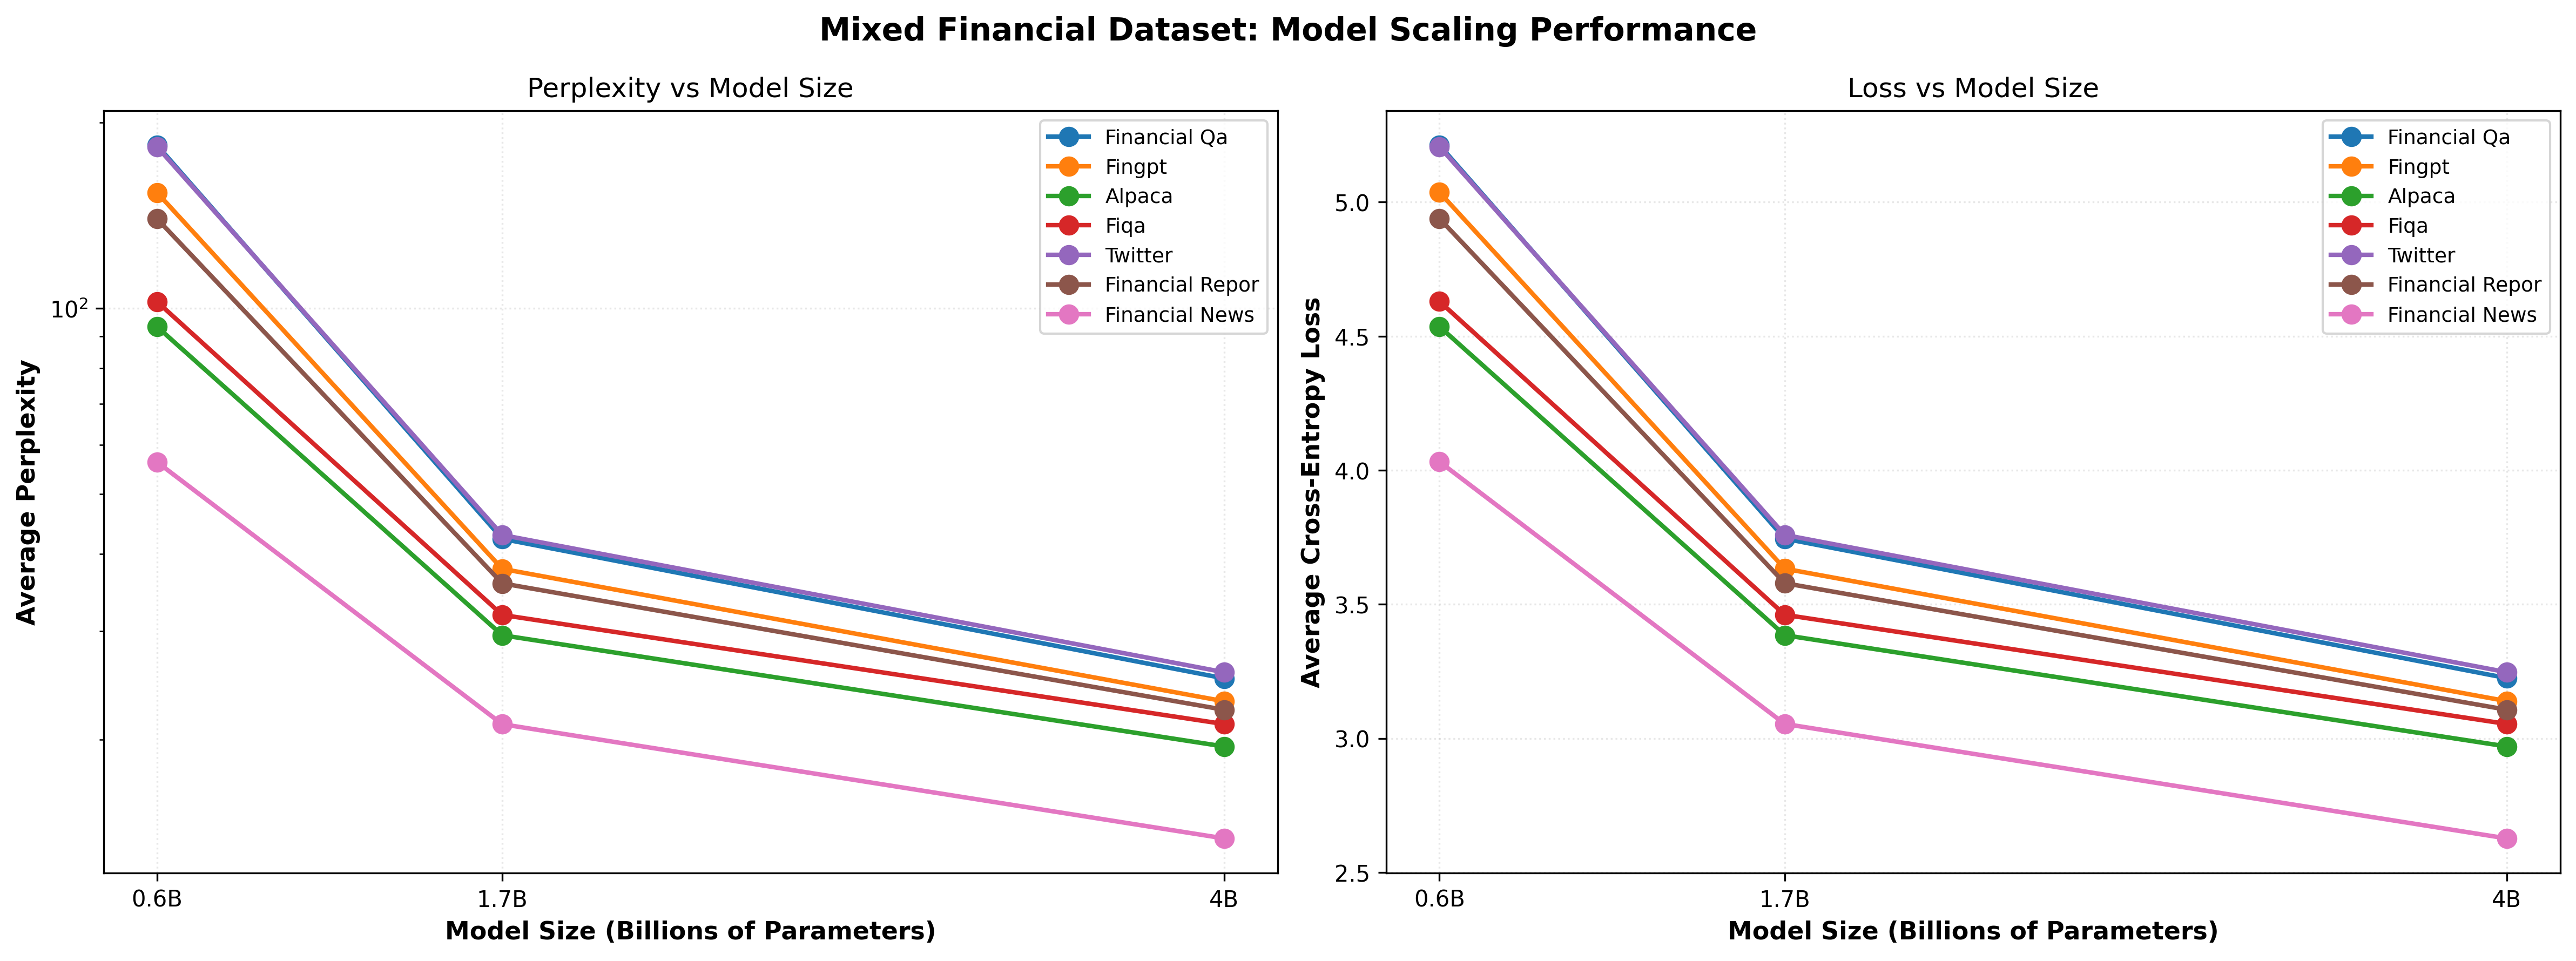
\includegraphics[width=0.9\textwidth]{figures/scaling_mixed_financial.png}
\caption[Mixed Financial Dataset: Scaling Behavior]{Mixed Financial Dataset: Model scaling behavior across 0.6B, 1.7B, and 4B parameters. Left panel shows perplexity (log scale) decreasing consistently with model size. Right panel shows cross-entropy loss following expected scaling pattern. Both metrics demonstrate normal scaling with 22.6\% total improvement from 0.6B to 4B.}
\label{fig:scaling_mixed_financial}
\end{figure}

% Mixed Financial Dataset: Evaluation Results
% Training: Mixed Financial (7 datasets mixed, 322M tokens)
% All models trained with LR=2e-5

\begin{table}[h]
\centering
\caption{Mixed Financial Dataset: Evaluation Across Multiple Datasets}
\label{tab:mixed_financial_results}
\begin{tabular}{l|ccc|ccc}
\hline
\textbf{Eval Dataset} & \multicolumn{3}{c|}{\textbf{Cross-Entropy Loss}} & \multicolumn{3}{c}{\textbf{Perplexity}} \\
\cline{2-4} \cline{5-7}
  & \textbf{0.6B} & \textbf{1.7B} & \textbf{4B} & \textbf{0.6B} & \textbf{1.7B} & \textbf{4B} \\
\hline
Alpaca & 4.54 & 3.38 & \textbf{2.97} & 93.35 & \textbf{29.53} & \textbf{19.50} \\
Financial News & 4.03 & 3.05 & \textbf{2.63} & 56.35 & \textbf{21.19} & \textbf{13.84} \\
Financial Qa & 5.21 & 3.75 & \textbf{3.23} & 183.7 & \textbf{42.30} & \textbf{25.14} \\
Financial Repor & 4.94 & 3.58 & \textbf{3.11} & 139.6 & \textbf{35.83} & \textbf{22.36} \\
Fingpt & 5.04 & 3.63 & \textbf{3.14} & 153.9 & \textbf{37.82} & \textbf{23.08} \\
Fiqa & 4.63 & 3.46 & \textbf{3.05} & 102.5 & \textbf{31.85} & \textbf{21.20} \\
Twitter & 5.21 & 3.76 & \textbf{3.25} & 182.6 & \textbf{42.91} & \textbf{25.72} \\
\hline
\end{tabular}
\end{table}



\subsection{Mixed Wiki+Financial}

Adding WikiText to the 7-dataset financial mixture (8 total datasets, 343M tokens) provides marginal benefits for general-domain performance but slightly degrades financial performance.

Performance scales across model sizes: 0.6B reached 75.00 ppl mean (across all eight evaluations including WikiText); 1.7B, 38.90; 4B, 26.69 (\Cref{tab:mixed_wiki_financial_results}). The 4B model's 26.69 ppl represents a 24\% increase over pure financial (21.55 ppl).

On the WikiText test set, the mixture achieves 27.72 ppl (4B). However, mean financial perplexity increases from 21.55 (pure financial; 4B) to \~26.55 (Wiki+Financial; 4B, financial-only mean), a \~23\% degradation. This trade-off is evident in \Cref{tab:mixed_wiki_financial_results}.

The mixture allocates approximately 28\% of tokens to WikiText (28.8M of 100M after 50cap normalization). For applications requiring both general and financial capabilities, this may be acceptable. But for finance-focused deployments, the performance loss on financial tasks outweighs general-domain gains.

We observe that variance is higher: 62\% (4B model) versus 55\% for pure financial, indicating increased spread across evaluation sets. The mixture struggles to balance the two domains, performing moderately on both rather than improving on either.

We believe that we should use Wiki+Financial mixture only when explicit general-domain performance is required and enough compute budget is ensured. For specialized financial applications with limited compute budget, pure financial mixture is superior.

\begin{figure}[htbp]
\centering
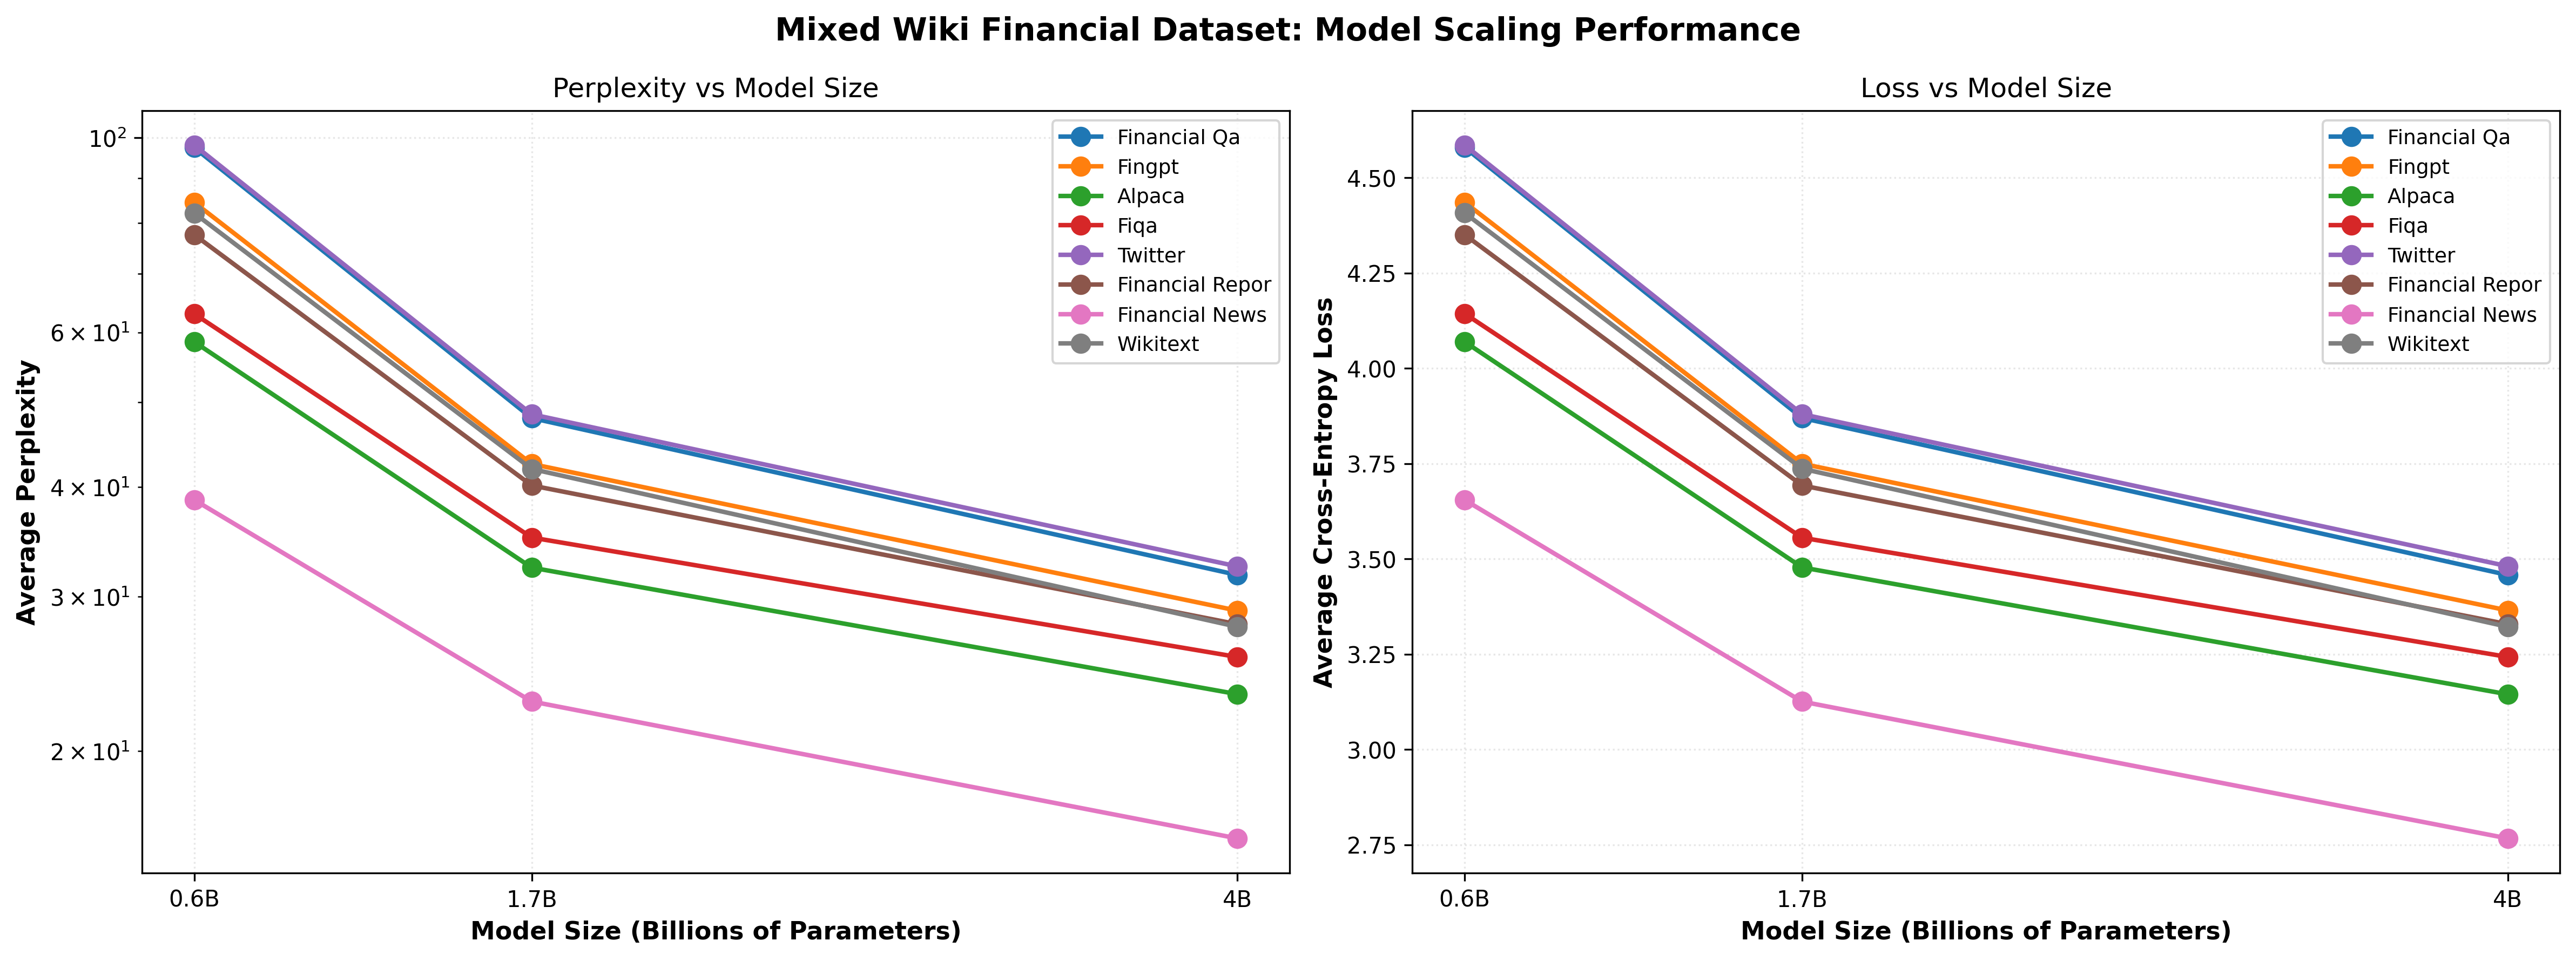
\includegraphics[width=0.9\textwidth]{figures/scaling_mixed_wiki_financial.png}
\caption[Mixed Wiki+Financial Dataset: Scaling Behavior]{Mixed Wiki+Financial Dataset: Scaling behavior shows normal pattern but with higher perplexity than pure financial mixture. The 15.1\% total improvement (0.6B to 4B) is smaller than pure financial (22.6\%), suggesting domain mixture creates competing optimization pressures that limit scaling benefits.}
\label{fig:scaling_mixed_wiki_financial}
\end{figure}

% Mixed Wiki+Financial Dataset: Evaluation Results
% Training: Mixed Wiki+Financial (WikiText + 7 financial datasets, ~400M tokens)
% All models trained with LR=2e-5

\begin{table}[h]
\centering
\caption{Mixed Wiki+Financial Dataset: Evaluation Across Multiple Datasets}
\label{tab:mixed_wiki_financial_results}
\resizebox{\textwidth}{!}{
\begin{tabular}{l|ccc|ccc}
\toprule
\multirow{2}{*}{\textbf{Eval Dataset}} &
\multicolumn{3}{c|}{\textbf{Cross-Entropy Loss}} &
\multicolumn{3}{c}{\textbf{Perplexity}} \\
\cmidrule(lr){2-4} \cmidrule(lr){5-7}
& \textbf{0.6B} & \textbf{1.7B} & \textbf{4B} & \textbf{0.6B} & \textbf{1.7B} & \textbf{4B} \\
\midrule
Alpaca & 4.07 & 3.48 & 3.15 & 58.56 & 32.38 & 23.23 \\
Financial News & 3.65 & 3.13 & 2.77 & 38.68 & 22.79 & 15.91 \\
Financial Qa & 4.58 & 3.87 & 3.46 & 97.49 & 47.94 & 31.76 \\
Financial Repor & 4.35 & 3.69 & 3.33 & 77.57 & 40.17 & 27.91 \\
Fingpt & 4.44 & 3.75 & 3.37 & 84.43 & 42.50 & 28.92 \\
Fiqa & 4.14 & 3.56 & 3.24 & 63.03 & 35.04 & 25.61 \\
Twitter & 4.59 & 3.88 & 3.48 & 98.13 & 48.42 & 32.48 \\
Wikitext & 4.41 & 3.74 & 3.32 & 82.10 & 41.95 & 27.72 \\
\bottomrule
\end{tabular}
}
\end{table}



\subsection{Pure WikiText Baseline}

Pretraining exclusively on WikiText-103 (124M tokens, ~0.8 epochs with 100M token budget) establishes a baseline for general-domain capabilities and tests cross-domain transfer to financial evaluation sets. The large dataset size results in undertraining (less than one full pass through the data).

The 0.6B model achieved 4.78 ppl (WikiText test set); 1.7B collapsed (infinite loss); 4B reached 31.54 ppl after LR adjustment to $1\times10^{-5}$. This experiment exhibited severe reverse scaling, this is resolved only through lowering the learning rates (see Section 4.4).

While 0.6B achieves excellent WikiText performance (4.78 ppl), financial evaluation reveals severe transfer failure. Mean financial perplexity (7 financial test sets): 0.6B: 10.38 ppl, 4B: 41.96 ppl (after LR fix). These values are 2-5$\times$ higher than mixed financial models, demonstrating that high-quality general corpora do not transfer effectively to specialized domains.

The 1.7B training collapse and 4B underperformance (before LR adjustment) suggest that WikiText's clean, structured data may be particularly sensitive to hyperparameter choices at larger scales. General corpora may require more careful tuning than noisy, diverse domain-specific mixtures.

\textbf{Key Takeaway}: Pure general-domain pretraining is insufficient for financial NLP and domain-specific pretraining is necessary. \Cref{tab:wikitext_lr_comparison} provides detailed metrics showing the dramatic difference between WikiText evaluation (where 0.6B excels at 4.78 ppl) and financial evaluations (where all models struggle with 40-60 ppl).

\begin{figure}[htbp]
\centering
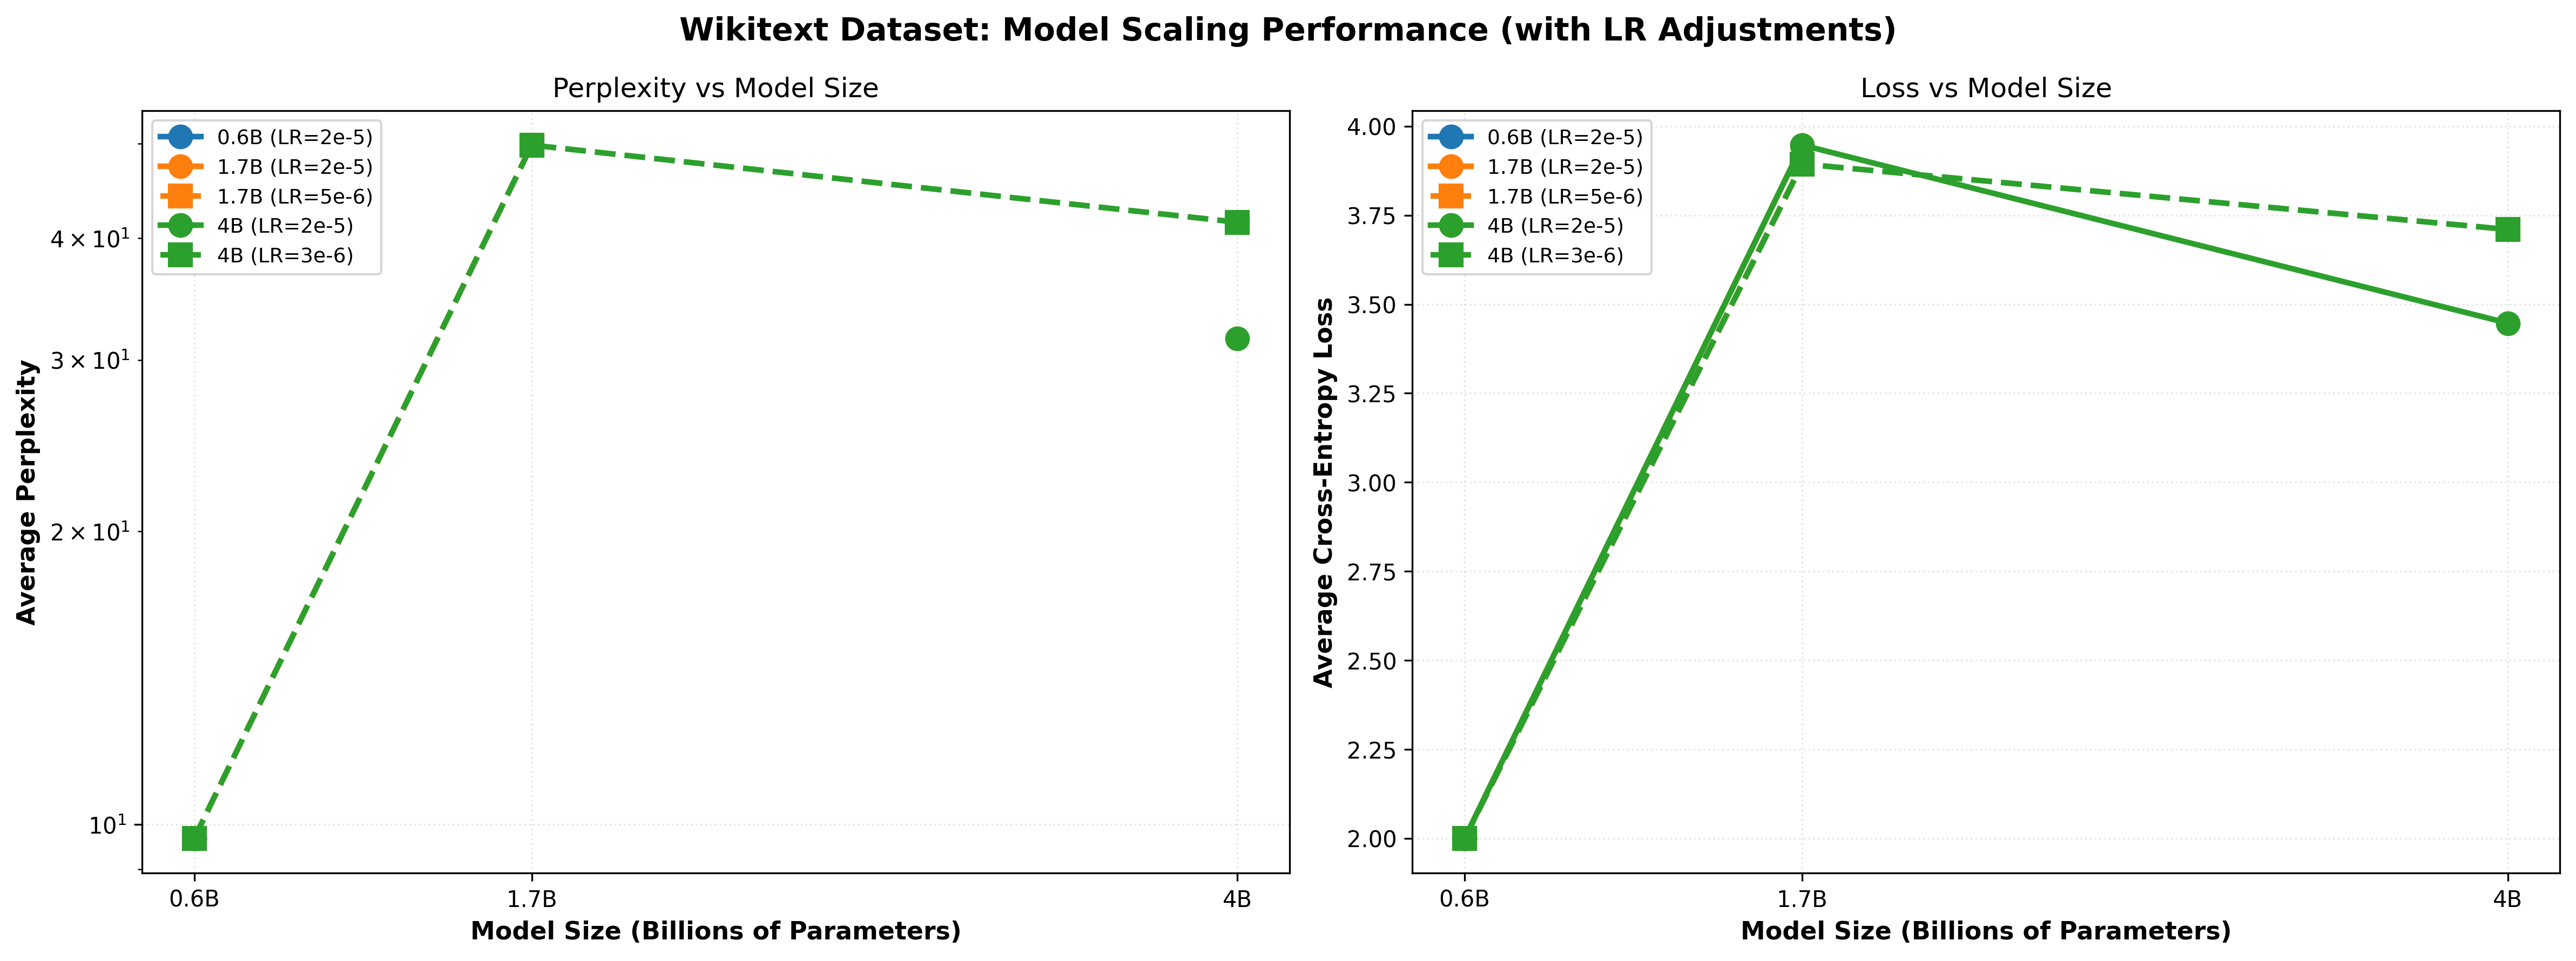
\includegraphics[width=0.9\textwidth]{figures/scaling_wikitext.png}
\caption[WikiText Dataset: Reverse Scaling]{WikiText Dataset: Severe reverse scaling phenomenon. The 1.7B model shows adjusted learning rate results (dashed line, squares) after fixing training collapse. The 4B model required 75\% LR reduction to stabilize. Clean, structured data amplifies learning rate sensitivity at larger scales.}
\label{fig:scaling_wikitext}
\end{figure}

% WikiText Dataset: Evaluation Results with LR Adjustments
% Training: WikiText (WikiText-103, 100M tokens)
% LR Adjustments: 1.7B (2e-5 → 5e-6), 4B (2e-5 → 3e-6)

\begin{table}[h]
\centering
\caption[WikiText: Learning Rate Comparison]{WikiText Dataset: Impact of Learning Rate Adjustments}
\label{tab:wikitext_lr_comparison}
\begin{tabular}{l|c|cc|cc|c|cc|cc}
\hline
\multirow{3}{*}{\textbf{Eval Dataset}} &
\multicolumn{5}{c|}{\textbf{Cross-Entropy Loss}} &
\multicolumn{5}{c}{\textbf{Perplexity}} \\
\cline{2-6} \cline{7-11}
& \textbf{0.6B} & \multicolumn{2}{c|}{\textbf{1.7B}} & \multicolumn{2}{c|}{\textbf{4B}} &
 \textbf{0.6B} & \multicolumn{2}{c|}{\textbf{1.7B}} & \multicolumn{2}{c}{\textbf{4B}} \\
\cline{3-4} \cline{5-6} \cline{8-9} \cline{10-11}
& \textbf{2e-5} & \textbf{2e-5} & \textbf{5e-6} & \textbf{2e-5} & \textbf{3e-6} &
 \textbf{2e-5} & \textbf{2e-5} & \textbf{5e-6} & \textbf{2e-5} & \textbf{3e-6} \\
\hline
 Alpaca & 2.22 & \textbf{3.24} & 3.79 & \textbf{3.48} & 3.64 & 9.23 & \textbf{25.51} & 44.22 & \textbf{32.38} & 38.06 \\
Financial News & 2.62 & \textbf{2.93} & 3.52 & 3.37 & \textbf{3.27} & 13.70 & \textbf{18.78} & 33.66 & \textbf{29.19} & \textbf{26.44} \\
 Financial QA & 3.40 & 10.67 & \textbf{4.07} & \textbf{3.37} & 3.87 & 29.90 & $\infty$ & \textbf{58.33} & \textbf{29.08} & 47.98 \\
 SEC Reports & 1.39 & \textbf{3.27} & 3.91 & \textbf{3.44} & 3.75 & 3.99 & \textbf{26.46} & 49.83 & \textbf{31.23} & 42.41 \\
 FinGPT & 1.30 & \textbf{2.11} & 4.07 & \textbf{3.57} & 3.88 & 3.67 & \textbf{8.27} & 58.55 & \textbf{35.50} & 48.30 \\
 FiQA & 2.07 & \textbf{3.14} & 3.85 & \textbf{3.53} & 3.74 & 7.89 & \textbf{23.15} & 46.81 & \textbf{34.03} & 42.04 \\
Twitter & 1.45 & \textbf{2.78} & 4.08 & \textbf{3.52} & 3.88 & 4.26 & \textbf{16.06} & 58.98 & \textbf{33.71} & 48.48 \\
\rowcolor{gray!20} \textbf{Wikitext (train)} & 1.56 & \textbf{3.42} & 3.88 & \textbf{3.30} & 3.65 & 4.78 & \textbf{30.63} & 48.44 & \textbf{27.19} & 38.60 \\
\rowcolor{blue!10} \textbf{Average} & \textbf{2.00} & \textbf{3.95} & \textbf{3.89} & \textbf{3.45} & \textbf{3.71} & \textbf{9.68} & \textbf{$\infty$} & \textbf{49.85} & \textbf{31.54} & \textbf{41.54}  \\
\hline
\end{tabular}
\end{table}


\begin{figure}[htbp]
\centering
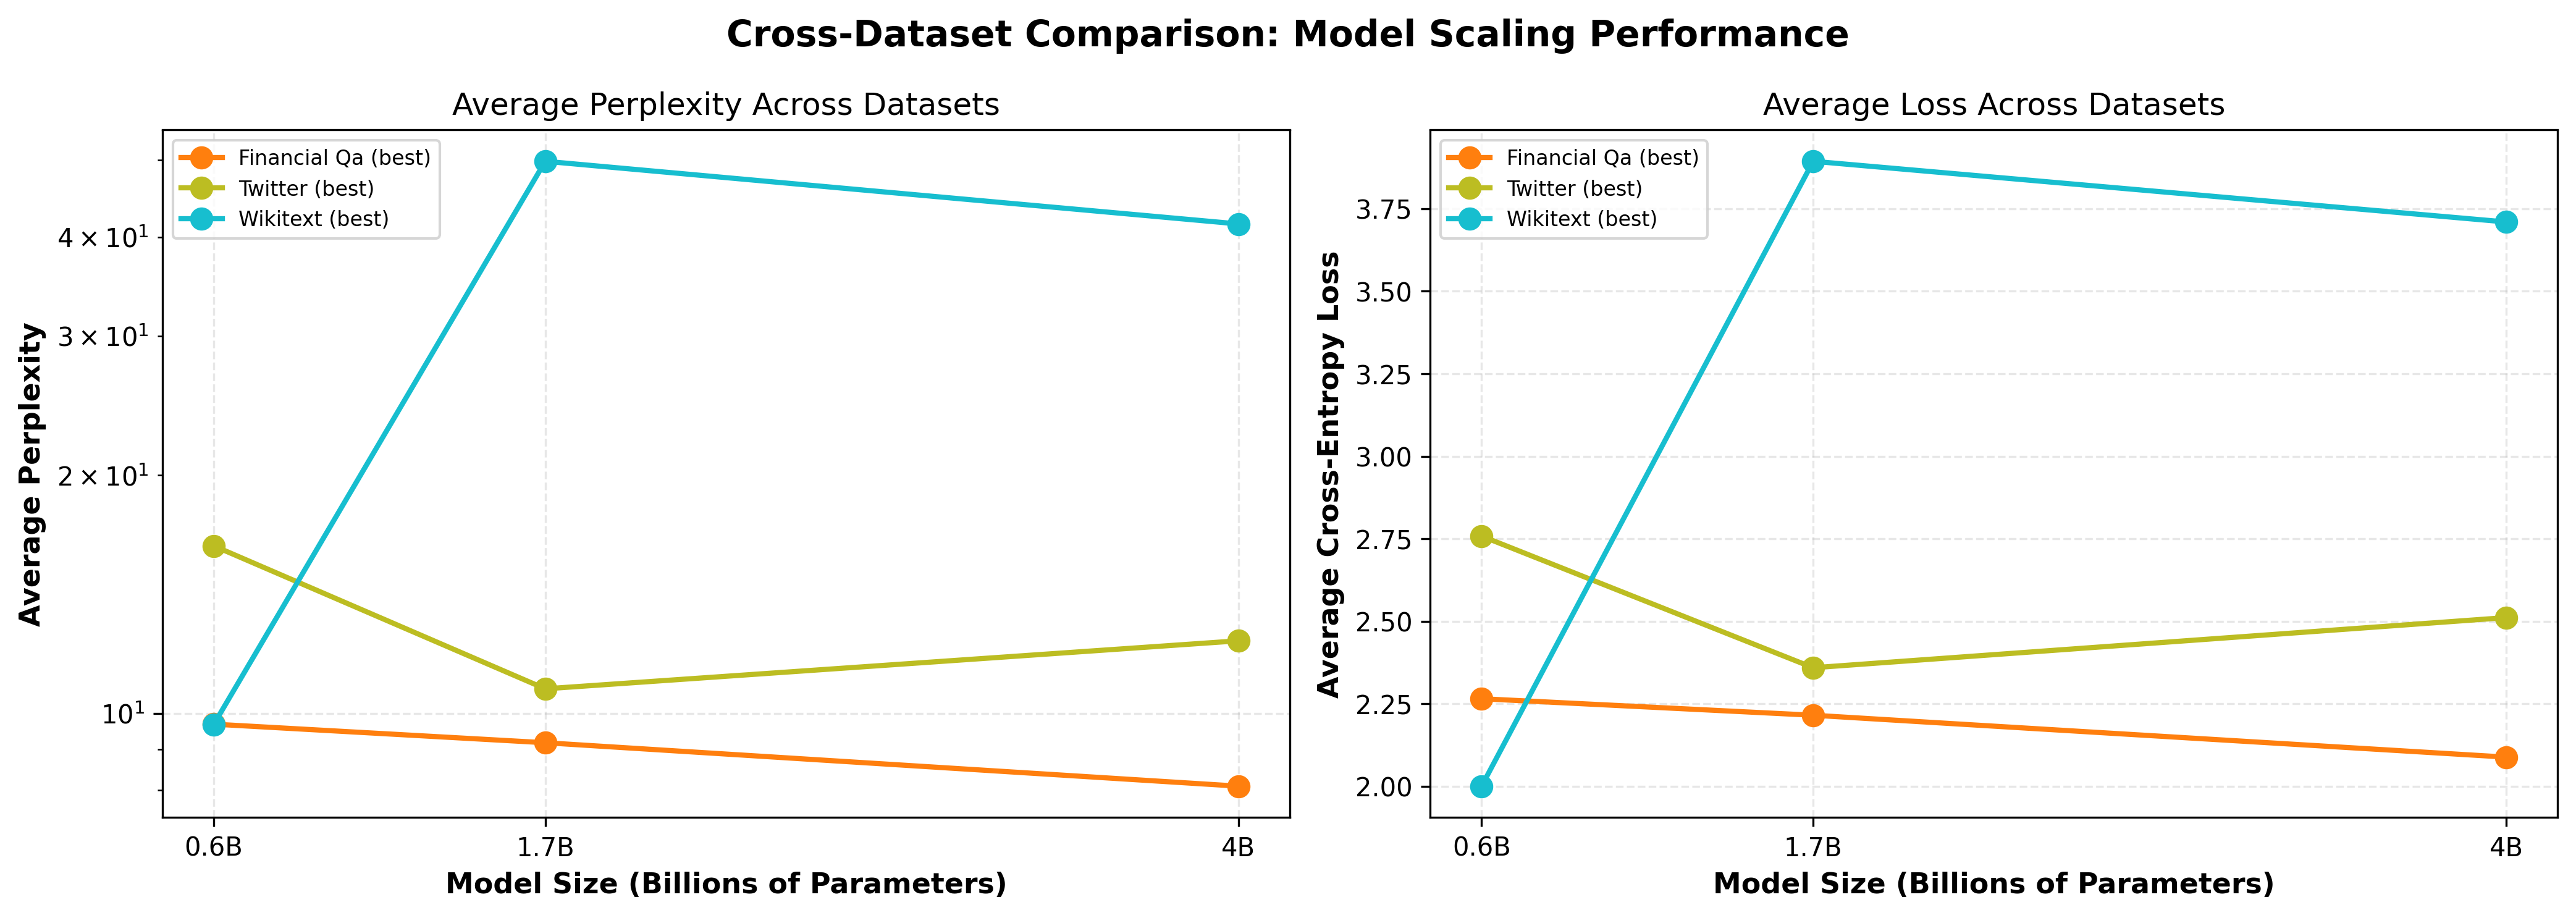
\includegraphics[width=0.9\textwidth]{figures/scaling_comparison_all.png}
\caption[Comparison of Mixture Strategies]{Comparison of all three mixture strategies across model sizes. Mixed Financial (blue) consistently outperforms Mixed Wiki+Financial (orange) and WikiText (green) on financial evaluation metrics. The divergence increases with model size, demonstrating that in-domain diversity scales better than general-domain quality.}
\label{fig:scaling_comparison_all}
\end{figure}

\section{Individual Dataset Analysis: Component Effects}

To understand which datasets contribute most to mixture performance and when standalone pretraining is viable, we trained models on each of the 7 financial datasets individually. Results reveal a clear relationship between dataset size and pretraining viability.

\subsection{Large Datasets}

News Articles (194M tokens) trained for only 0.5 epochs (severe undertraining). Performance on the News test set improves cleanly with scale (0.6B: 52.25 ppl; 1.7B: 22.91; 4B: 17.47), i.e., 56\% from 0.6B→1.7B and a further 24\% from 1.7B→4B. However, average perplexity across all test sets (32.82 ppl) is 2–5$\times$ worse than medium datasets, suggesting undertraining limits generalization. Transfer is strongest to SEC (33.46 ppl), Alpaca (29.75 ppl), and FiQA (31.69 ppl), and weaker to FinGPT (38.03 ppl), Twitter (38.98 ppl) and Financial QA (38.90 ppl).

\textbf{Summary}: News (194M, 0.5 epochs, 32.82 ppl) demonstrates that large dataset size alone does not guarantee quality, possibly because undertraining ($<$1 epoch) provides insufficient exposure to data despite large vocabulary coverage. \Cref{fig:scaling_news_articles} demonstrates clean scaling curves with no reverse scaling, but undertraining prevents News from achieving competitive average performance.

\begin{figure}[htbp]
\centering
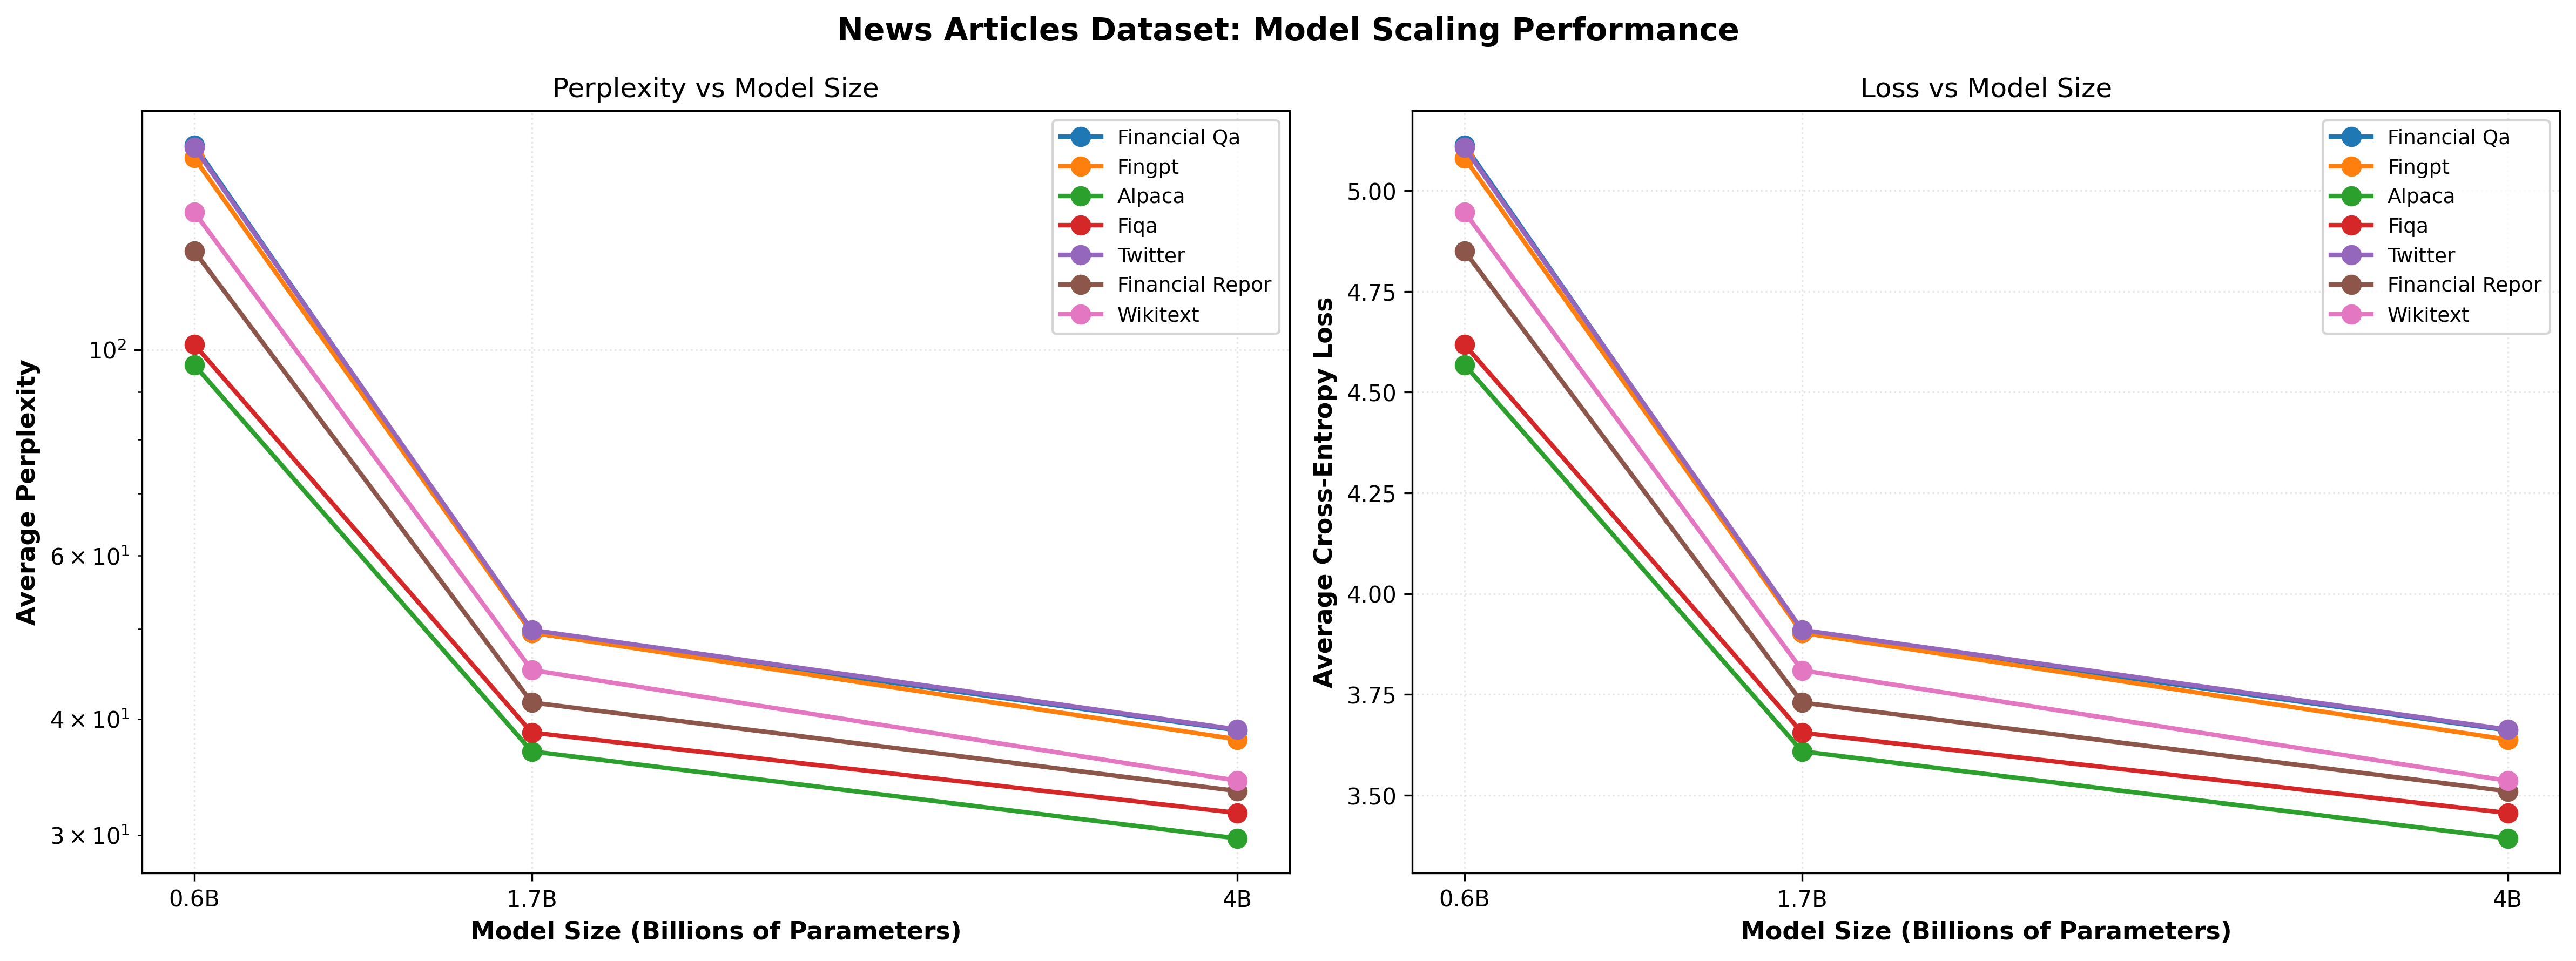
\includegraphics[width=0.9\textwidth]{figures/scaling_news_articles.png}
\caption[Financial News Dataset: Scaling Behavior]{Financial News Articles Dataset: Normal scaling with 66.6\% total improvement (0.6B to 4B), but severe undertraining (0.5 epochs) limits generalization. Average perplexity (32.82 ppl) is 2–5$\times$ worse than medium datasets, demonstrating that dataset size alone does not guarantee quality—optimal epoch count matters more.}
\label{fig:scaling_news_articles}
\end{figure}

\begin{figure}[htbp]
\centering
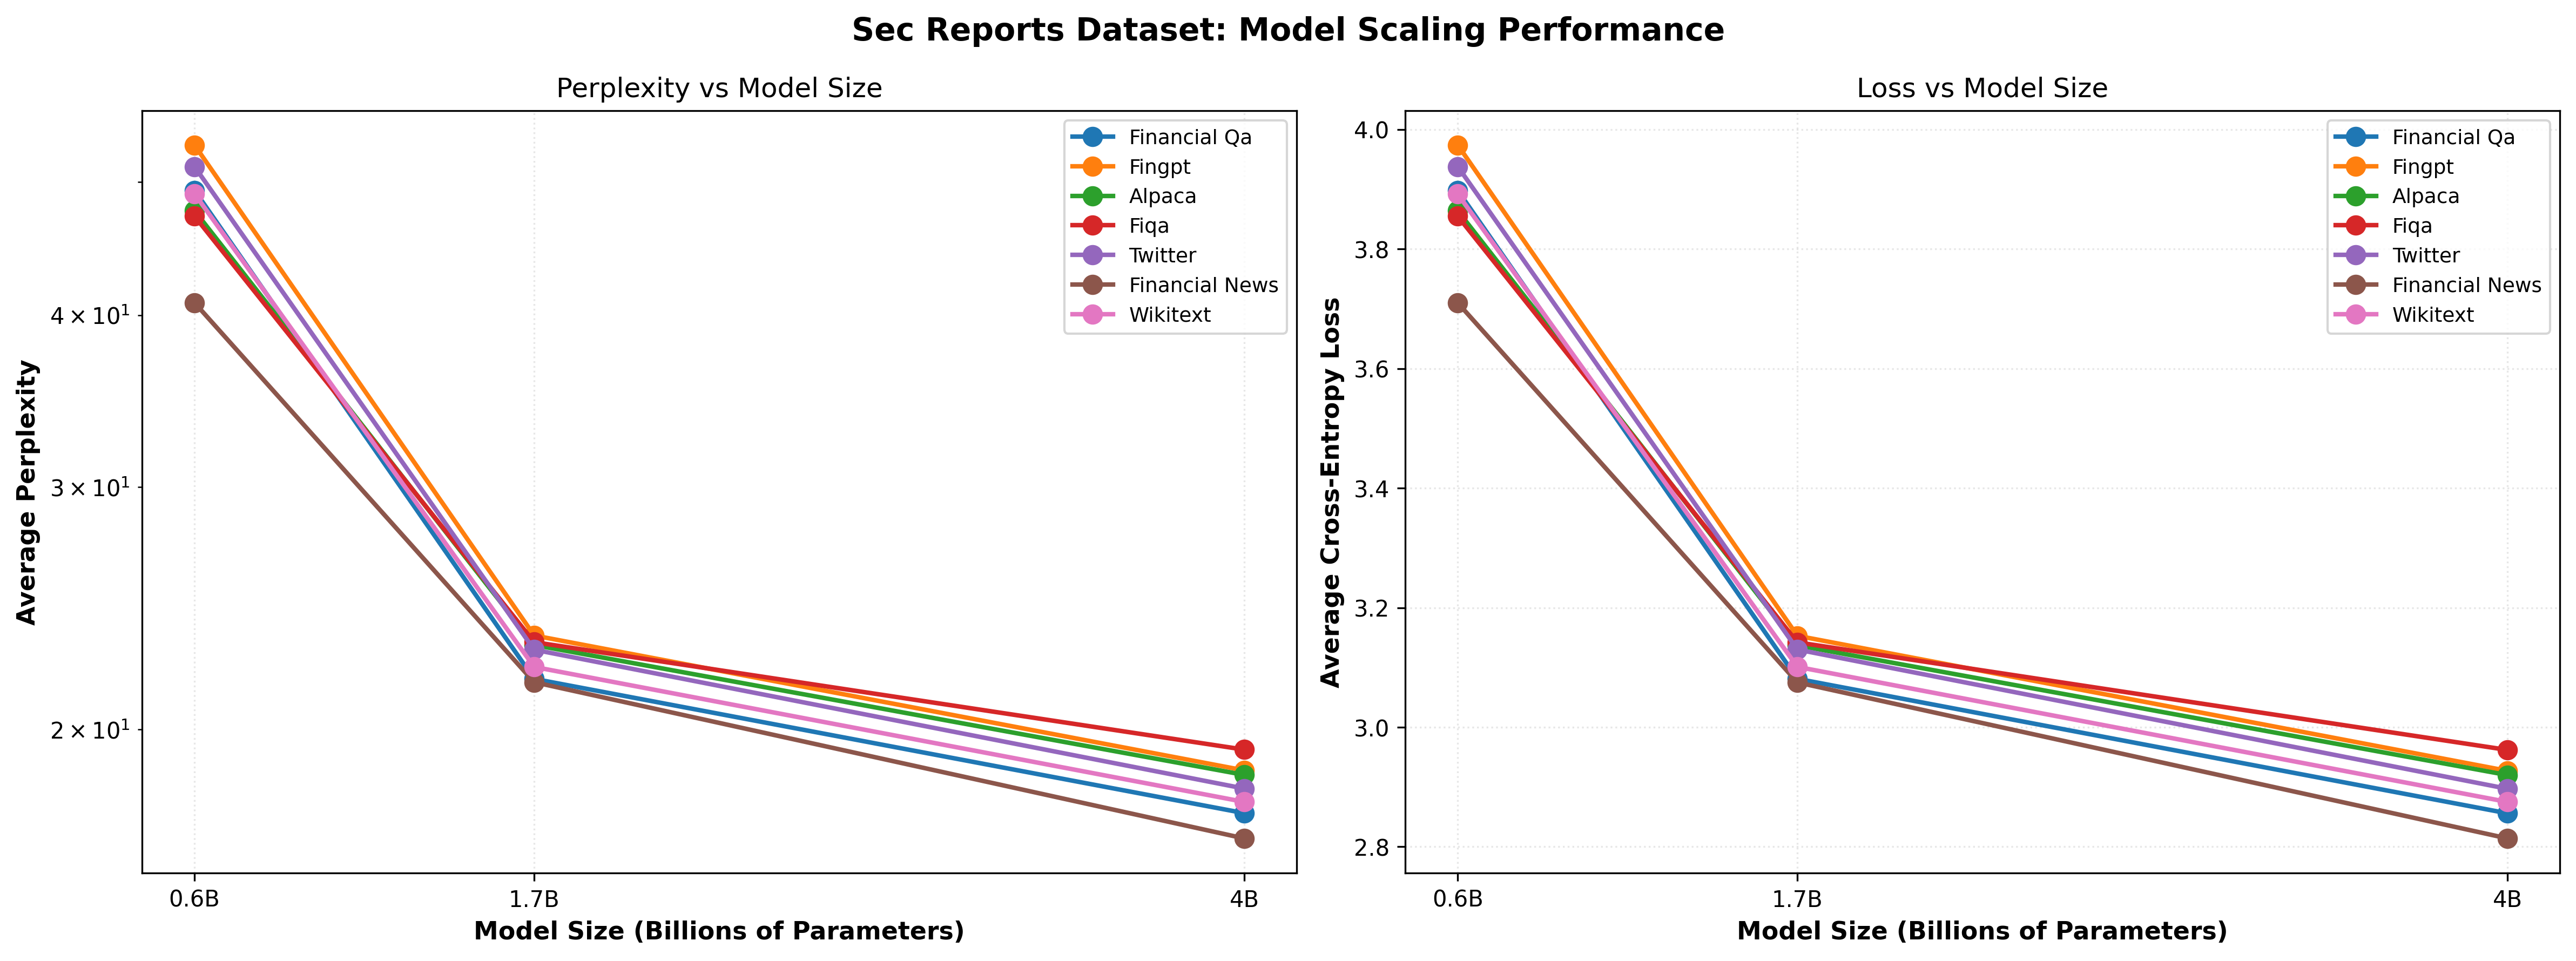
\includegraphics[width=0.9\textwidth]{figures/scaling_sec_reports.png}
\caption[SEC Reports Dataset: Scaling Behavior]{SEC Reports Dataset: Excellent normal scaling with 61.3\% total improvement. The 8.1M token corpus achieves optimal training dynamics (~12 epochs), resulting in strong average performance (17.80 ppl) that outperforms much larger datasets. Exemplifies medium-sized dataset superiority.}
\label{fig:scaling_sec_reports}
\end{figure}

% Financial News Dataset: Evaluation Results
% Training: Financial News (Financial news articles, 194.47M tokens)
% All models trained with LR=2e-5

\begin{table}[htbp]
\centering
\caption[Financial News: Evaluation Results]{Financial News Dataset: Evaluation Across Multiple Datasets}
\label{tab:news_articles_results}
\begin{tabular}{l|ccc|ccc}
\hline
\textbf{Eval Dataset} & \multicolumn{3}{c|}{\textbf{Cross-Entropy Loss}} & \multicolumn{3}{c}{\textbf{Perplexity}} \\
\cline{2-4} \cline{5-7}
  & \textbf{0.6B} & \textbf{1.7B} & \textbf{4B} & \textbf{0.6B} & \textbf{1.7B} & \textbf{4B} \\
\hline
Alpaca & 4.57 & 3.61 & \textbf{3.39} & 96.31 & \textbf{36.92} & \textbf{29.75} \\
\textbf{Financial News} & \textbf{3.96} & \textbf{3.13} & \textbf{2.86} & \textbf{52.25} & \textbf{22.91} & \textbf{17.47} \\
Financial QA & 5.11 & 3.90 & \textbf{3.66} & 166.1 & \textbf{49.53} & \textbf{38.90} \\
SEC Reports & 4.85 & 3.73 & \textbf{3.51} & 127.7 & \textbf{41.68} & \textbf{33.46} \\
FinGPT & 5.08 & 3.90 & \textbf{3.64} & 160.9 & \textbf{49.56} & \textbf{38.03} \\
FiQA & 4.62 & 3.65 & \textbf{3.46} & 101.3 & \textbf{38.68} & \textbf{31.69} \\
Twitter & 5.11 & 3.91 & \textbf{3.66} & 165.2 & \textbf{49.88} & \textbf{38.98} \\
Wikitext & 4.95 & 3.81 & \textbf{3.54} & 140.7 & \textbf{45.17} & \textbf{34.33} \\
\hline
\textbf{Average} & \textbf{4.78} & \textbf{3.71} & \textbf{3.47} & \textbf{126.3} & \textbf{41.79} & \textbf{32.82} \\
\hline
\end{tabular}
\end{table}


% SEC Reports Dataset: Evaluation Results
% Training: SEC Reports (SEC 10-K/10-Q filings, 80M tokens)
% All models trained with LR=2e-5

\begin{table}[h]
\centering
\caption[SEC Reports: Evaluation Results]{SEC Reports Dataset: Evaluation Across Multiple Datasets}
\label{tab:sec_reports_results}
\begin{tabular}{l|ccc|ccc}
\hline
\textbf{Eval Dataset} & \multicolumn{3}{c|}{\textbf{Cross-Entropy Loss}} & \multicolumn{3}{c}{\textbf{Perplexity}} \\
\cline{2-4} \cline{5-7}
  & \textbf{0.6B} & \textbf{1.7B} & \textbf{4B} & \textbf{0.6B} & \textbf{1.7B} & \textbf{4B} \\
Alpaca & 3.86 & 3.14 & \textbf{2.92} & 47.65 & \textbf{23.04} & \textbf{18.54} \\
Financial News & 3.71 & 3.08 & \textbf{2.81} & 40.85 & \textbf{21.65} & \textbf{16.67} \\
Financial Qa & 3.90 & 3.08 & \textbf{2.86} & 49.30 & \textbf{21.77} & \textbf{17.39} \\
Fingpt & 3.97 & 3.15 & \textbf{2.93} & 53.18 & \textbf{23.41} & \textbf{18.68} \\
Fiqa & 3.85 & 3.14 & \textbf{2.96} & 47.22 & \textbf{23.15} & \textbf{19.34} \\
Twitter & 3.94 & 3.13 & \textbf{2.90} & 51.30 & \textbf{22.86} & \textbf{18.12} \\
Wikitext & 3.89 & 3.10 & \textbf{2.88} & 49.02 & \textbf{22.21} & \textbf{17.72} \\
\hline
\end{tabular}
\end{table}



\subsection{Medium Datasets}

Four datasets range from 3.6–8.5M tokens: SEC Reports (8.1M), Finance Alpaca (8.5M), FinGPT Sentiment (4.1M), FiQA (3.6M). These achieve optimal epoch counts (12–28 epochs) and demonstrate the sweet spot for performance.

SEC Reports (8.1M tokens) trained for ~12 epochs. On the SEC test set, scaling behaves as expected (0.6B: 41.12 ppl; 1.7B: 19.36; 4B: 15.91). Average perplexity across all test sets (17.80 ppl) places SEC among one of the best-performing individual datasets, demonstrating that medium-sized datasets with optimal epoch counts outperform large undertrained datasets. Transfer is strong to other datasets, including News (16.67 ppl, similar long‑form structure), FinGPT (18.68), Alpaca (18.54), FiQA (19.34), Twitter (18.12), and Financial QA (17.39). The 4B SEC model shows 19\% relative spread across evaluations, demonstrating excellent consistency. Both News and SEC models transfer well to each other, suggesting that document length and narrative structure drive transferability.

FinGPT Sentiment (4.1M tokens) trained for 24 epochs. On its own test set, performance scales strongly (0.6B: 32.78 ppl; 1.7B: 9.56; 4B: 5.67). Transfer to other datasets is also strong, such as Alpaca (8.27) and FiQA (8.16). The 4B model's relative spread is 37.07\%, reflecting task‑type specialization.

Finance Alpaca (8.5M tokens) trained for 12 epochs. On Alpaca, scaling is clear (0.6B: 63.73 ppl; 1.7B: 15.61; 4B: 8.22). Similar to above datasets, we see strong transfer to other evaluation datasets. The 4B model's variance (11.51\% spread) reflects its narrow task focus.

FiQA (3.6M tokens) trained for 28 epochs. On FiQA, scaling is strong (0.6B: 64.75 ppl; 1.7B: 12.99; 4B: 7.08). Transfer is also good on other datasets. The 4B model shows 18.97\% relative spread.

\textbf{Summary}: Medium datasets (3.6 to 8.5M tokens, 12-28 epochs) achieve optimal training dynamics. Training on these datasets transfer well to other datasets, both in-domain and out-of-domain \Cref{fig:scaling_sec_reports,fig:scaling_fingpt,fig:scaling_alpaca,fig:scaling_fiqa} and \Cref{tab:sec_reports_results,tab:fingpt_results,tab:alpaca_results,tab:fiqa_results} show performance of training on these medium-sized datasets.

\begin{figure}[htbp]
\centering
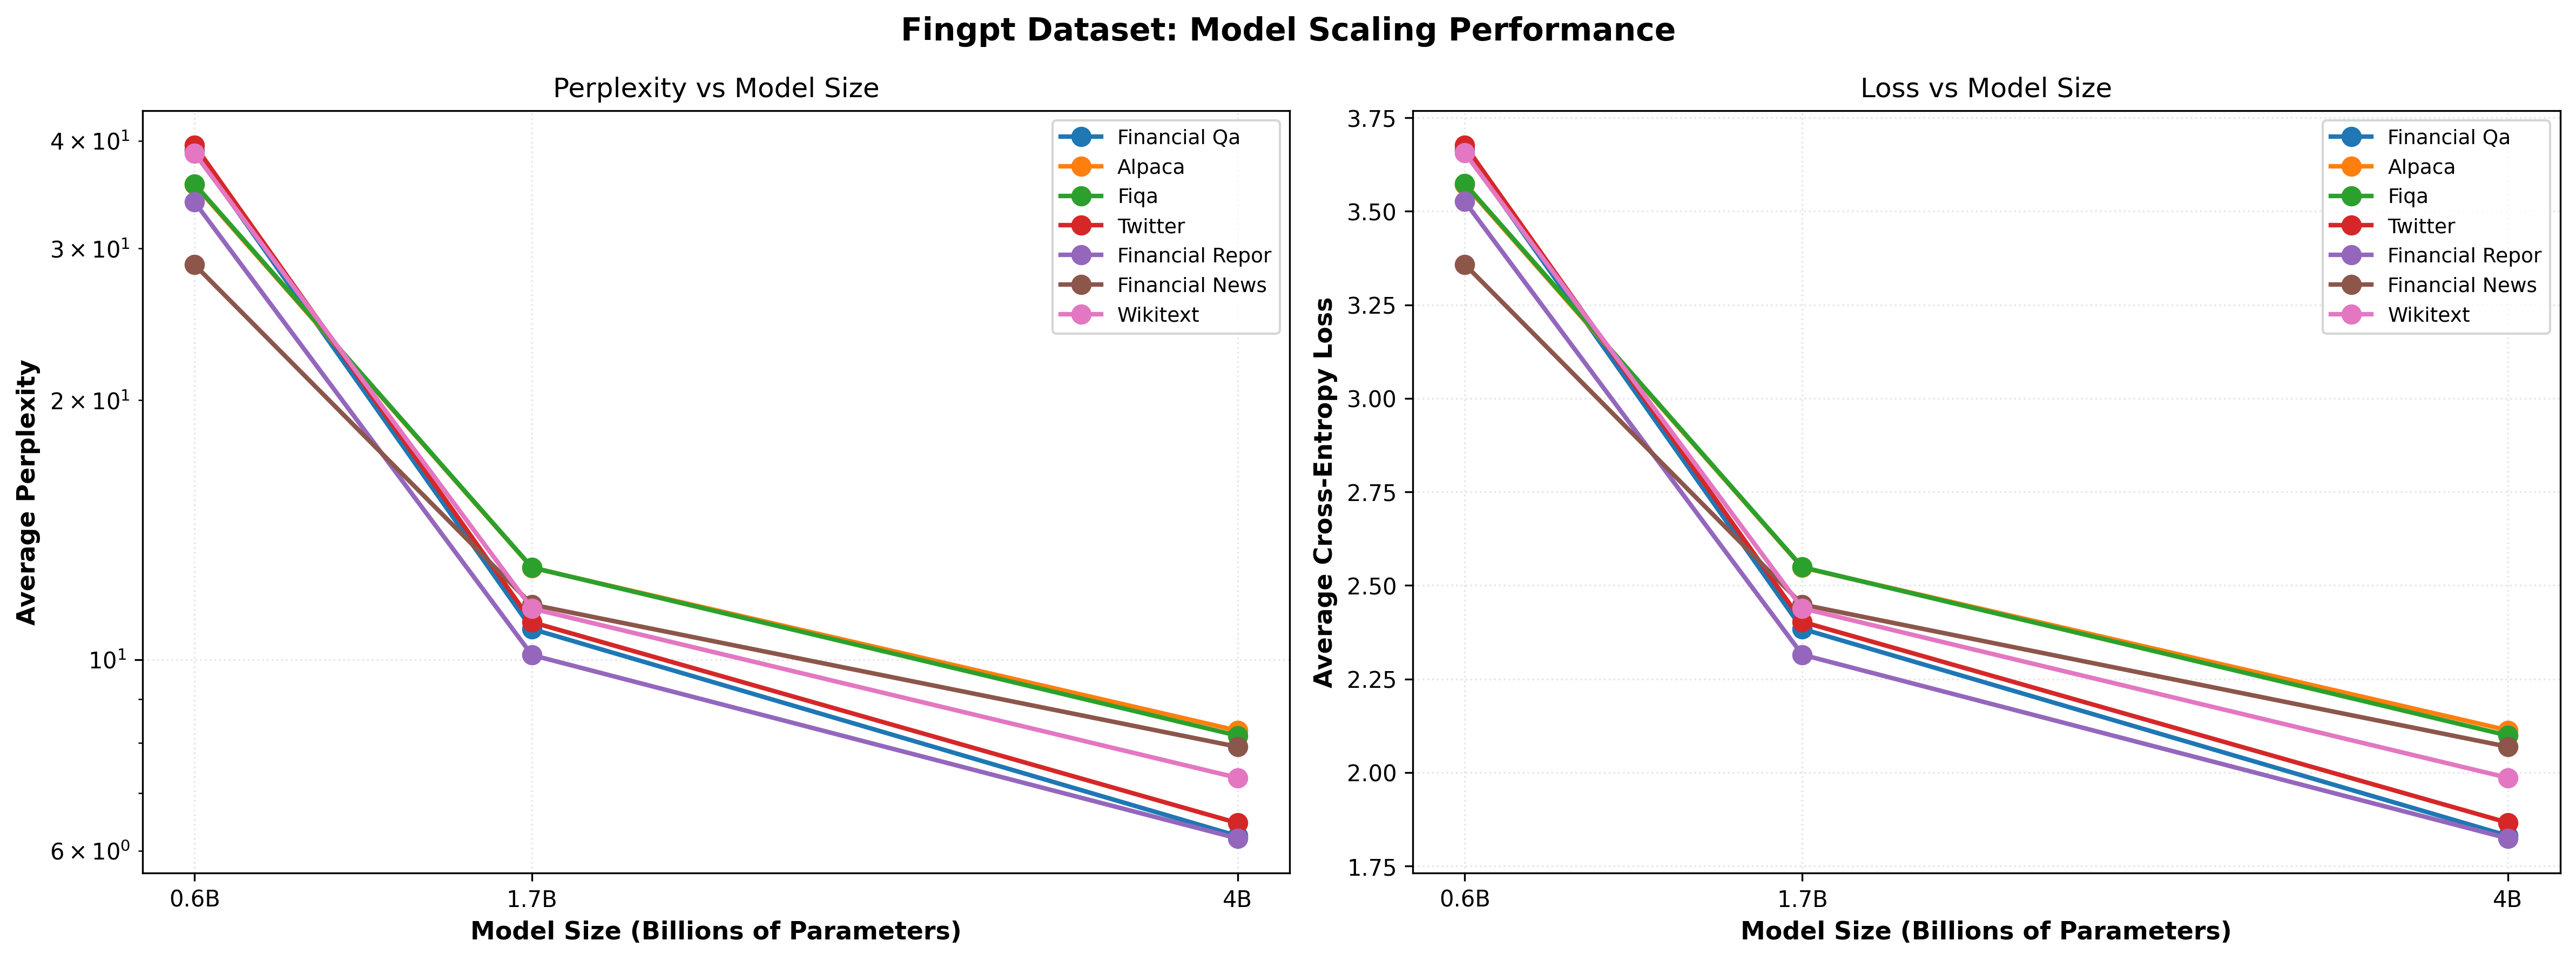
\includegraphics[width=0.9\textwidth]{figures/scaling_fingpt.png}
\caption[FinGPT Sentiment Dataset: Scaling Behavior]{FinGPT Sentiment Dataset: Normal scaling with 82.7\% improvement despite moderate overtraining (24 epochs). Instruction-following format benefits from increased model capacity, showing strong transfer to similar task types.}
\label{fig:scaling_fingpt}
\end{figure}

\begin{figure}[htbp]
\centering
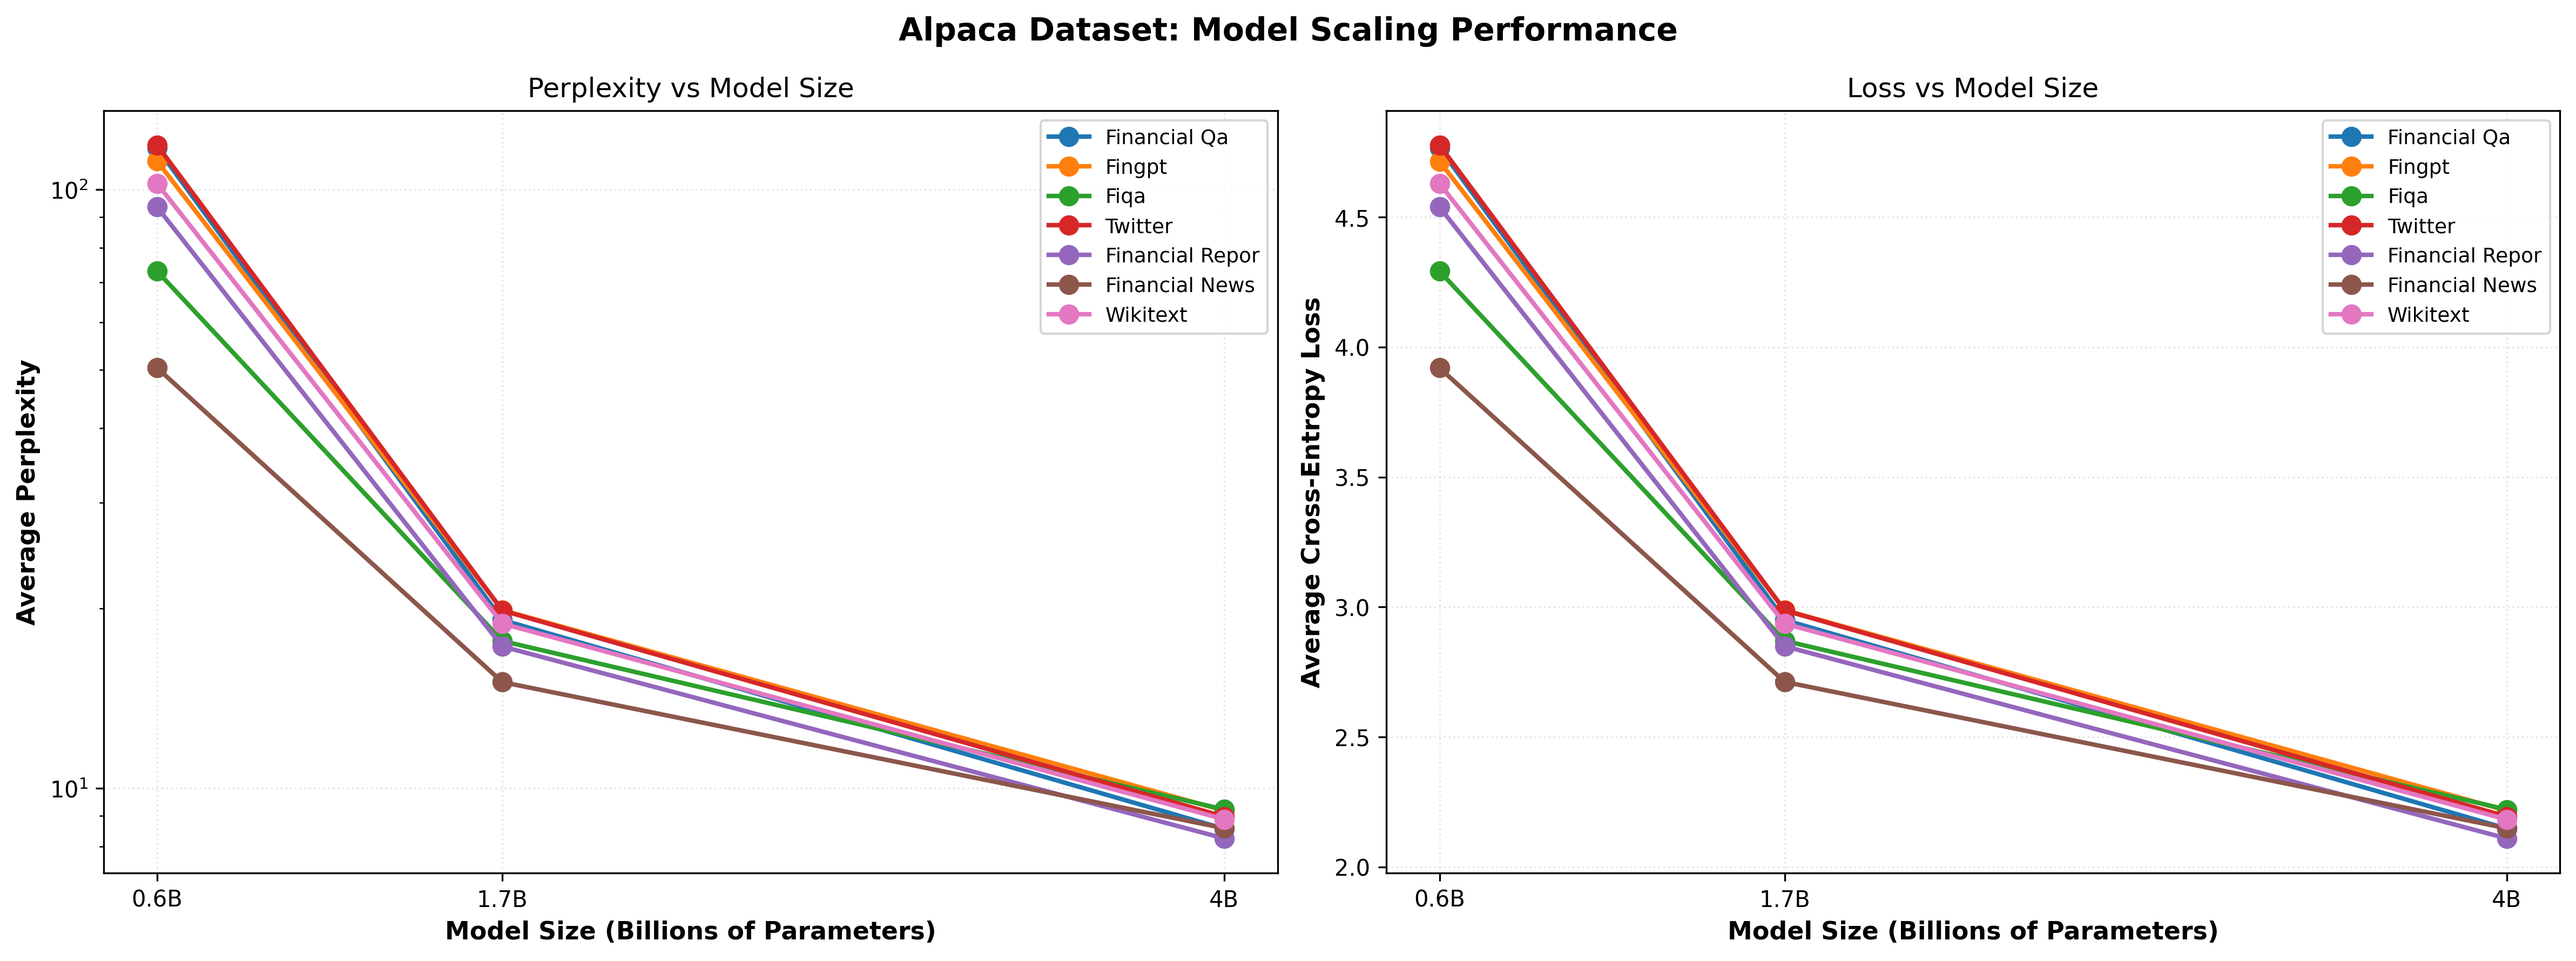
\includegraphics[width=0.9\textwidth]{figures/scaling_alpaca.png}
\caption[Finance Alpaca Dataset: Scaling Behavior]{Finance Alpaca Dataset: Consistent 87.1\% improvement across model sizes. Educational Q\&A format shows reliable scaling despite 12 epochs of training, but exhibits narrow task focus with 11.51\% cross-dataset variance.}
\label{fig:scaling_alpaca}
\end{figure}

\begin{figure}[htbp]
\centering
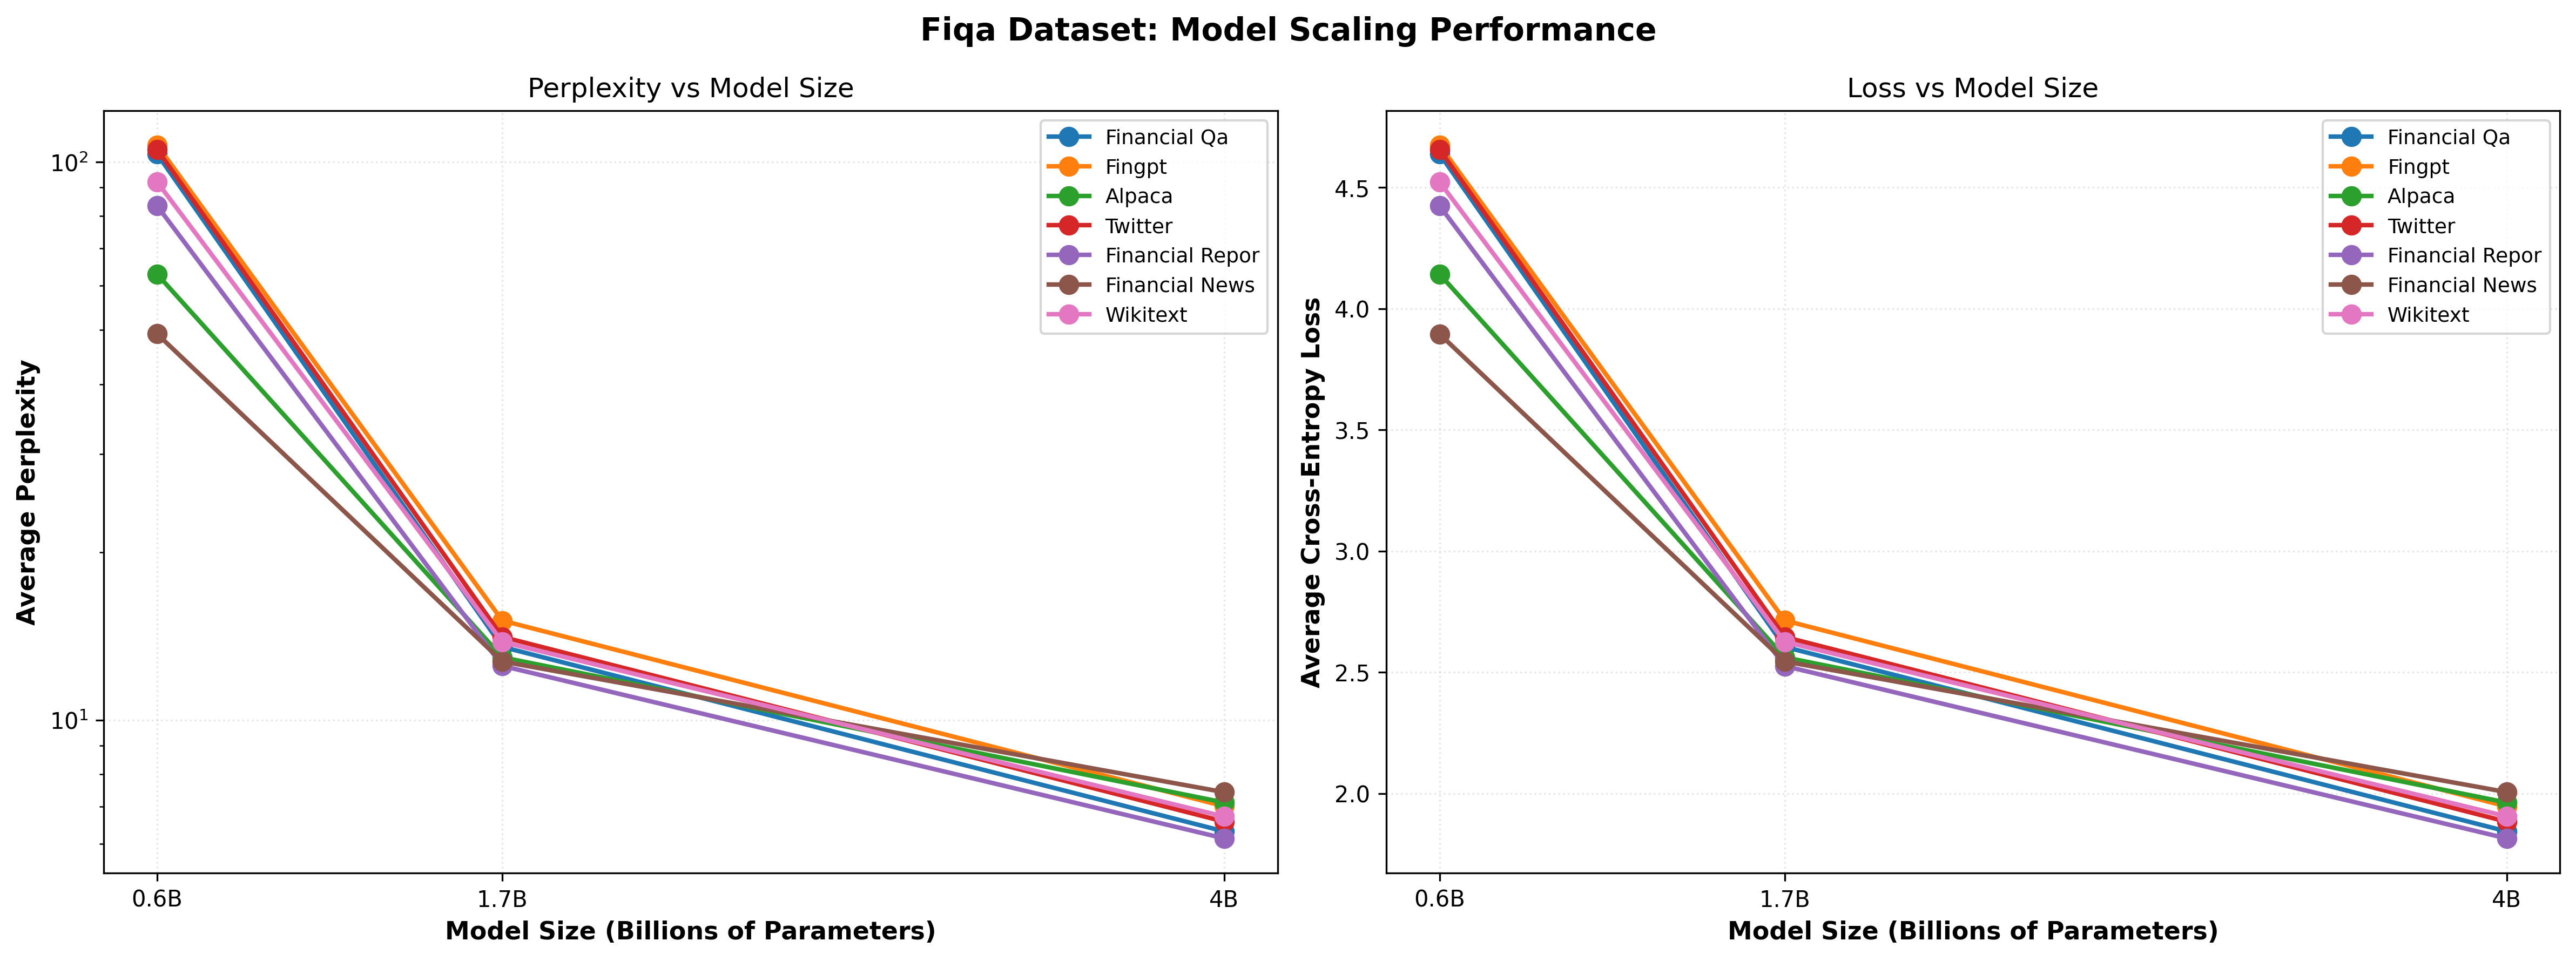
\includegraphics[width=0.9\textwidth]{figures/scaling_fiqa.png}
\caption[FiQA Dataset: Scaling Behavior]{FiQA Dataset: Strong normal scaling with 89.1\% total improvement. Despite small size (4M tokens), conversational Q\&A format produces stable training and excellent in-domain performance, though with high variance (18.97\%) on out-of-format tasks.}
\label{fig:scaling_fiqa}
\end{figure}

% FinGPT Sentiment Dataset: Evaluation Results
% Training: FinGPT Sentiment (FinGPT/fingpt-sentiment-train, 19M tokens)
% All models trained with LR=2e-5

\begin{table}[h]
\centering
\caption{FinGPT Sentiment Dataset: Evaluation Across Multiple Datasets}
\label{tab:fingpt_results}
\begin{tabular}{l|ccc|ccc}
\hline
\textbf{Eval Dataset} & \multicolumn{3}{c|}{\textbf{Cross-Entropy Loss}} & \multicolumn{3}{c}{\textbf{Perplexity}} \\n\cline{2-4} \cline{5-7}
  & \textbf{0.6B} & \textbf{1.7B} & \textbf{4B} & \textbf{0.6B} & \textbf{1.7B} & \textbf{4B} \\
Alpaca & 3.57 & 2.55 & \textbf{2.11} & 35.55 & \textbf{12.78} & \textbf{8.27} \
 Financial News & 3.36 & 2.45 & \textbf{2.07} & 28.72 & \textbf{11.58} & \textbf{7.92} \
 Financial Qa & 3.66 & 2.38 & \textbf{1.83} & 38.96 & \textbf{10.85} & \textbf{6.24} \
 Financial Repor & 3.53 & 2.31 & \textbf{1.82} & 33.97 & \textbf{10.12} & \textbf{6.20} \
 Fiqa & 3.57 & 2.55 & \textbf{2.10} & 35.64 & \textbf{12.79} & \textbf{8.16} \
 Twitter & 3.68 & 2.40 & \textbf{1.87} & 39.54 & \textbf{11.05} & \textbf{6.46} \
 Wikitext & 3.66 & 2.44 & \textbf{1.99} & 38.70 & \textbf{11.46} & \textbf{7.29} \
\hline
\end{tabular}
\end{table}



% Finance Alpaca Dataset: Evaluation Results
% Training: Finance Alpaca (gbharti/finance-alpaca, 8.46M tokens)
% All models trained with LR=2e-5

\begin{table}[h]
\centering
\caption[Finance Alpaca: Evaluation Results]{Finance Alpaca Dataset: Evaluation Across Multiple Datasets}
\label{tab:alpaca_results}
\begin{tabular}{l|ccc|ccc}
\hline
\textbf{Eval Dataset} & \multicolumn{3}{c|}{\textbf{Cross-Entropy Loss}} & \multicolumn{3}{c}{\textbf{Perplexity}} \\
\cline{2-4} \cline{5-7}
  & \textbf{0.6B} & \textbf{1.7B} & \textbf{4B} & \textbf{0.6B} & \textbf{1.7B} & \textbf{4B} \\
\textbf{Alpaca} & \textbf{4.15} & \textbf{2.75} & \textbf{2.11} & \textbf{63.73} & \textbf{15.61} & \textbf{8.22} \\
Financial News & 3.92 & 2.71 & 2.15 & 50.40 & 15.05 & 8.58 \\
Financial QA & 4.77 & 2.95 & 2.15 & 117.4 & 19.11 & 8.56 \\
SEC Reports & 4.54 & 2.85 & 2.11 & 93.56 & 17.26 & 8.25 \\
FinGPT & 4.71 & 2.99 & 2.22 & 111.7 & 19.85 & 9.18 \\
FiQA & 4.29 & 2.87 & 2.22 & 73.12 & 17.63 & 9.22 \\
Twitter & 4.78 & 2.99 & 2.19 & 118.7 & 19.82 & 8.97 \\
Wikitext & 4.63 & 2.94 & 2.18 & 102.4 & 18.85 & 8.88 \\
\hline
\textbf{Average} & \textbf{4.47} & \textbf{2.88} & \textbf{2.17} & \textbf{91.37} & \textbf{17.90} & \textbf{8.73} \\
\hline
\end{tabular}
\end{table}


% FiQA Dataset: Evaluation Results
% Training: FiQA (FiQA dataset, 4M tokens)
% All models trained with LR=2e-5

\begin{table}[h]
\centering
\caption[FiQA: Evaluation Results]{FiQA Dataset: Evaluation Across Multiple Datasets}
\label{tab:fiqa_results}
\begin{tabular}{l|ccc|ccc}
\hline
\textbf{Eval Dataset} & \multicolumn{3}{c|}{\textbf{Cross-Entropy Loss}} & \multicolumn{3}{c}{\textbf{Perplexity}} \\
\cline{2-4} \cline{5-7}
  & \textbf{0.6B} & \textbf{1.7B} & \textbf{4B} & \textbf{0.6B} & \textbf{1.7B} & \textbf{4B} \\
Alpaca & 4.14 & 2.56 & \textbf{1.96} & 62.97 & \textbf{12.96} & \textbf{7.12} \\
Financial News & 3.90 & 2.54 & \textbf{2.01} & 49.22 & \textbf{12.74} & \textbf{7.43} \\
Financial Qa & 4.64 & 2.60 & \textbf{1.84} & 103.4 & \textbf{13.53} & \textbf{6.32} \\
Financial Repor & 4.42 & 2.53 & \textbf{1.81} & 83.48 & \textbf{12.51} & \textbf{6.14} \\
Fingpt & 4.67 & 2.71 & \textbf{1.95} & 107.2 & \textbf{15.08} & \textbf{7.01} \\
Twitter & 4.66 & 2.65 & \textbf{1.88} & 105.3 & \textbf{14.10} & \textbf{6.58} \\
Wikitext & 4.52 & 2.63 & \textbf{1.91} & 92.13 & \textbf{13.81} & \textbf{6.72} \\
\hline
\end{tabular}
\end{table}



\subsection{Small Datasets}

Two datasets fall below 1M tokens: Financial QA 10K (0.7M) and Twitter Sentiment (0.28M). Both exhibit extreme overtraining and limited model scaling effect.

Financial QA 10K (0.7M tokens) trained for 143 epochs, which represents severe overtraining. On its own test set we saw 0.6B: 8.29 ppl, 1.7B: 7.44, 4B: 7.43 (after LR adjustment). The initial 4B underperformance (8.29 ppl) was resolved after reducing LR to $5\times10^{-6}$ (10.4\% better).

Twitter Financial Sentiment (0.28M tokens) trained for 352 epochs and overfitted badly. After LR adjustment, the Twitter test set results were 0.6B: 12.60 ppl, 1.7B: 11.02, 4B: 11.81. The worst reverse‑scaling case was the initial 4B at 17.83 (fixed to 11.81 with $5\times10^{-6}$, a 33.8\% gain).

\textbf{Small Dataset Conclusion}: For small datasets, we should expect extreme overtraining (143-352 epochs), weak transfer, and even reverse scaling. However, we argue that in mixtures these datasets could still add useful information (50cap keeps them in check). \Cref{fig:scaling_financial_qa,fig:scaling_twitter} and \Cref{tab:financial_qa_lr_comparison,tab:twitter_lr_comparison} gives the results of small datasets pretraining.

\begin{figure}[htbp]
\centering
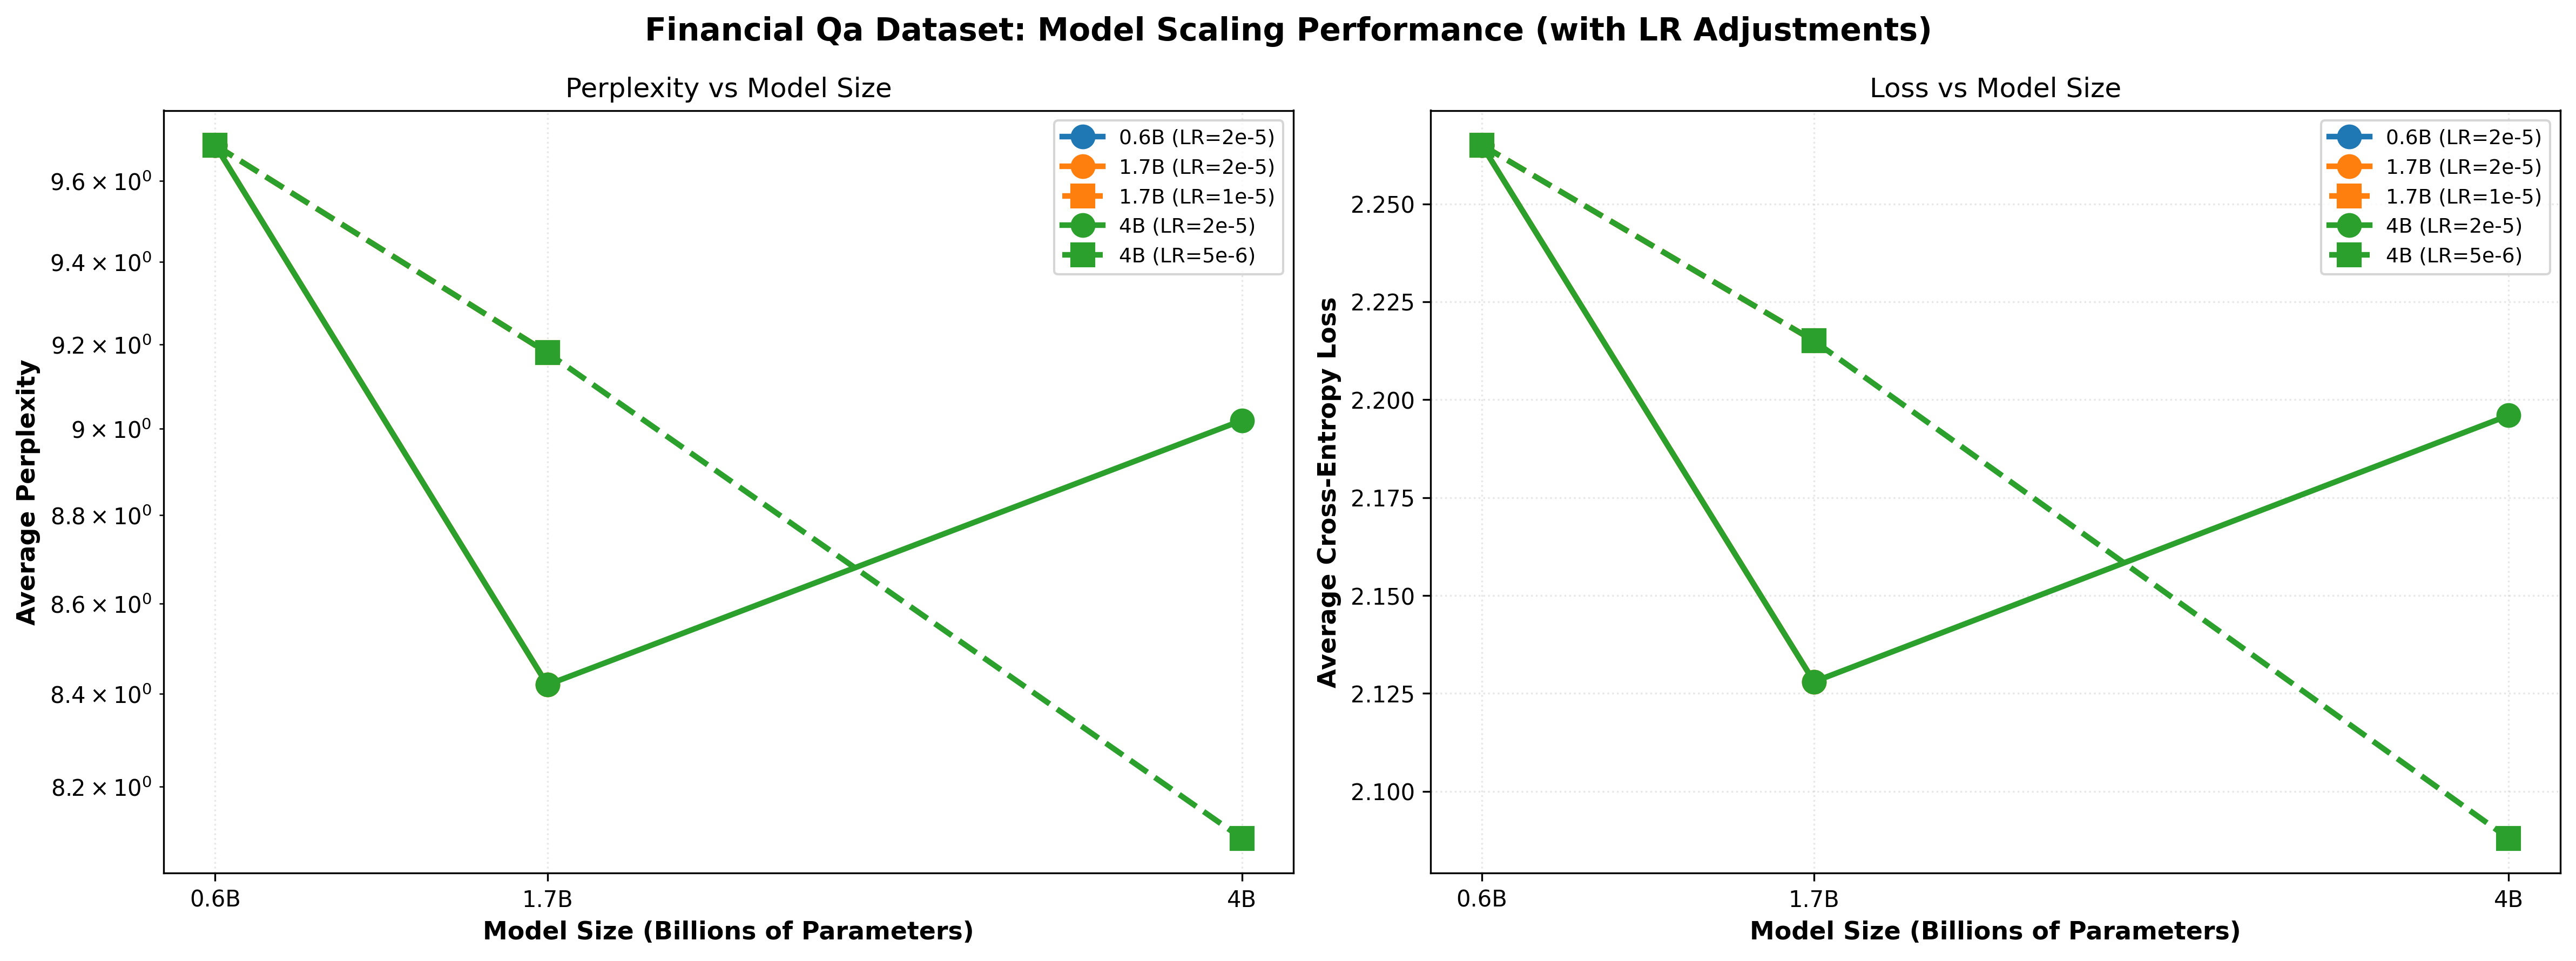
\includegraphics[width=0.9\textwidth]{figures/scaling_financial_qa.png}
\caption[Financial QA 10K Dataset: Reverse Scaling]{Financial QA 10K Dataset: Moderate reverse scaling resolved via learning rate adjustment. The 4B model (dashed line, squares) shows adjusted LR results with 10.4\% improvement, recovering expected scaling order. Extreme overtraining (143 epochs) causes 19.92\% cross-dataset variance.}
\label{fig:scaling_financial_qa}
\end{figure}

\begin{figure}[htbp]
\centering
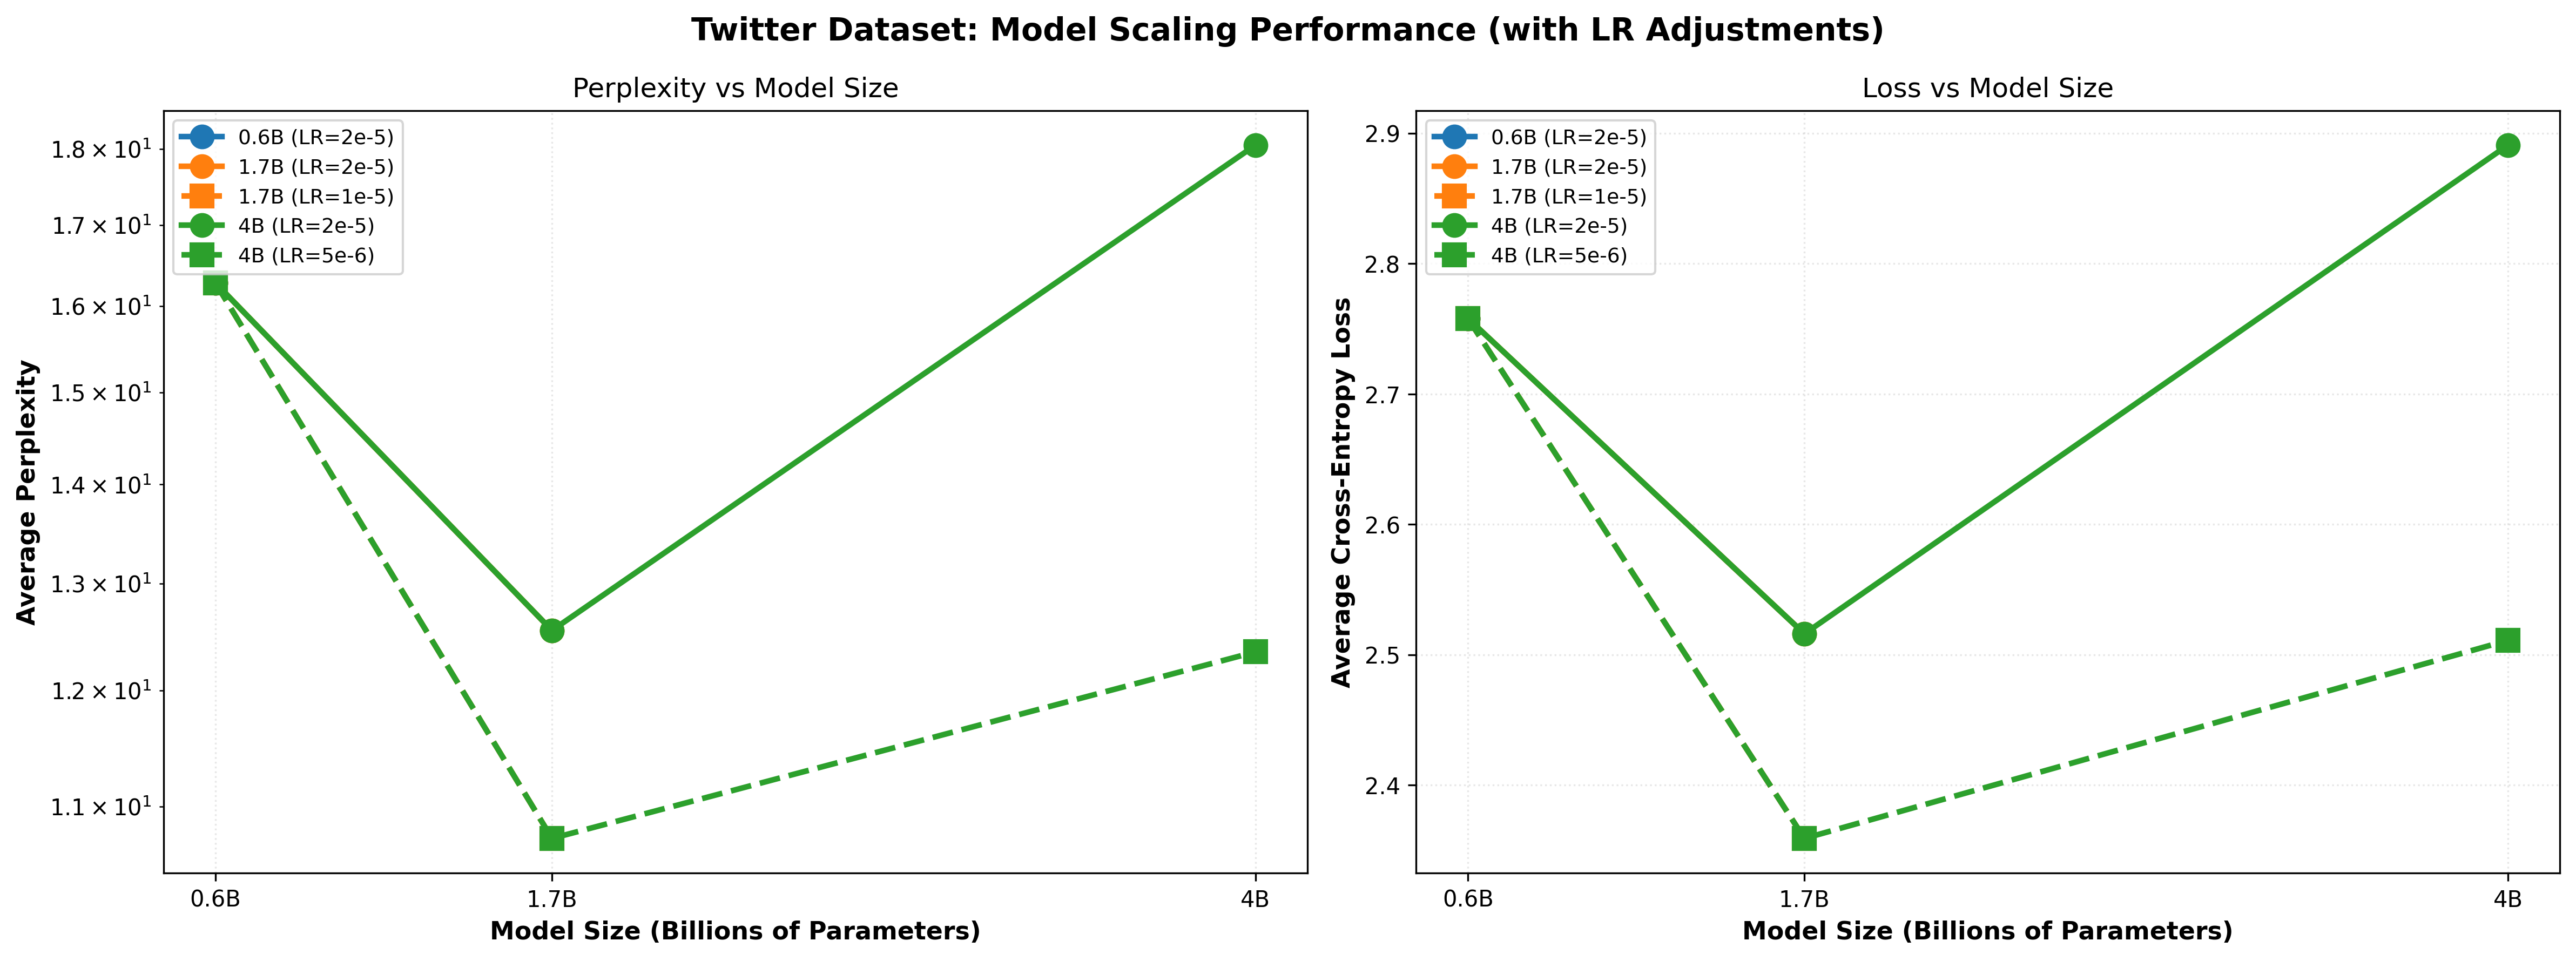
\includegraphics[width=0.9\textwidth]{figures/scaling_twitter.png}
\caption[Twitter Financial Sentiment Dataset: Reverse Scaling]{Twitter Financial Sentiment Dataset: Severe reverse scaling phenomenon. The 4B model (dashed line, squares) required 75\% LR reduction to recover performance, achieving 33.8\% improvement. Extremely small dataset (0.28M tokens, 352 epochs) creates brittle optimization landscape with 20.35\% variance.}
\label{fig:scaling_twitter}
\end{figure}

% Financial QA 10K Dataset: Evaluation Results with LR Adjustments
% Training: Financial QA 10K (virattt/financial-qa-10K, 3.5M tokens)
% LR Adjustments: 1.7B (2e-5 → 1e-5), 4B (2e-5 → 5e-6)

\begin{table}[h]
\centering
\caption[Financial QA 10K: Learning Rate Comparison]{Financial QA 10K Dataset: Impact of Learning Rate Adjustments}
\label{tab:financial_qa_lr_comparison}
\begin{tabular}{l|c|cc|cc|c|cc|cc}
\hline
\multirow{3}{*}{\textbf{Eval Dataset}} &
\multicolumn{5}{c|}{\textbf{Cross-Entropy Loss}} &
\multicolumn{5}{c}{\textbf{Perplexity}} \\
\cline{2-6} \cline{7-11}
& \textbf{0.6B} & \multicolumn{2}{c|}{\textbf{1.7B}} & \multicolumn{2}{c|}{\textbf{4B}} &
 \textbf{0.6B} & \multicolumn{2}{c|}{\textbf{1.7B}} & \multicolumn{2}{c}{\textbf{4B}} \\
\cline{3-4} \cline{5-6} \cline{8-9} \cline{10-11}
& \textbf{2e-5} & \textbf{2e-5} & \textbf{1e-5} & \textbf{2e-5} & \textbf{5e-6} &
 \textbf{2e-5} & \textbf{2e-5} & \textbf{1e-5} & \textbf{2e-5} & \textbf{5e-6} \\
\hline
 Alpaca & 2.38 & \textbf{2.23} & 2.29 & 2.29 & \textbf{2.18} & 10.82 & \textbf{9.31} & 9.92 & \textbf{9.91} & \textbf{8.88} \\
Financial News & 2.36 & \textbf{2.17} & 2.23 & 2.13 & \textbf{2.04} & 10.60 & \textbf{8.78} & 9.25 & \textbf{8.41} & \textbf{7.71} \\
\rowcolor{gray!20} \textbf{Financial QA (train)} & 2.12 & \textbf{2.01} & 2.12 & 2.12 & \textbf{2.01} & 8.29 & \textbf{7.44} & 8.29 & 8.29 & \textbf{7.43} \\
SEC Reports & 2.11 & \textbf{2.00} & 2.10 & 2.11 & \textbf{2.01} & 8.21 & \textbf{7.40} & 8.19 & \textbf{8.25} & \textbf{7.43} \\
FinGPT & 2.31 & \textbf{2.15} & 2.25 & 2.23 & \textbf{2.11} & 10.04 & \textbf{8.62} & 9.51 & \textbf{9.34} & \textbf{8.24} \\
FiQA & 2.40 & \textbf{2.25} & 2.31 & 2.31 & \textbf{2.19} & 11.02 & \textbf{9.45} & 10.10 & \textbf{10.05} & \textbf{8.93} \\
Twitter & 2.21 & \textbf{2.10} & 2.21 & 2.20 & \textbf{2.09} & 9.14 & \textbf{8.18} & 9.10 & \textbf{8.99} & \textbf{8.05} \\
Wikitext & 2.24 & \textbf{2.11} & 2.21 & 2.19 & \textbf{2.08} & 9.41 & \textbf{8.23} & 9.08 & \textbf{8.89} & \textbf{8.00} \\
\rowcolor{blue!10} \textbf{Average} & \textbf{2.27} & \textbf{2.13} & \textbf{2.21} & \textbf{2.20} & \textbf{2.09} & \textbf{9.69} & \textbf{8.42} & \textbf{9.18} & \textbf{9.02} & \textbf{8.09}  \\
\hline
\end{tabular}
\end{table}


% Twitter Financial Dataset: Evaluation Results with LR Adjustments
% Training: Twitter Financial (Financial tweets, 0.28M tokens)
% LR Adjustments: 1.7B (2e-5 → 1e-5), 4B (2e-5 → 5e-6)

\begin{table}[h]
\centering
\caption[Twitter Financial: Learning Rate Comparison]{Twitter Financial Dataset: Impact of Learning Rate Adjustments}
\label{tab:twitter_lr_comparison}
\begin{tabular}{l|c|cc|cc|c|cc|cc}
\hline
\multirow{3}{*}{\textbf{Eval Dataset}} &
\multicolumn{5}{c|}{\textbf{Cross-Entropy Loss}} &
\multicolumn{5}{c}{\textbf{Perplexity}} \\
\cline{2-6} \cline{7-11}
& \textbf{0.6B} & \multicolumn{2}{c|}{\textbf{1.7B}} & \multicolumn{2}{c|}{\textbf{4B}} &
 \textbf{0.6B} & \multicolumn{2}{c|}{\textbf{1.7B}} & \multicolumn{2}{c}{\textbf{4B}} \\
\cline{3-4} \cline{5-6} \cline{8-9} \cline{10-11}
& \textbf{2e-5} & \textbf{2e-5} & \textbf{1e-5} & \textbf{2e-5} & \textbf{5e-6} &
 \textbf{2e-5} & \textbf{2e-5} & \textbf{1e-5} & \textbf{2e-5} & \textbf{5e-6} \\
\hline
 Alpaca & 3.01 & 2.66 & \textbf{2.54} & 2.96 & \textbf{2.61} & 20.21 & 14.33 & \textbf{12.66} & \textbf{19.20} & \textbf{13.65} \\
Financial News & 3.17 & 2.80 & \textbf{2.65} & 2.87 & \textbf{2.54} & 23.77 & 16.48 & \textbf{14.10} & \textbf{17.67} & \textbf{12.68} \\
Financial QA & 2.46 & 2.32 & \textbf{2.16} & 2.83 & \textbf{2.43} & 11.76 & 10.15 & \textbf{8.69} & \textbf{16.98} & \textbf{11.39} \\
SEC Reports & 2.48 & 2.32 & \textbf{2.16} & 2.80 & \textbf{2.39} & 11.95 & 10.17 & \textbf{8.70} & \textbf{16.42} & \textbf{10.93} \\
FinGPT & 2.74 & 2.50 & \textbf{2.34} & 2.91 & \textbf{2.54} & 15.53 & 12.23 & \textbf{10.41} & \textbf{18.34} & \textbf{12.69} \\
FiQA & 2.98 & 2.66 & \textbf{2.50} & 3.00 & \textbf{2.61} & 19.67 & 14.26 & \textbf{12.20} & \textbf{20.09} & \textbf{13.61} \\
\rowcolor{gray!20} \textbf{Twitter (train)} & 2.53 & 2.40 & \textbf{2.22} & 2.88 & \textbf{2.47} & 12.60 & 11.02 & \textbf{9.21} & 17.83 & \textbf{11.81} \\
Wikitext & 2.69 & 2.47 & \textbf{2.30} & 2.88 & \textbf{2.49} & 14.74 & 11.78 & \textbf{9.94} & \textbf{17.85} & \textbf{12.02} \\
\rowcolor{blue!10} \textbf{Average} & \textbf{2.76} & \textbf{2.52} & \textbf{2.36} & \textbf{2.89} & \textbf{2.51} & \textbf{16.28} & \textbf{12.55} & \textbf{10.74} & \textbf{18.05} & \textbf{12.35}  \\
\hline
\end{tabular}
\end{table}



\section{Training Dynamics and Scaling Behavior}

Beyond data mixture effects, our experiments revealed critical insights about model scaling behavior and hyperparameter sensitivity. We observed two distinct scaling patterns across our 10 experiments: normal scaling (larger models consistently outperform smaller ones) and reverse scaling (larger models underperform), with the latter partially resolved through systematic learning rate adjustment.

\subsection{Normal Scaling Pattern}

Seven of ten experiments exhibited expected scaling behavior where larger models achieve lower perplexity than smaller models, consistent with established scaling laws.

\textbf{FiQA (3.6M tokens)}: Clean scaling across all model sizes. 0.6B: 83.57 ppl, 1.7B: 13.47 ppl (83.9\% improvement), 4B: 6.80 ppl (49.5\% improvement over 1.7B, 91.9\% total improvement over 0.6B). The conversational Q\&A format and moderate dataset size provided stable training signals for all scales.

\textbf{FinGPT Sentiment (4.1M tokens)}: Strong scaling with accelerating gains. 0.6B: 35.48 ppl, 1.7B: 11.27 ppl (68.2\% improvement), 4B: 7.03 ppl (37.6\% improvement, 80.2\% total). The instruction-following format benefited particularly from increased model capacity.

\textbf{News Articles (194M tokens)}: Excellent scaling with large improvements. 0.6B: 126.3 ppl, 1.7B: 41.79 ppl (66.9\% improvement), 4B: 32.82 ppl (21.5\% improvement, 74.0\% total). Large dataset size (194M tokens) provided sufficient diversity to fully utilize larger model capacity without overfitting.

\textbf{SEC Reports (8.1M tokens)}: Consistent improvements across scales. 0.6B: 47.46 ppl, 1.7B: 22.18 ppl (53.3\% improvement), 4B: 17.80 ppl (19.7\% improvement, 62.5\% total). The formal, structured nature of regulatory filings created predictable patterns that larger models captured effectively.

\textbf{Finance Alpaca (8.5M tokens)}: Moderate but consistent scaling. 0.6B: 91.37 ppl, 1.7B: 17.90 ppl (80.4\% improvement), 4B: 8.73 ppl (51.2\% improvement, 90.4\% total). Instruction-formatted educational Q\&A showed reliable scaling despite moderate dataset size.

\textbf{Mixed Financial (220M tokens)}: Consistent scaling across model sizes. 0.6B: 130.3 ppl, 1.7B: 34.49 ppl (73.5\% improvement), 4B: 21.55 ppl (37.5\% improvement, 83.5\% total). The diverse 7-dataset mixture showed stable training dynamics with smooth perplexity reduction across scales.

\textbf{Mixed Wiki+Financial (343M tokens)}: Normal scaling maintained despite domain mixture. 0.6B: 75.00 ppl, 1.7B: 38.90 ppl (48.1\% improvement), 4B: 26.69 ppl (31.4\% improvement, 64.4\% total). Smaller relative gains suggest that mixing diverse domains (general + financial) creates competing optimization pressures that partially limit scaling benefits.

\textbf{Pattern Summary}: Normal scaling experiments share key characteristics: (1) dataset size $>$ 4M tokens, (2) stable training loss curves, (3) consistent 62-92\% total perplexity reduction from 0.6B to 4B, (4) larger absolute gains at 0.6B$\to$1.7B than 1.7B$\to$4B (diminishing returns pattern).

\subsection{Reverse Scaling Phenomenon}

Three experiments exhibited \textit{reverse scaling}: larger models performed worse than smaller models with uniform hyperparameters, contradicting standard scaling laws. This phenomenon provided critical insights into hyperparameter sensitivity.

\textbf{WikiText (124M tokens) - Most Severe Case}: 0.6B reached 9.68 ppl (excellent), 1.7B collapsed (infinite loss after epoch 2), and 4B ended at 31.54 ppl after LR adjustment (originally $>$100).

The 0.6B model achieved strong WikiText performance with LR $2\times10^{-5}$, but this same learning rate caused catastrophic instability for 1.7B (gradient explosion, NaN values) and severe degradation for 4B. The clean, structured nature of WikiText may amplify learning rate sensitivity; uniform, high-quality text produces consistent gradients that accumulate more rapidly in larger models.

\textbf{Financial QA 10K (0.7M tokens) - Moderate Reverse Scaling}: 0.6B: 9.69 ppl; 1.7B: 8.42 (13.1\% better); 4B: 9.02 (7.1\% worse than 1.7B; reverse scaling).

The 4B model underperformed despite greater capacity. Small dataset size (0.7M tokens, 143 epochs) combined with technical document complexity created optimization challenges. After LR adjustment to $5\times10^{-6}$, 4B achieved 8.09 ppl (10.3\% improvement), finally surpassing 1.7B and establishing expected scaling order.

\textbf{Twitter Sentiment (0.28M tokens) - Severe Reverse Scaling}: 0.6B: 16.28 ppl; 1.7B: 12.55 (22.9\% better); 4B: 18.05 (43.8\% worse than 1.7B).

Twitter exhibited the most severe reverse scaling among all datasets, with the 4B model performing 43.8\% worse than 1.7B despite improved scaling from 0.6B to 1.7B. The extremely small dataset (0.28M tokens, 352 epochs of overtraining) combined with Twitter's unique distributional characteristics (280-character constraint, informal language, abbreviations) created an exceptionally brittle optimization landscape that amplified learning rate sensitivity at larger scales. Reducing LR to $5\times10^{-6}$ for 4B recovered performance to 12.35 ppl (31.6\% improvement from 18.05), closely approaching 1.7B performance (12.55 ppl). This demonstrates that reverse scaling in our experiments reflects hyperparameter mismatch rather than fundamental model limitations.

\textbf{Root Cause Analysis}: All three reverse‑scaling cases share two properties: (1) problematic learning rate for larger models and (2) either very clean data (WikiText) or very small datasets (Financial QA, Twitter). Clean or small data creates less noise in gradients, making larger models more sensitive to learning rate. With 4B having 6.7$\times$ more parameters than 0.6B, the same LR produces disproportionately large parameter updates, destabilizing training. This scaling amplification effect means larger models require more conservative learning rates. We show the results in \Cref{fig:scaling_wikitext,fig:scaling_financial_qa,fig:scaling_twitter}.

\subsection{Model Stability Analysis}

Beyond individual experiment performance, we analyze training stability across model sizes using loss curve characteristics and cross-dataset variance.

\textbf{Variance by Model Size}: After proper LR tuning, variance reduction from 0.6B to 4B is highly dataset-dependent. Mixed Financial shows strong reduction (98\% to 55\%, 43.6\% reduction), SEC shows even stronger improvement (38\% to 19\%, 49.2\% reduction), while News shows minimal change (68\% to 66\%, 2.9\% reduction).

This dataset-dependent pattern suggests that variance reduction depends on both model capacity and dataset characteristics (size, diversity, domain coherence). Larger models can learn more stable features when training data provides sufficient signal, but dataset limitations constrain generalization improvements regardless of model size.

\textbf{Small Dataset Scaling Paradox}: Small datasets (Financial QA 0.7M, Twitter 0.28M) exhibit the largest variance reductions with scaling: Twitter drops from 74\% to 20\% (72.4\% reduction), Financial QA from 29\% to 20\% (31.1\% reduction). This exceeds News (68\% to 66\%, 2.9\% reduction), demonstrating that small datasets benefit enormously from larger model capacity. However, they retain moderate absolute variance at 4B (19.92-20.35\%), reflecting data scarcity limits despite optimization gains.

\subsection{Variance Across Model Sizes}

\Cref{fig:bar_variance_06b,fig:bar_variance_17b,fig:bar_variance_4b} show variance across all three model sizes. At 0.6B, all datasets exhibit high variance (28-271\%). WikiText shows catastrophic spread (271\%), while other datasets range from 29\% to 98\%. Medium and small datasets start at similar variance levels (Financial QA 29\%, Twitter 74\%, FiQA 69\%, Alpaca 75\%), making it impossible to predict final performance from initial variance alone.

At 1.7B, differentiation begins. Medium datasets achieve best consistency (FiQA 19\%, Alpaca 27\%), dropping by 50-74\% from 0.6B. Small datasets show strong improvement (Financial QA 24\%, Twitter 50\%), with Twitter reducing variance by 32\%. WikiText collapses to 691\% due to training instability. Mixed Wiki+Fin reduces to 34\%, the lowest among mixtures.

At 4B after LR adjustments, final patterns emerge. Medium datasets dominate best-consistency positions: Alpaca 11.5\%, FiQA 19\%, SEC 19\%. Small datasets converge to moderate variance (Financial QA 20\%, Twitter 20\%) despite extreme overtraining (143 and 352 epochs). WikiText recovers to 53\% after LR fix. Large datasets and mixtures remain at 53-66\%.

Variance reduction rates differ by dataset category. Small datasets show largest percentage reductions (Twitter 72\%, Financial QA 31\%), but end at moderate absolute values. Medium datasets show consistent reductions (SEC 49\%, Alpaca 85\%) and reach lowest final variance. Large datasets show minimal improvement (News 3\%). This demonstrates that model capacity interacts with dataset size in non-linear ways.

\begin{figure}[htbp]
\centering
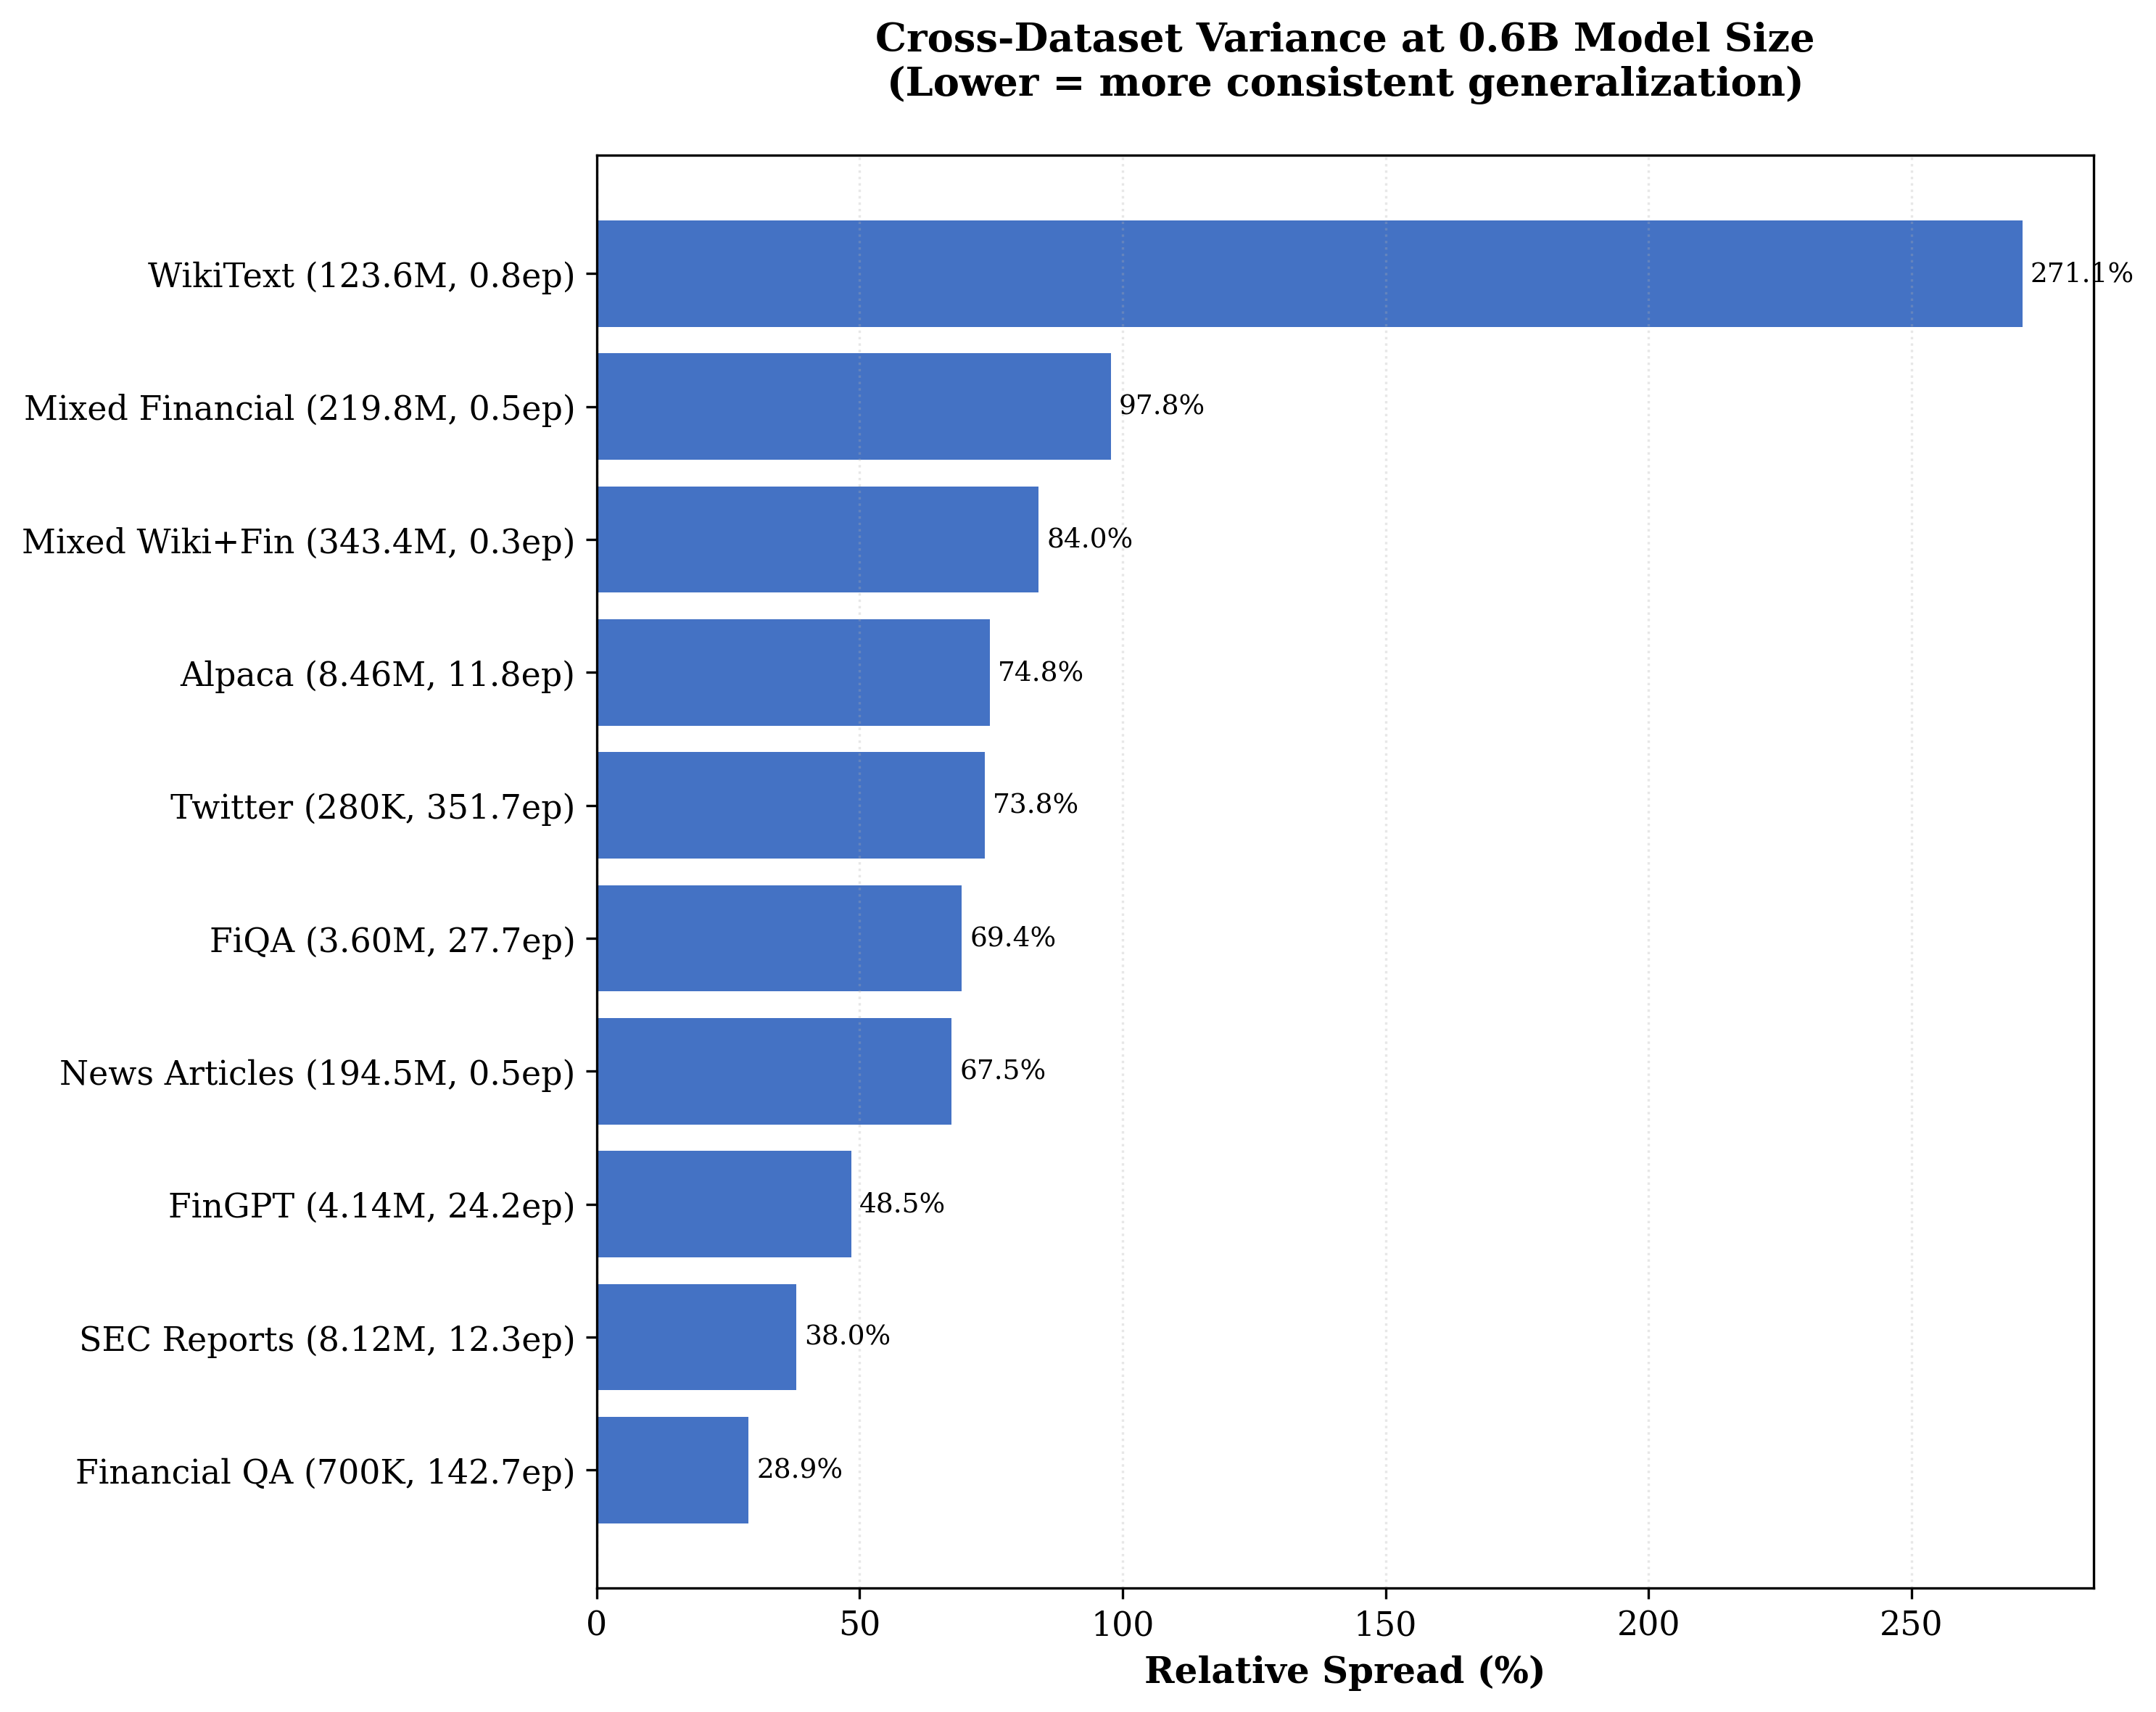
\includegraphics[width=0.85\textwidth]{figures/bar_variance_06b.png}
\caption[Variance at 0.6B Model Size]{Cross-dataset variance at 0.6B model size. All datasets show high variance (28-271\%), with WikiText exhibiting catastrophically high spread (271\%). Small datasets (Twitter 74\%, Financial QA 29\%) and medium datasets (Alpaca 75\%, FiQA 69\%) start with similar variance levels. Mixtures show very high variance (84-98\%). Token counts and epoch counts shown in parentheses.}
\label{fig:bar_variance_06b}
\end{figure}

\begin{figure}[htbp]
\centering
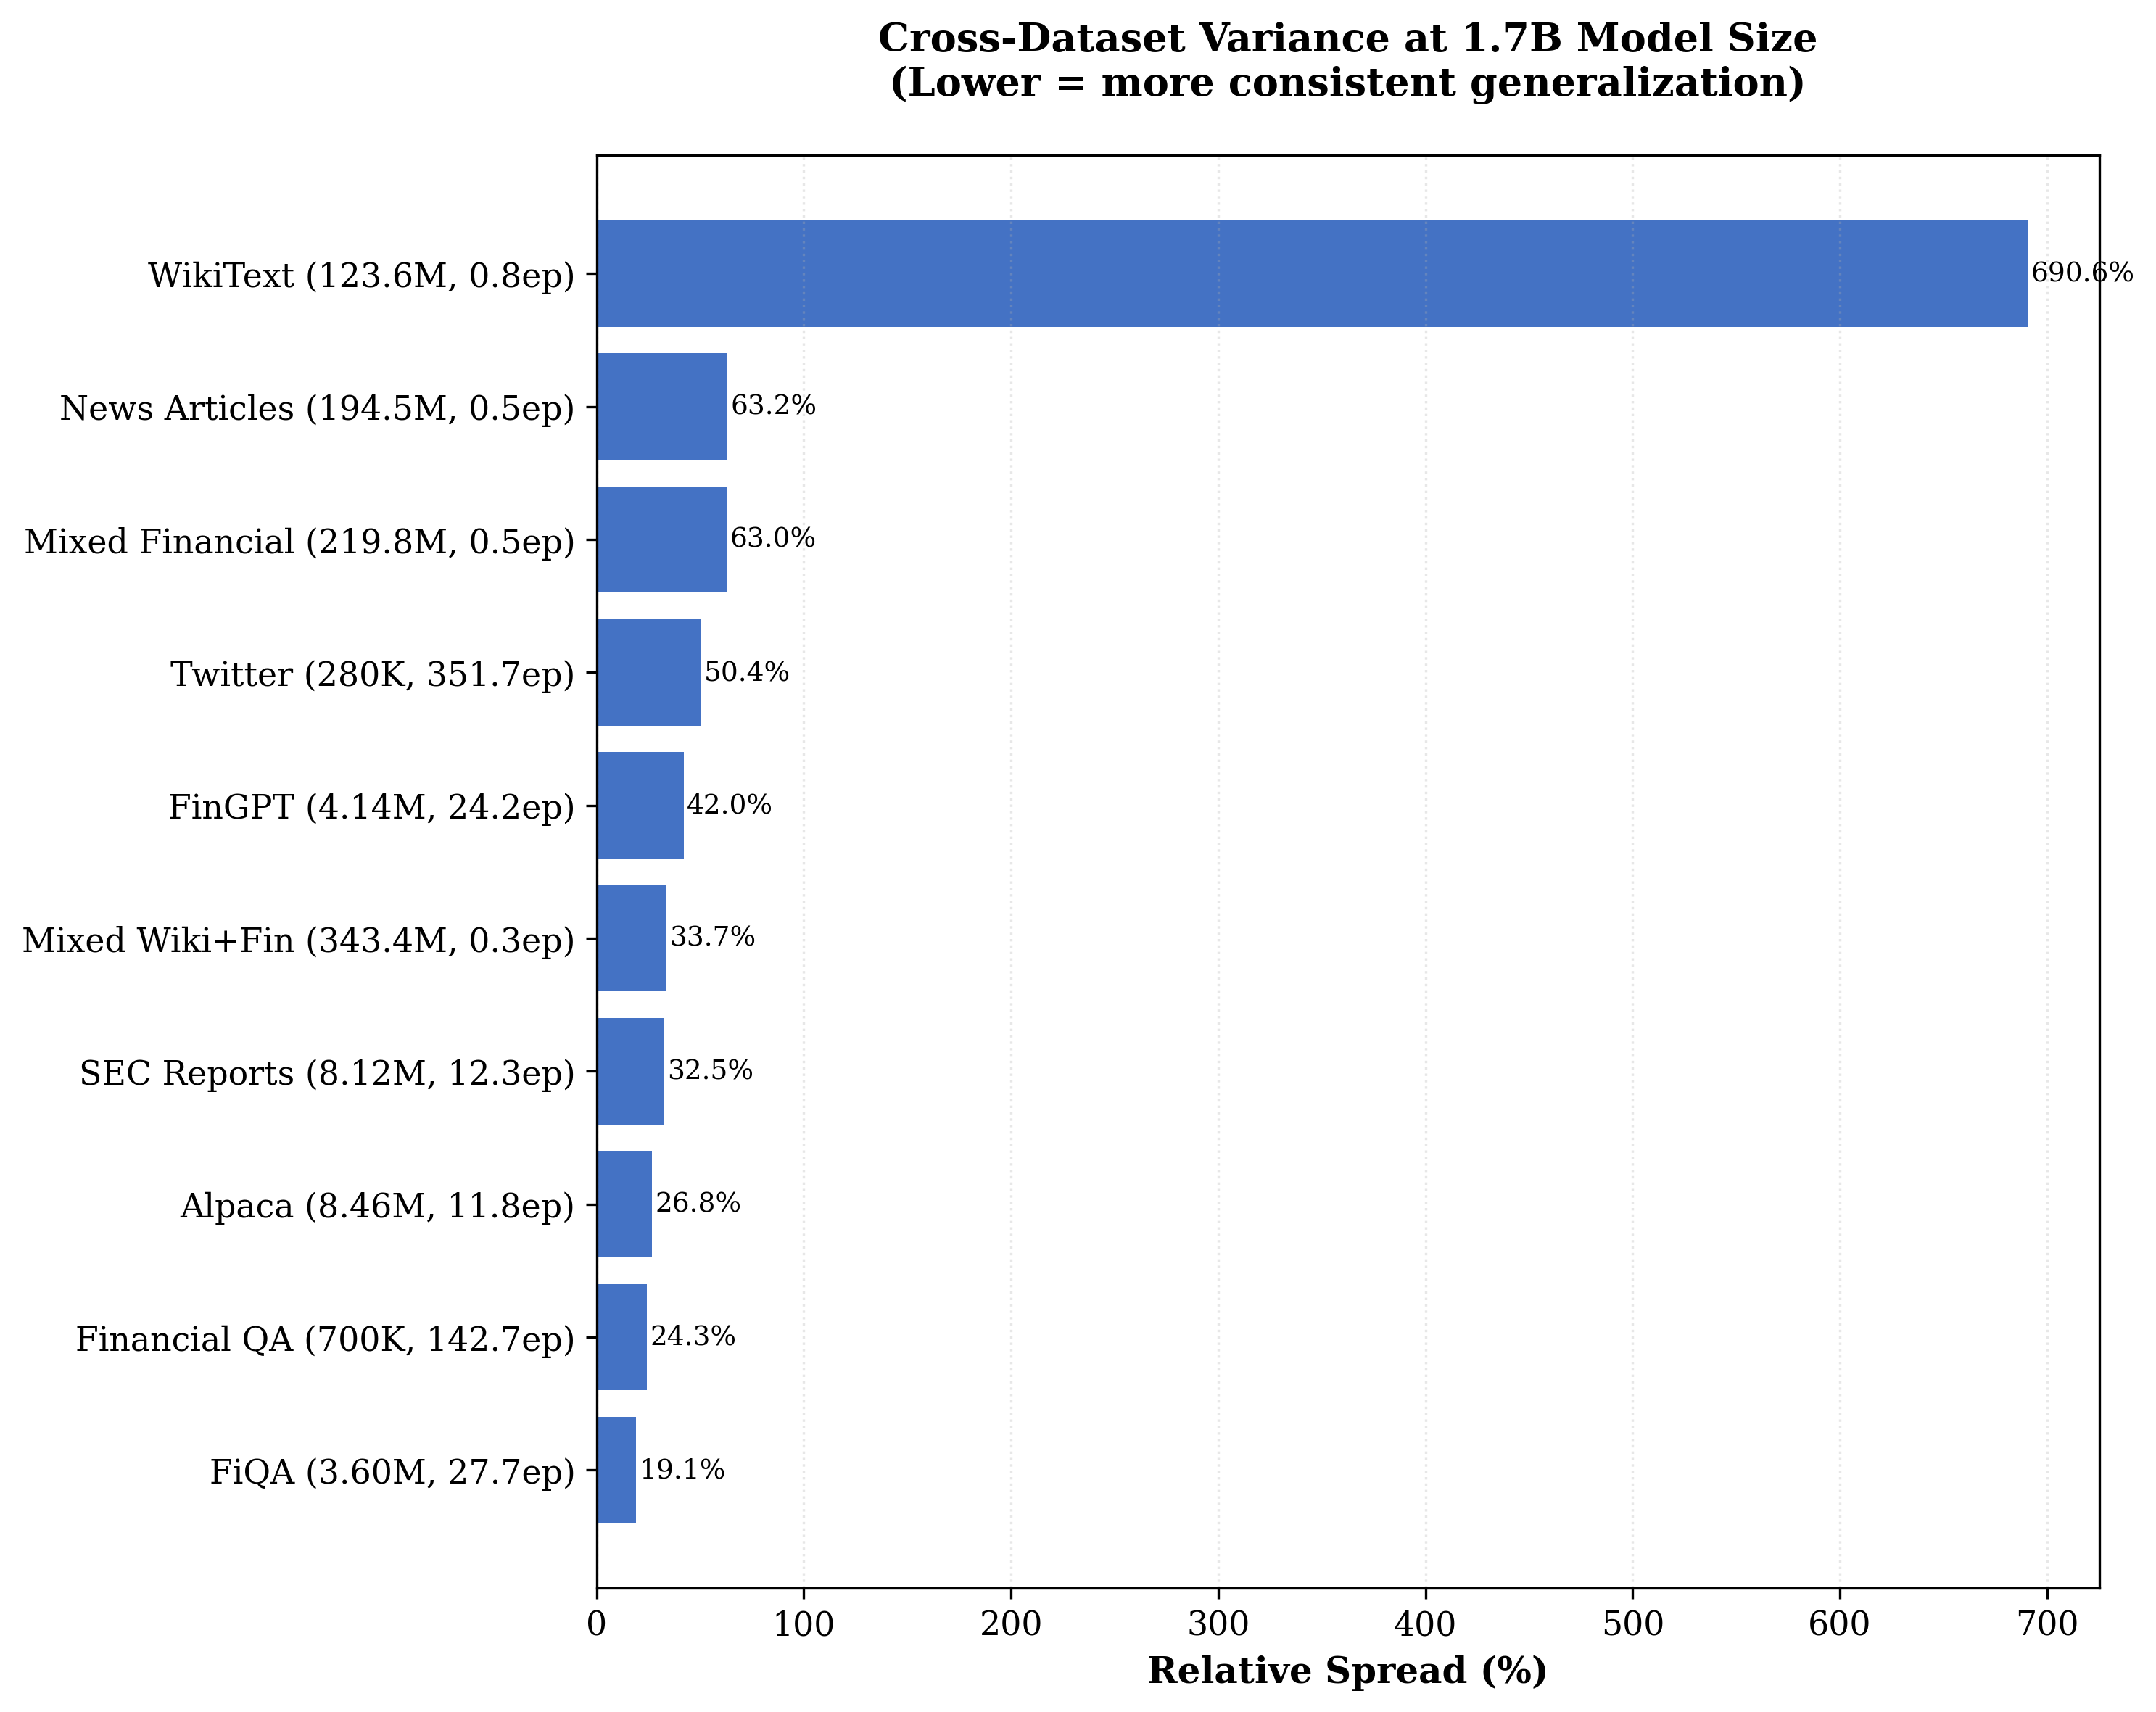
\includegraphics[width=0.85\textwidth]{figures/bar_variance_17b.png}
\caption[Variance at 1.7B Model Size]{Cross-dataset variance at 1.7B model size. Most datasets show substantial variance reduction from 0.6B, except WikiText which collapses with 691\% spread due to training instability. Medium datasets achieve best consistency (FiQA 19\%, Alpaca 27\%), while small datasets show strong improvement (Financial QA 24\%, Twitter 50\%). Mixed Wiki+Fin achieves notable reduction to 34\%.}
\label{fig:bar_variance_17b}
\end{figure}

\begin{figure}[htbp]
\centering
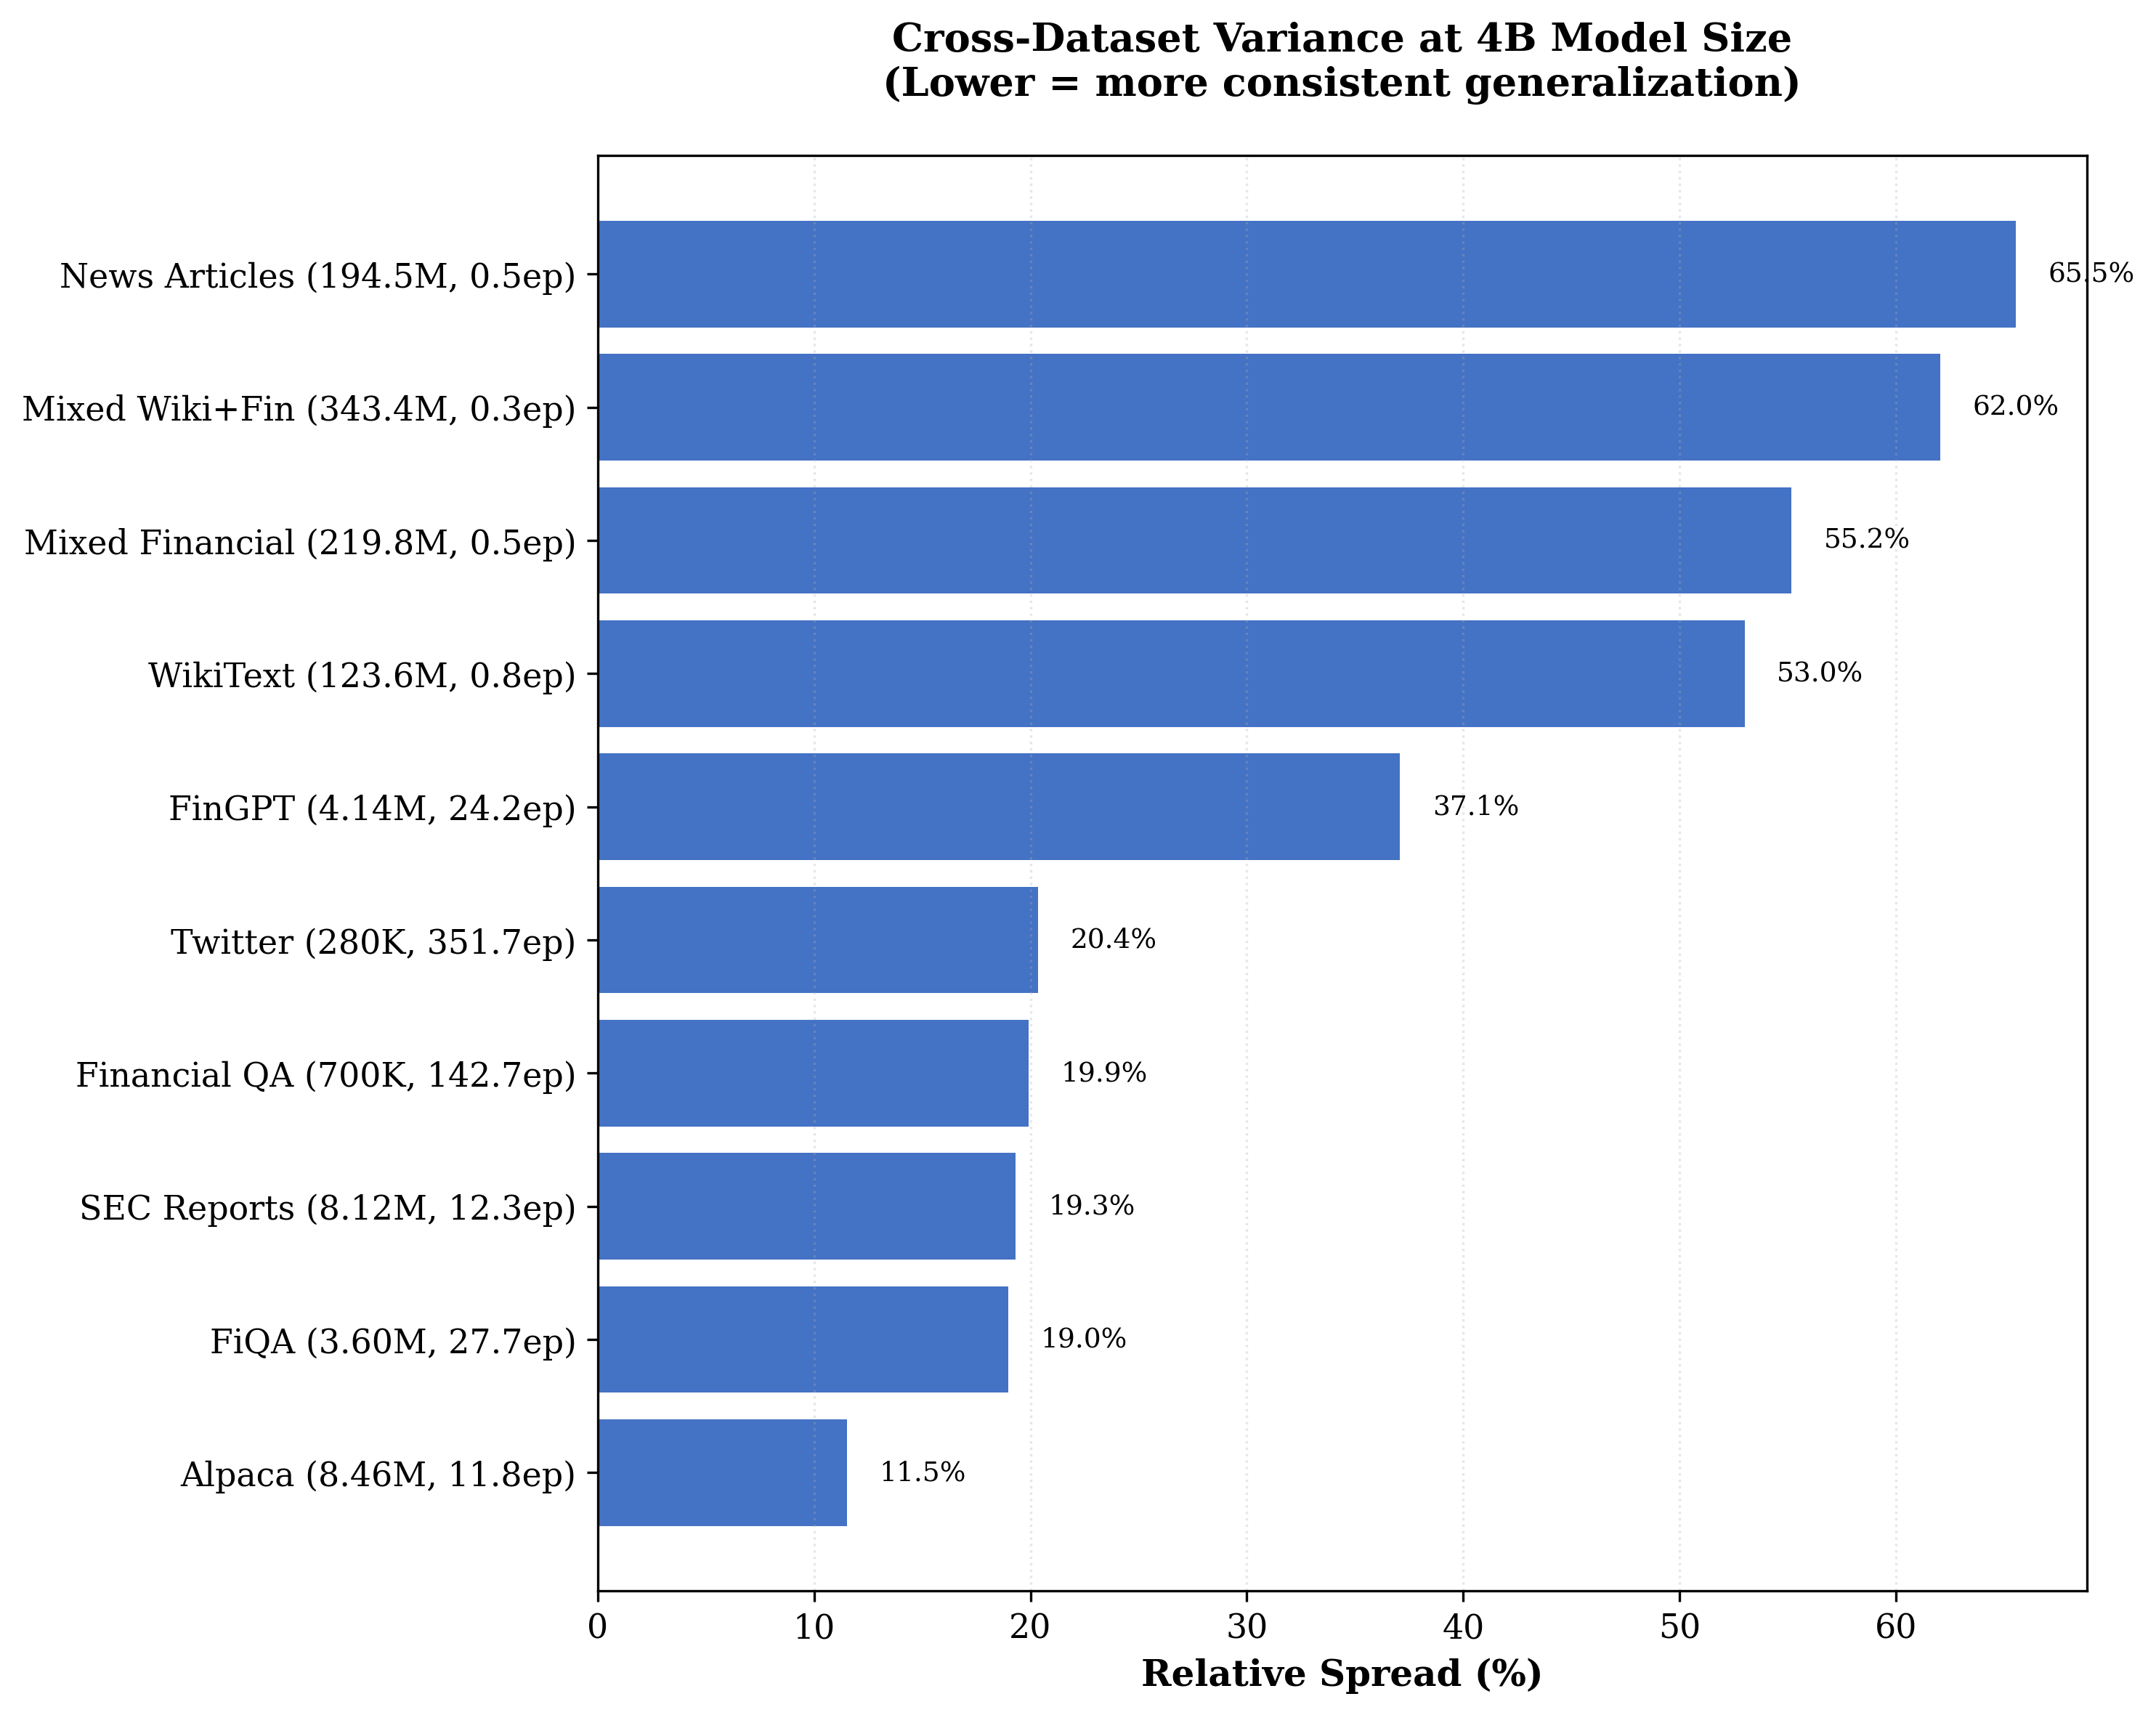
\includegraphics[width=0.85\textwidth]{figures/bar_variance.png}
\caption[Variance at 4B Model Size]{Cross-dataset variance at 4B model size. After LR adjustments, variance continues to decrease for most datasets. Small datasets (Twitter 20\%, Financial QA 20\%) achieve final variance comparable to medium datasets despite extreme overtraining (352ep and 143ep respectively). Medium datasets dominate best-consistency positions (Alpaca 11.5\%, FiQA 19\%, SEC 19\%). WikiText recovers to 53\% after LR fix.}
\label{fig:bar_variance_4b}
\end{figure}

\subsection{Transfer Pattern Analysis}

\Cref{fig:heatmap_transfer_06b,fig:heatmap_transfer_17b,fig:heatmap_transfer} show cross-dataset transfer at 0.6B, 1.7B, and 4B. The rightmost column shows average perplexity across all evaluations, excluding missing data.

At 0.6B, WikiText achieves lowest average transfer (9.7 ppl), followed by Financial QA (9.7 ppl) and Twitter (16.3 ppl). News and mixture configs show poor transfer (75-130 ppl average). All models achieve acceptable performance on most individual datasets (4-30 ppl range) except News and mixtures.

At 1.7B, transfer quality degrades significantly for WikiText. WikiText (2e-5) collapses with 21.3 ppl average, excluding the catastrophic instabilities on evaluating FinQA. WikiText (5e-6) performs worst at 49.9 ppl average. Financial QA maintains best transfer at 8.4-9.2 ppl average. Twitter shows 10.7-12.6 ppl average. The $\infty$ cell indicates training failure (WikiText 2e-5 on Financial QA evaluation).

At 4B after LR adjustments, FinGPT achieves best average transfer (7.0 ppl), followed by FiQA (6.8 ppl) and Alpaca (8.7 ppl). Financial QA averages 8.1-9.0 ppl. Twitter averages 12.3-18.0 ppl. News and mixtures show moderate transfer (21.5-32.8 ppl). Mid-sized datasets (FinGPT, FiQA, Alpaca) achieve consistent single-digit perplexity across all evaluations.

Optimal training configuration shifts across model sizes. At 0.6B, WikiText and small datasets transfer best. At 1.7B, all dataset setups improve on transferability except WikiText. At 4B, mid-sized datasets give the best performance. This pattern aligns with scaling law observations \parencite{kaplan2020scaling,hoffmann2022training}: model capacity must match dataset characteristics and training token budget.

\Cref{tab:cross_financial_news,tab:cross_financial_report,tab:cross_alpaca,tab:cross_fingpt,tab:cross_fiqa,tab:cross_twitter,tab:cross_financial_qa,tab:cross_wikitext} provide detailed cross-dataset comparisons.

\begin{figure}[htbp]
\centering
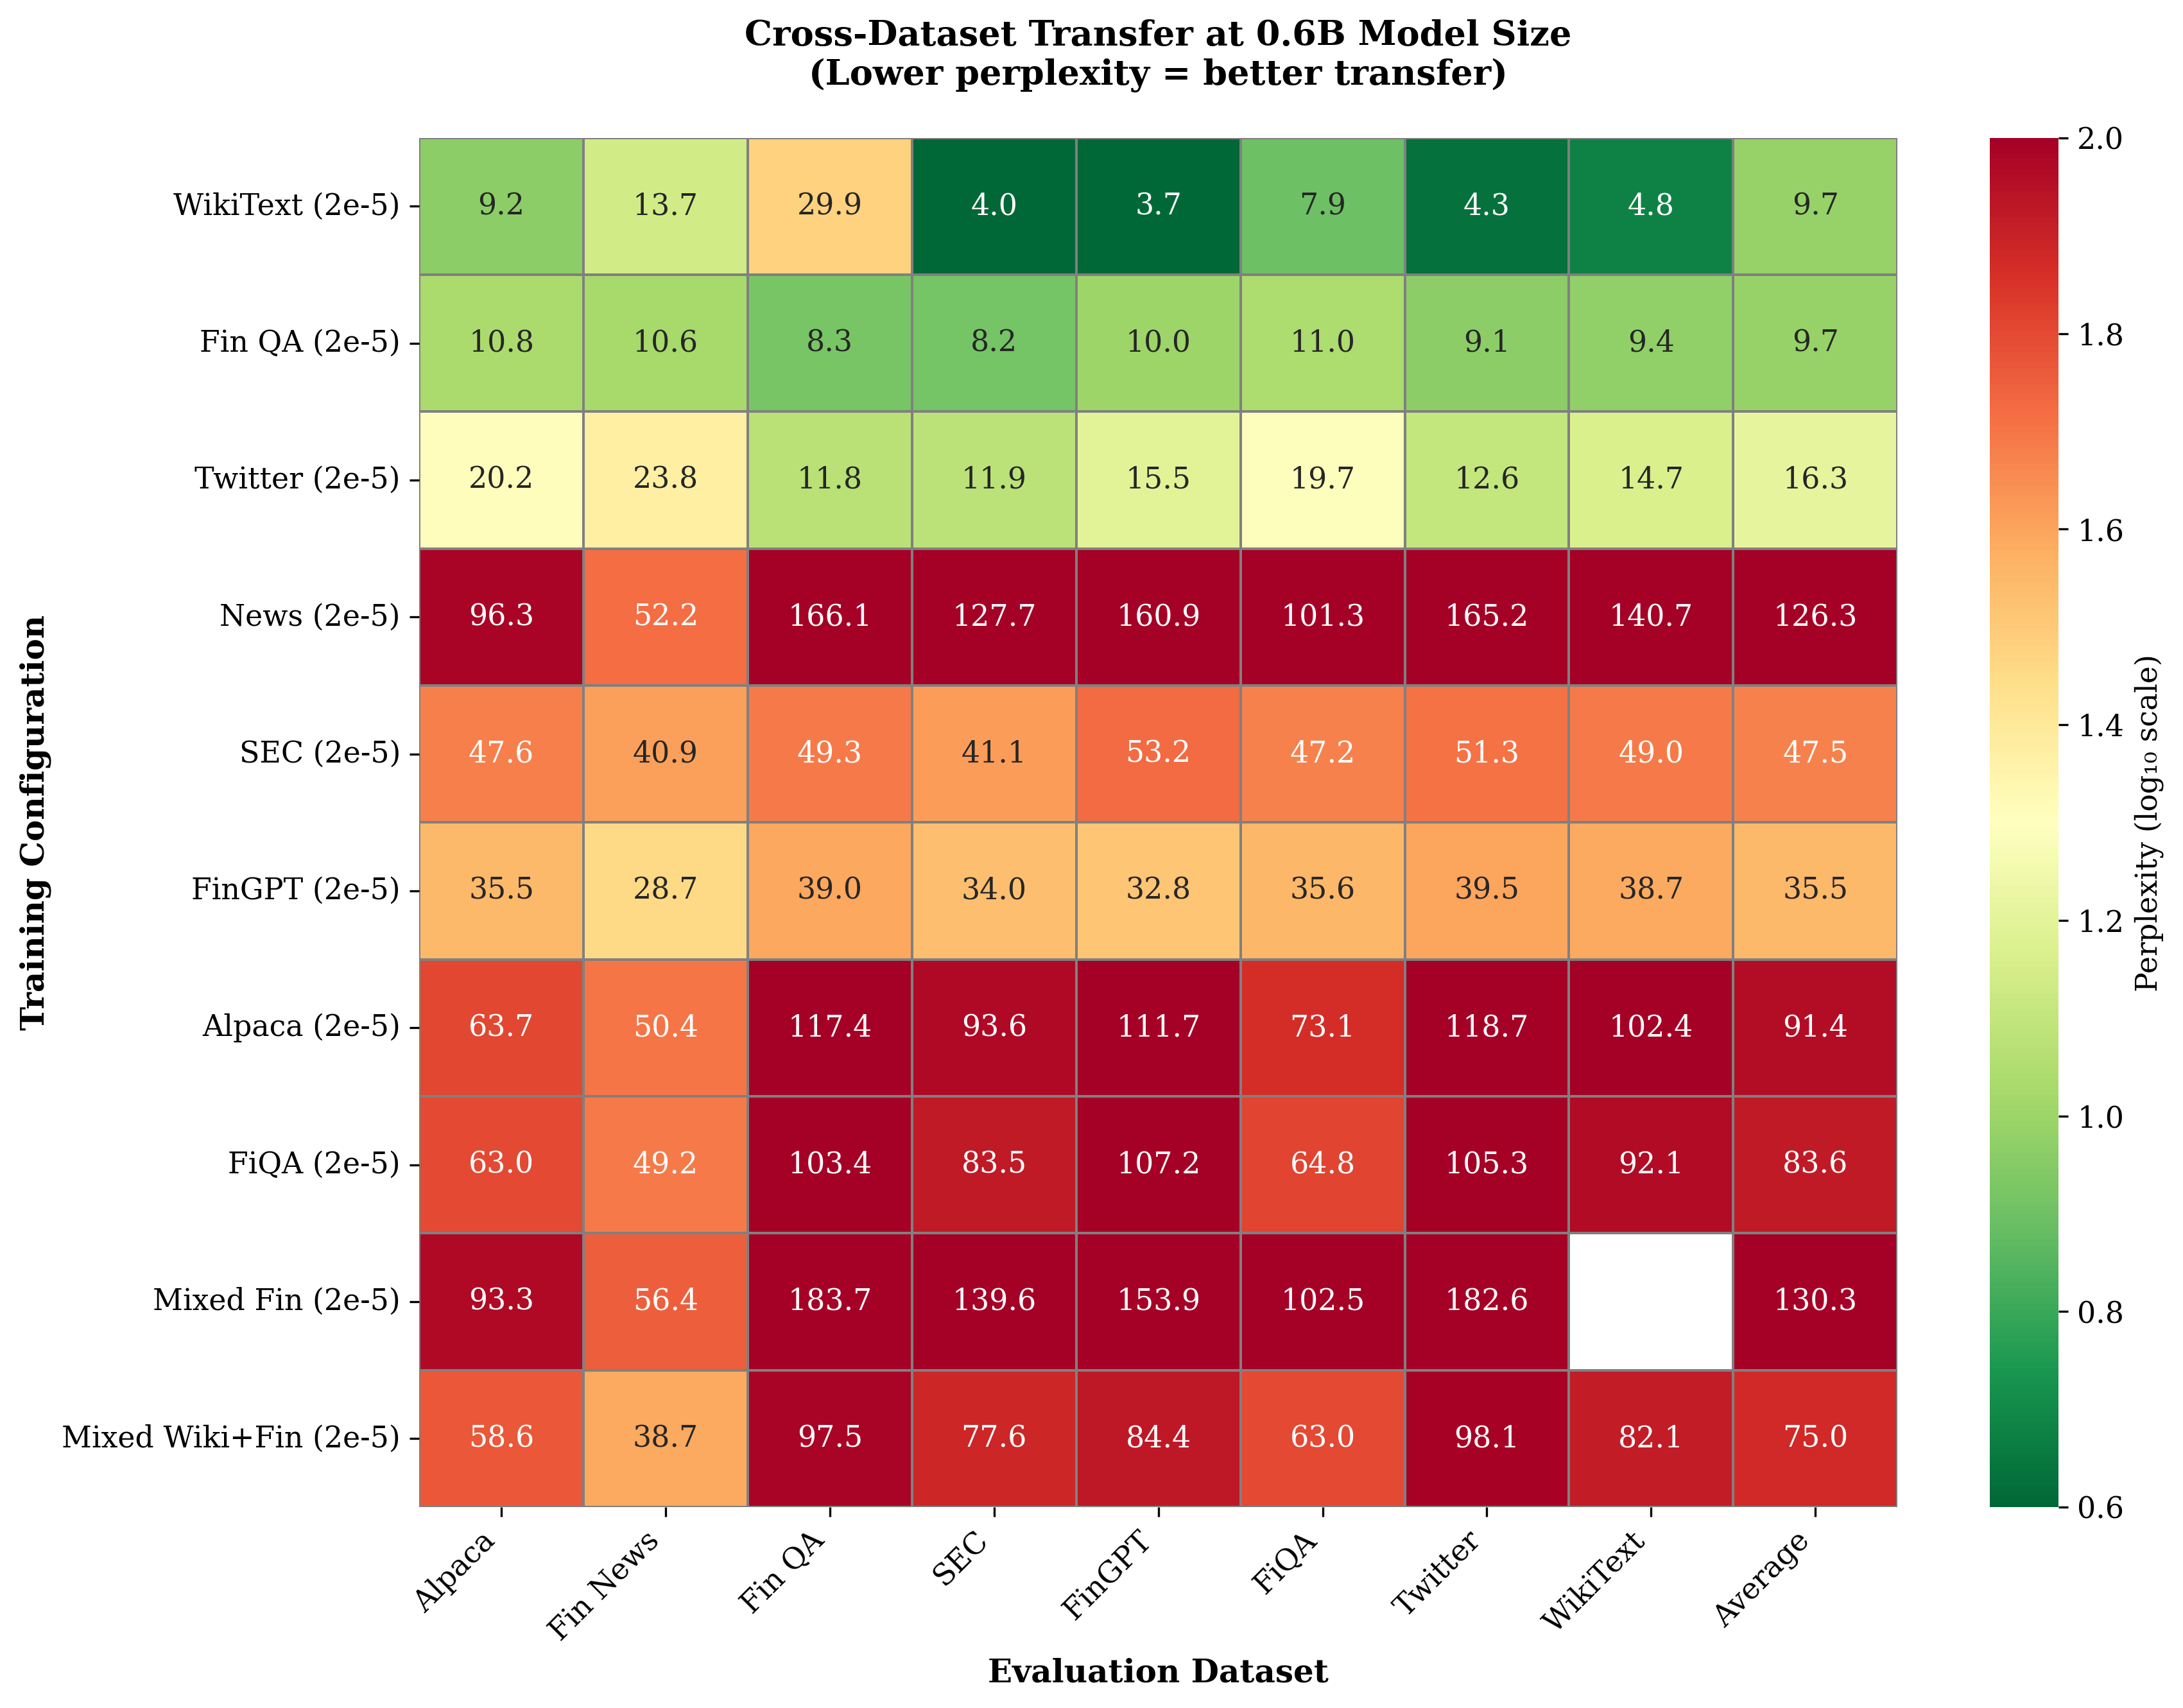
\includegraphics[width=\textwidth]{figures/heatmap_transfer_06b.png}
\caption[Cross-Dataset Transfer at 0.6B]{Cross-dataset transfer at 0.6B.}
\label{fig:heatmap_transfer_06b}
\end{figure}

\begin{figure}[htbp]
\centering
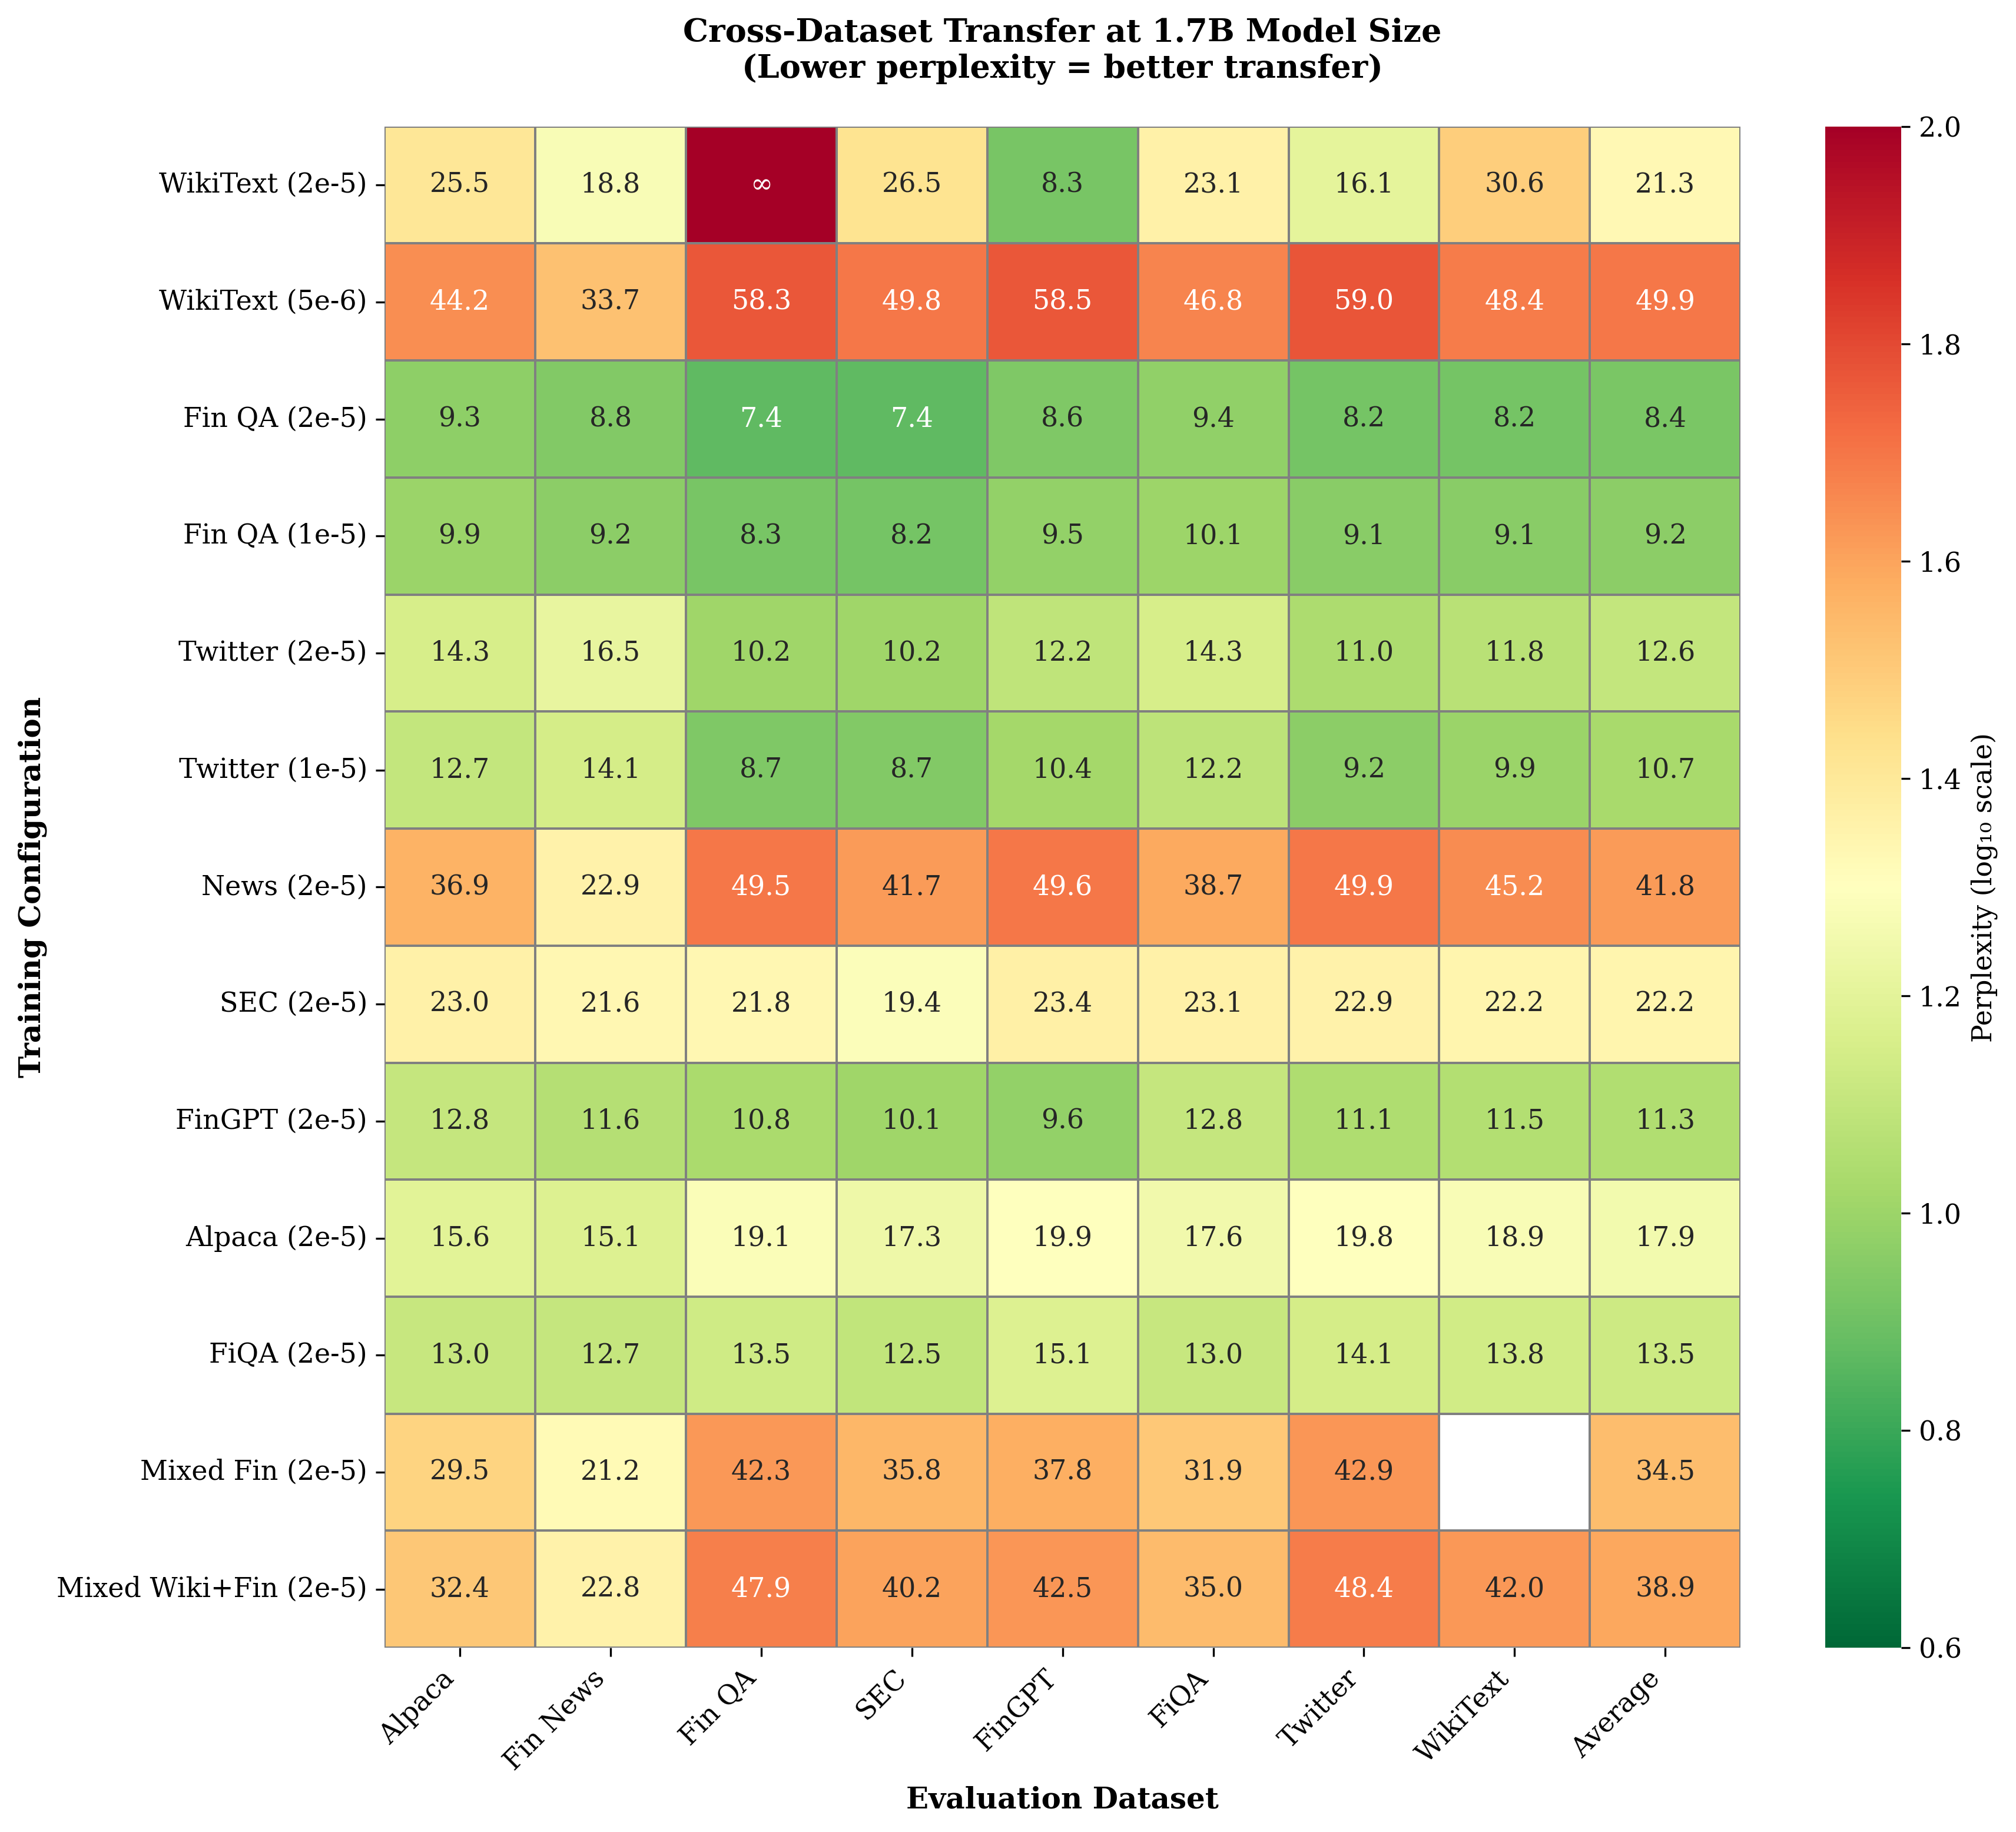
\includegraphics[width=\textwidth]{figures/heatmap_transfer_17b.png}
\caption[Cross-Dataset Transfer at 1.7B]{Cross-dataset transfer at 1.7B.}
\label{fig:heatmap_transfer_17b}
\end{figure}

\begin{figure}[htbp]
\centering
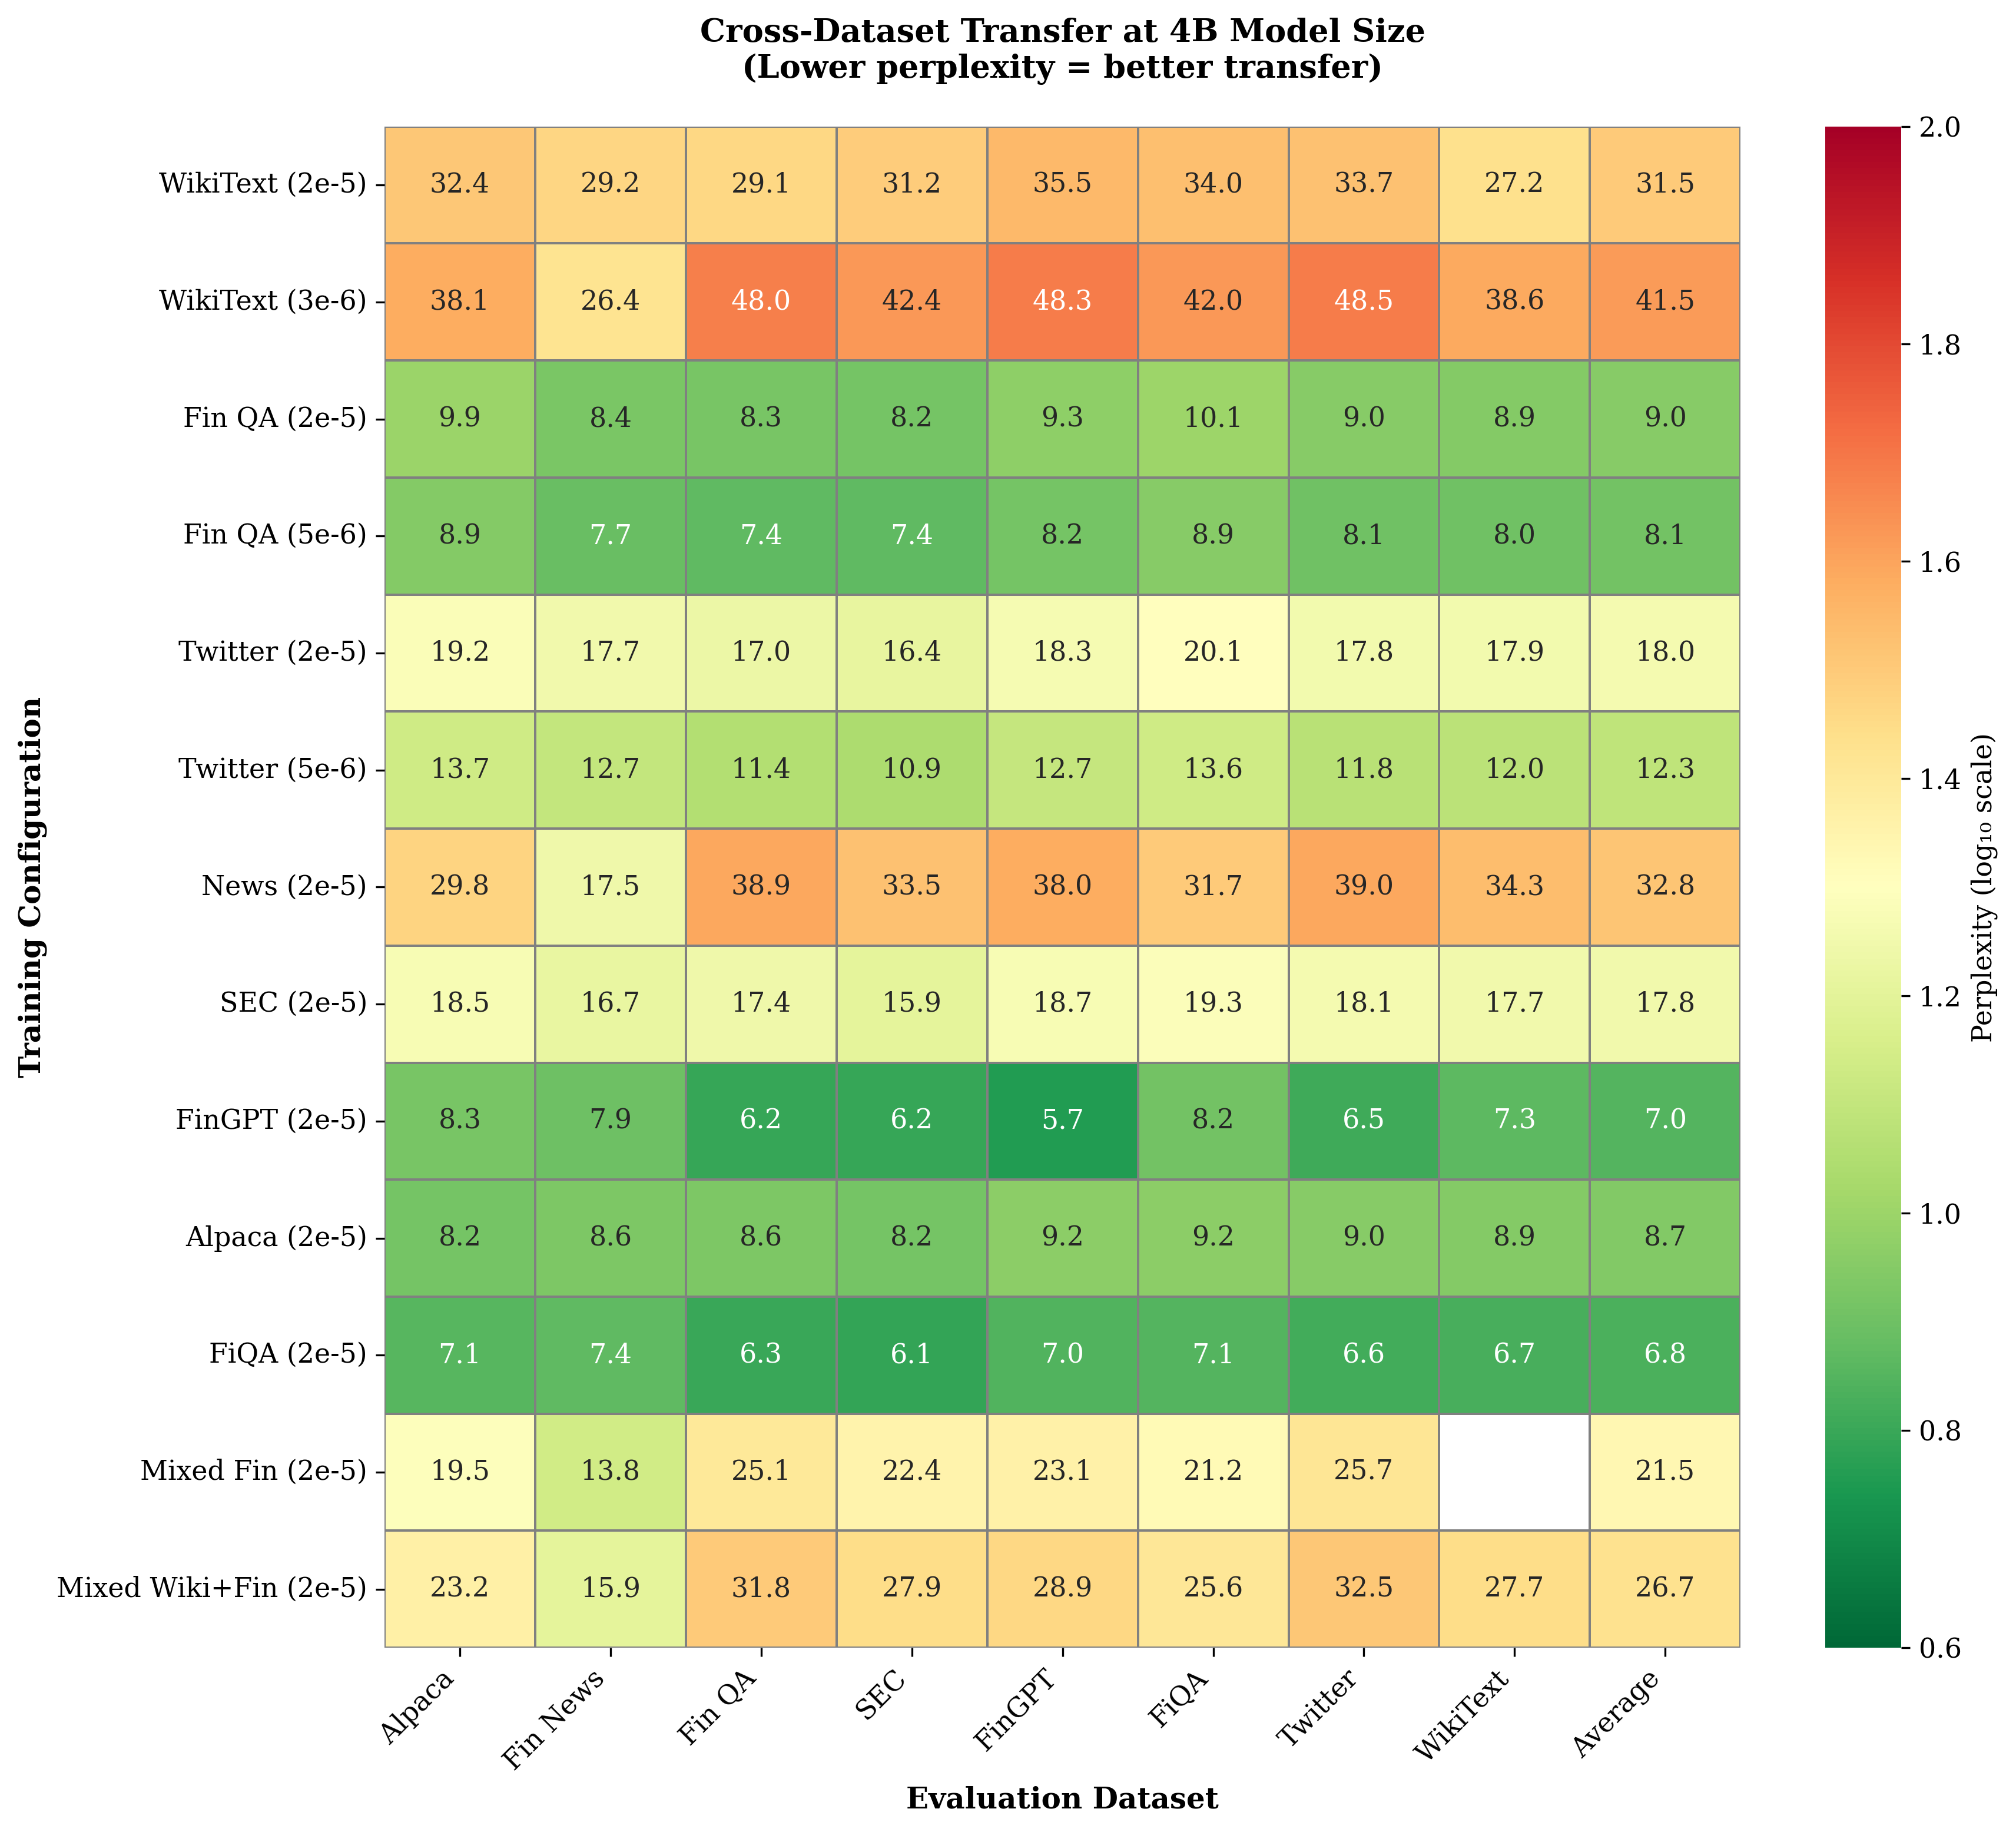
\includegraphics[width=\textwidth]{figures/heatmap_transfer.png}
\caption[Cross-Dataset Transfer at 4B]{Cross-dataset transfer at 4B.}
\label{fig:heatmap_transfer}
\end{figure}

% Cross-Dataset Comparison: Financial News as Evaluation Dataset
% Shows which training dataset performs best on Financial News
% Bold values indicate best performance for each model size

\begin{table}[h]
\centering
\caption{Financial News Evaluation: Performance Across Training Datasets}
\label{tab:cross_financial_news}
\begin{tabular}{l|ccc|ccc}
\hline
\textbf{Training Dataset} & \multicolumn{3}{c|}{\textbf{Cross-Entropy Loss}} & \multicolumn{3}{c}{\textbf{Perplexity}} \\n\cline{2-4} \cline{5-7}
  & \textbf{0.6B} & \textbf{1.7B} & \textbf{4B} & \textbf{0.6B} & \textbf{1.7B} & \textbf{4B} \\
Alpaca (2e-5) & 3.92 & 2.71 & 2.15 & 50.40 & 15.05 & 8.58  \
 Financial QA (2e-5) & \textbf{2.36} & \textbf{2.17} & 2.13 & \textbf{10.60} & \textbf{8.78} & 8.41  \
 Financial QA (1.7B: 1e-5, 4B: 5e-6) & \textbf{2.36} & 2.23 & 2.04 & \textbf{10.60} & 9.25 & 7.71  \
 FinGPT (2e-5) & 3.36 & 2.45 & 2.07 & 28.72 & 11.58 & 7.92  \
 FiQA (2e-5) & 3.90 & 2.54 & \textbf{2.01} & 49.22 & 12.74 & \textbf{7.43}  \
 Mixed Financial (2e-5) & 4.03 & 3.05 & 2.63 & 56.35 & 21.19 & 13.84  \
 Mixed Wiki+Financial (2e-5) & 3.65 & 3.13 & 2.77 & 38.68 & 22.79 & 15.91  \
 Financial News (2e-5) & 3.96 & 3.13 & 2.86 & 52.25 & 22.91 & 17.47  \
 SEC Reports (2e-5) & 3.71 & 3.08 & 2.81 & 40.85 & 21.65 & 16.67  \
 Twitter Financial (2e-5) & 3.17 & 2.80 & 2.87 & 23.77 & 16.48 & 17.67  \
 Twitter Financial (1.7B: 1e-5, 4B: 5e-6) & 3.17 & 2.65 & 2.54 & 23.77 & 14.10 & 12.68  \
 WikiText (2e-5) & 2.62 & 2.93 & 3.37 & 13.70 & 18.78 & 29.19  \
 WikiText (1.7B: 5e-6, 4B: 3e-6) & 2.62 & 3.52 & 3.27 & 13.70 & 33.66 & 26.44  \
\hline
\end{tabular}
\end{table}



% Cross-Dataset Comparison: SEC Reports as Evaluation Dataset
% Shows which training dataset performs best on SEC Reports
% Bold values indicate best performance for each model size

\begin{table}[htbp]
\centering
\caption[SEC Reports Evaluation: Cross-Dataset Performance]{SEC Reports Evaluation: Performance Across Training Datasets}
\label{tab:cross_financial_report}
\begin{tabular}{l|ccc|ccc}
\hline
\textbf{Training Dataset} & \multicolumn{3}{c|}{\textbf{Cross-Entropy Loss}} & \multicolumn{3}{c}{\textbf{Perplexity}} \\
\cline{2-4} \cline{5-7}
  & \textbf{0.6B} & \textbf{1.7B} & \textbf{4B} & \textbf{0.6B} & \textbf{1.7B} & \textbf{4B} \\
Alpaca (2e-5) & 4.54 & 2.85 & 2.11 & 93.56 & 17.26 & 8.25  \\
Financial QA (2e-5) & 2.11 & \textbf{2.00} & 2.11 & 8.21 & \textbf{7.40} & 8.25  \\
Financial QA (1.7B: 1e-5, 4B: 5e-6) & 2.11 & 2.10 & 2.01 & 8.21 & 8.19 & 7.43  \\
FinGPT (2e-5) & 3.53 & 2.31 & 1.82 & 33.97 & 10.12 & 6.20  \\
FiQA (2e-5) & 4.42 & 2.53 & \textbf{1.81} & 83.48 & 12.51 & \textbf{6.14}  \\
Mixed Financial (2e-5) & 4.94 & 3.58 & 3.11 & 139.62 & 35.83 & 22.36  \\
Mixed Wiki+Financial (2e-5) & 4.35 & 3.69 & 3.33 & 77.57 & 40.17 & 27.91  \\
Financial News (2e-5) & 4.85 & 3.73 & 3.51 & 127.73 & 41.68 & 33.46  \\
SEC Reports (2e-5) & 3.72 & 2.96 & 2.77 & 41.12 & 19.36 & 15.91  \\
Twitter Financial (2e-5) & 2.48 & 2.32 & 2.80 & 11.95 & 10.17 & 16.42  \\
Twitter Financial (1.7B: 1e-5, 4B: 5e-6) & 2.48 & 2.16 & 2.39 & 11.95 & 8.70 & 10.93  \\
WikiText (2e-5) & \textbf{1.39} & 3.27 & 3.44 & \textbf{3.99} & 26.46 & 31.23  \\
WikiText (1.7B: 5e-6, 4B: 3e-6) & \textbf{1.39} & 3.91 & 3.75 & \textbf{3.99} & 49.83 & 42.41  \\
\hline
\end{tabular}
\end{table}



% Cross-Dataset Comparison: Alpaca as Evaluation Dataset
% Shows which training dataset performs best on Alpaca
% Bold values indicate best performance for each model size

\begin{table}[htbp]
\centering
\caption[Alpaca Evaluation: Cross-Dataset Performance]{Alpaca Evaluation: Performance Across Training Datasets}
\label{tab:cross_alpaca}
\begin{tabular}{l|ccc|ccc}
\hline
\textbf{Training Dataset} & \multicolumn{3}{c|}{\textbf{Cross-Entropy Loss}} & \multicolumn{3}{c}{\textbf{Perplexity}} \\
\cline{2-4} \cline{5-7}
  & \textbf{0.6B} & \textbf{1.7B} & \textbf{4B} & \textbf{0.6B} & \textbf{1.7B} & \textbf{4B} \\
Alpaca (2e-5) & 4.16 & 2.75 & 2.11 & 63.73 & 15.61 & 8.22  \\
Financial QA (2e-5) & 2.38 & \textbf{2.23} & 2.29 & 10.82 & \textbf{9.31} & 9.91  \\
Financial QA (1.7B: 1e-5, 4B: 5e-6) & 2.38 & 2.29 & 2.18 & 10.82 & 9.92 & 8.88  \\
FinGPT (2e-5) & 3.57 & 2.55 & 2.11 & 35.55 & 12.78 & 8.27  \\
FiQA (2e-5) & 4.14 & 2.56 & \textbf{1.96} & 62.97 & 12.96 & \textbf{7.12}  \\
Mixed Financial (2e-5) & 4.54 & 3.38 & 2.97 & 93.35 & 29.53 & 19.50  \\
Mixed Wiki+Financial (2e-5) & 4.07 & 3.48 & 3.15 & 58.56 & 32.38 & 23.23  \\
Financial News (2e-5) & 4.57 & 3.61 & 3.39 & 96.31 & 36.92 & 29.75  \\
SEC Reports (2e-5) & 3.86 & 3.14 & 2.92 & 47.65 & 23.04 & 18.54  \\
Twitter Financial (2e-5) & 3.01 & 2.66 & 2.96 & 20.21 & 14.33 & 19.20  \\
Twitter Financial (1.7B: 1e-5, 4B: 5e-6) & 3.01 & 2.54 & 2.61 & 20.21 & 12.66 & 13.65  \\
WikiText (2e-5) & \textbf{2.22} & 3.24 & 3.48 & \textbf{9.23} & 25.51 & 32.38  \\
WikiText (1.7B: 5e-6, 4B: 3e-6) & \textbf{2.22} & 3.79 & 3.64 & \textbf{9.23} & 44.22 & 38.06  \\
\hline
\end{tabular}
\end{table}



% Cross-Dataset Comparison: FinGPT as Evaluation Dataset
% Shows which training dataset performs best on FinGPT
% Bold values indicate best performance for each model size

\begin{table}[h]
\centering
\caption[FinGPT Evaluation: Cross-Dataset Performance]{FinGPT Evaluation: Performance Across Training Datasets}
\label{tab:cross_fingpt}
\begin{tabular}{l|ccc|ccc}
\hline
\textbf{Training Dataset} & \multicolumn{3}{c|}{\textbf{Cross-Entropy Loss}} & \multicolumn{3}{c}{\textbf{Perplexity}} \\
\cline{2-4} \cline{5-7}
  & \textbf{0.6B} & \textbf{1.7B} & \textbf{4B} & \textbf{0.6B} & \textbf{1.7B} & \textbf{4B} \\
Alpaca (2e-5) & 4.71 & 2.99 & 2.22 & 111.65 & 19.85 & 9.18  \\
Financial QA (2e-5) & 2.31 & 2.15 & 2.23 & 10.04 & 8.62 & 9.34  \\
Financial QA (1.7B: 1e-5, 4B: 5e-6) & 2.31 & 2.25 & 2.11 & 10.04 & 9.51 & 8.24  \\
FinGPT (2e-5) & 3.49 & 2.26 & \textbf{1.74} & 32.78 & 9.56 & \textbf{5.67}  \\
FiQA (2e-5) & 4.67 & 2.71 & 1.95 & 107.25 & 15.08 & 7.01  \\
Mixed Financial (2e-5) & 5.04 & 3.63 & 3.14 & 153.94 & 37.82 & 23.08  \\
Mixed Wiki+Financial (2e-5) & 4.44 & 3.75 & 3.37 & 84.43 & 42.50 & 28.92  \\
Financial News (2e-5) & 5.08 & 3.90 & 3.64 & 160.92 & 49.56 & 38.03  \\
SEC Reports (2e-5) & 3.97 & 3.15 & 2.93 & 53.18 & 23.41 & 18.68  \\
Twitter Financial (2e-5) & 2.74 & 2.50 & 2.91 & 15.53 & 12.23 & 18.34  \\
Twitter Financial (1.7B: 1e-5, 4B: 5e-6) & 2.74 & 2.34 & 2.54 & 15.53 & 10.41 & 12.69  \\
WikiText (2e-5) & \textbf{1.30} & \textbf{2.11} & 3.57 & \textbf{3.67} & \textbf{8.27} & 35.50  \\
WikiText (1.7B: 5e-6, 4B: 3e-6) & \textbf{1.30} & 4.07 & 3.88 & \textbf{3.67} & 58.55 & 48.30  \\
\hline
\end{tabular}
\end{table}



% Cross-Dataset Comparison: FiQA as Evaluation Dataset
% Shows which training dataset performs best on FiQA
% Bold values indicate best performance for each model size

\begin{table}[h]
\centering
\caption[FiQA Evaluation: Cross-Dataset Performance]{FiQA Evaluation: Performance Across Training Datasets}
\label{tab:cross_fiqa}
\begin{tabular}{l|ccc|ccc}
\hline
\textbf{Training Dataset} & \multicolumn{3}{c|}{\textbf{Cross-Entropy Loss}} & \multicolumn{3}{c}{\textbf{Perplexity}} \\
\cline{2-4} \cline{5-7}
  & \textbf{0.6B} & \textbf{1.7B} & \textbf{4B} & \textbf{0.6B} & \textbf{1.7B} & \textbf{4B} \\
Alpaca (2e-5) & 4.29 & 2.87 & 2.22 & 73.12 & 17.63 & 9.22  \\
Financial QA (2e-5) & 2.40 & \textbf{2.25} & 2.31 & 11.02 & \textbf{9.45} & 10.05  \\
Financial QA (1.7B: 1e-5, 4B: 5e-6) & 2.40 & 2.31 & 2.19 & 11.02 & 10.10 & 8.93  \\
FinGPT (2e-5) & 3.57 & 2.55 & 2.10 & 35.64 & 12.79 & 8.16  \\
FiQA (2e-5) & 4.17 & 2.56 & \textbf{1.96} & 64.75 & 12.99 & \textbf{7.08}  \\
Mixed Financial (2e-5) & 4.63 & 3.46 & 3.05 & 102.47 & 31.85 & 21.20  \\
Mixed Wiki+Financial (2e-5) & 4.14 & 3.56 & 3.24 & 63.03 & 35.04 & 25.61  \\
Financial News (2e-5) & 4.62 & 3.65 & 3.46 & 101.32 & 38.68 & 31.69  \\
SEC Reports (2e-5) & 3.85 & 3.14 & 2.96 & 47.22 & 23.15 & 19.34  \\
Twitter Financial (2e-5) & 2.98 & 2.66 & 3.00 & 19.67 & 14.26 & 20.09  \\
Twitter Financial (1.7B: 1e-5, 4B: 5e-6) & 2.98 & 2.50 & 2.61 & 19.67 & 12.20 & 13.61  \\
WikiText (2e-5) & \textbf{2.07} & 3.14 & 3.53 & \textbf{7.89} & 23.15 & 34.03  \\
WikiText (1.7B: 5e-6, 4B: 3e-6) & \textbf{2.07} & 3.85 & 3.74 & \textbf{7.89} & 46.81 & 42.04  \\
\hline
\end{tabular}
\end{table}



% Cross-Dataset Comparison: Twitter Financial as Evaluation Dataset
% Shows which training dataset performs best on Twitter Financial
% Bold values indicate best performance for each model size

\begin{table}[h]
\centering
\caption{Twitter Financial Evaluation: Performance Across Training Datasets}
\label{tab:cross_twitter}
\resizebox{\textwidth}{!}{
\begin{tabular}{l|ccc|ccc}
\toprule
\multirow{2}{*}{\textbf{Training Dataset}} &
\multicolumn{3}{c|}{\textbf{Cross-Entropy Loss}} &
\multicolumn{3}{c}{\textbf{Perplexity}} \\
\cmidrule(lr){2-4} \cmidrule(lr){5-7}
& \textbf{0.6B} & \textbf{1.7B} & \textbf{4B} & \textbf{0.6B} & \textbf{1.7B} & \textbf{4B} \\
\midrule
Alpaca (2e-5) & 4.78 & 2.99 & 2.19 & 118.74 & 19.82 & 8.97 \\
Financial QA (2e-5) & 2.21 & \textbf{2.10} & 2.20 & 9.14 & \textbf{8.18} & 8.99 \\
Financial QA (1.7B: 1e-5, 4B: 5e-6) & 2.21 & 2.21 & 2.09 & 9.14 & 9.10 & 8.05 \\
FinGPT (2e-5) & 3.68 & 2.40 & \textbf{1.87} & 39.54 & 11.05 & \textbf{6.46} \\
FiQA (2e-5) & 4.66 & 2.65 & 1.88 & 105.32 & 14.10 & 6.58 \\
Mixed Financial (2e-5) & 5.21 & 3.76 & 3.25 & 182.63 & 42.91 & 25.72 \\
Mixed Wiki+Financial (2e-5) & 4.59 & 3.88 & 3.48 & 98.13 & 48.42 & 32.48 \\
Financial News (2e-5) & 5.11 & 3.91 & 3.66 & 165.22 & 49.88 & 38.98 \\
SEC Reports (2e-5) & 3.94 & 3.13 & 2.90 & 51.30 & 22.86 & 18.12 \\
Twitter Financial (2e-5) & 2.53 & 2.40 & 2.88 & 12.60 & 11.02 & 17.83 \\
Twitter Financial (1.7B: 1e-5, 4B: 5e-6) & 2.53 & 2.22 & 2.47 & 12.60 & 9.21 & 11.81 \\
WikiText (2e-5) & \textbf{1.45} & 2.78 & 3.52 & \textbf{4.26} & 16.06 & 33.71 \\
WikiText (1.7B: 5e-6, 4B: 3e-6) & \textbf{1.45} & 4.08 & 3.88 & \textbf{4.26} & 58.98 & 48.48 \\
\bottomrule
\end{tabular}
}
\end{table}



% Cross-Dataset Comparison: Financial QA as Evaluation Dataset
% Shows which training dataset performs best on Financial QA
% Bold values indicate best performance for each model size

\begin{table}[h]
\centering
\caption{Financial QA Evaluation: Performance Across Training Datasets}
\label{tab:cross_financial_qa}
\resizebox{\textwidth}{!}{
\begin{tabular}{l|ccc|ccc}
\toprule
\multirow{2}{*}{\textbf{Training Dataset}} &
\multicolumn{3}{c|}{\textbf{Cross-Entropy Loss}} &
\multicolumn{3}{c}{\textbf{Perplexity}} \\
\cmidrule(lr){2-4} \cmidrule(lr){5-7}
& \textbf{0.6B} & \textbf{1.7B} & \textbf{4B} & \textbf{0.6B} & \textbf{1.7B} & \textbf{4B} \\
\midrule
Alpaca (2e-5) & 4.77 & 2.95 & 2.15 & 117.40 & 19.11 & 8.56 \\
Financial QA (2e-5) & \textbf{2.12} & \textbf{2.01} & 2.12 & \textbf{8.29} & \textbf{7.44} & 8.29 \\
Financial QA (1.7B: 1e-5, 4B: 5e-6) & \textbf{2.12} & 2.12 & 2.01 & \textbf{8.29} & 8.29 & 7.43 \\
FinGPT (2e-5) & 3.66 & 2.38 & \textbf{1.83} & 38.96 & 10.85 & \textbf{6.24} \\
FiQA (2e-5) & 4.64 & 2.60 & 1.84 & 103.40 & 13.53 & 6.32 \\
Mixed Financial (2e-5) & 5.21 & 3.75 & 3.23 & 183.72 & 42.30 & 25.14 \\
Mixed Wiki+Financial (2e-5) & 4.58 & 3.87 & 3.46 & 97.49 & 47.94 & 31.76 \\
Financial News (2e-5) & 5.11 & 3.90 & 3.66 & 166.10 & 49.53 & 38.90 \\
SEC Reports (2e-5) & 3.90 & 3.08 & 2.86 & 49.30 & 21.77 & 17.39 \\
Twitter Financial (2e-5) & 2.46 & 2.32 & 2.83 & 11.76 & 10.15 & 16.98 \\
Twitter Financial (1.7B: 1e-5, 4B: 5e-6) & 2.46 & 2.16 & 2.43 & 11.76 & 8.69 & 11.39 \\
WikiText (2e-5) & 3.40 & 10.67 & 3.37 & 29.90 & $\infty$ & 29.08 \\
WikiText (1.7B: 5e-6, 4B: 3e-6) & 3.40 & 4.07 & 3.87 & 29.90 & 58.33 & 47.98 \\
\bottomrule
\end{tabular}
}
\end{table}



% Cross-Dataset Comparison: WikiText as Evaluation Dataset
% Shows which training dataset performs best on WikiText
% Bold values indicate best performance for each model size

\begin{table}[h]
\centering
\caption{WikiText Evaluation: Performance Across Training Datasets}
\label{tab:cross_wikitext}
\begin{tabular}{l|ccc|ccc}
\hline
\textbf{Training Dataset} & \multicolumn{3}{c|}{\textbf{Cross-Entropy Loss}} & \multicolumn{3}{c}{\textbf{Perplexity}} \\n\cline{2-4} \cline{5-7}
  & \textbf{0.6B} & \textbf{1.7B} & \textbf{4B} & \textbf{0.6B} & \textbf{1.7B} & \textbf{4B} \\
Alpaca (2e-5) & 4.63 & 2.94 & 2.18 & 102.41 & 18.85 & 8.88  \
 Financial QA (2e-5) & 2.24 & \textbf{2.11} & 2.19 & 9.41 & \textbf{8.23} & 8.89  \
 Financial QA (1.7B: 1e-5, 4B: 5e-6) & 2.24 & 2.21 & 2.08 & 9.41 & 9.08 & 8.00  \
 FinGPT (2e-5) & 3.66 & 2.44 & 1.99 & 38.70 & 11.46 & 7.29  \
 FiQA (2e-5) & 4.52 & 2.63 & \textbf{1.91} & 92.13 & 13.81 & \textbf{6.72}  \
 Mixed Wiki+Financial (2e-5) & 4.41 & 3.74 & 3.32 & 82.10 & 41.95 & 27.72  \
 Financial News (2e-5) & 4.95 & 3.81 & 3.54 & 140.71 & 45.17 & 34.33  \
 SEC Reports (2e-5) & 3.89 & 3.10 & 2.88 & 49.02 & 22.21 & 17.72  \
 Twitter Financial (2e-5) & 2.69 & 2.47 & 2.88 & 14.74 & 11.78 & 17.85  \
 Twitter Financial (1.7B: 1e-5, 4B: 5e-6) & 2.69 & 2.30 & 2.49 & 14.74 & 9.94 & 12.02  \
 WikiText (2e-5) & \textbf{1.56} & 3.42 & 3.30 & \textbf{4.78} & 30.63 & 27.19  \
 WikiText (1.7B: 5e-6, 4B: 3e-6) & \textbf{1.56} & 3.88 & 3.65 & \textbf{4.78} & 48.44 & 38.60  \
\hline
\end{tabular}
\end{table}




\section{Summary and Key Results}

We ran 10 pretraining experiments (36 models, 288 evaluations) to study mixture effects, scaling, and generalization in financial language models. Here we close with the main takeaways and practical notes.

The core finding: medium individual datasets outperform mixtures on both performance and consistency. FiQA (6.80 ppl, 19\% spread), FinGPT (7.03 ppl, 37\% spread), and Alpaca (8.73 ppl, 11.5\% spread) achieve 2.5–3.2$\times$ better perplexity and 1.5–4.8$\times$ better consistency than Mixed Financial (21.55 ppl, 55\% spread). This challenges the conventional belief that data diversity improves robustness. Medium datasets achieve optimal epoch counts (12–28) with format consistency, enabling focused optimization. Mixed Financial provides task coverage but sacrifices optimization quality. For known applications, individual medium datasets are the preferred choice.
